% Options for packages loaded elsewhere
\PassOptionsToPackage{unicode}{hyperref}
\PassOptionsToPackage{hyphens}{url}
\documentclass[
]{article}
\usepackage{xcolor}
\usepackage[margin=1in]{geometry}
\usepackage{amsmath,amssymb}
\setcounter{secnumdepth}{-\maxdimen} % remove section numbering
\usepackage{iftex}
\ifPDFTeX
  \usepackage[T1]{fontenc}
  \usepackage[utf8]{inputenc}
  \usepackage{textcomp} % provide euro and other symbols
\else % if luatex or xetex
  \usepackage{unicode-math} % this also loads fontspec
  \defaultfontfeatures{Scale=MatchLowercase}
  \defaultfontfeatures[\rmfamily]{Ligatures=TeX,Scale=1}
\fi
\usepackage{lmodern}
\ifPDFTeX\else
  % xetex/luatex font selection
\fi
% Use upquote if available, for straight quotes in verbatim environments
\IfFileExists{upquote.sty}{\usepackage{upquote}}{}
\IfFileExists{microtype.sty}{% use microtype if available
  \usepackage[]{microtype}
  \UseMicrotypeSet[protrusion]{basicmath} % disable protrusion for tt fonts
}{}
\makeatletter
\@ifundefined{KOMAClassName}{% if non-KOMA class
  \IfFileExists{parskip.sty}{%
    \usepackage{parskip}
  }{% else
    \setlength{\parindent}{0pt}
    \setlength{\parskip}{6pt plus 2pt minus 1pt}}
}{% if KOMA class
  \KOMAoptions{parskip=half}}
\makeatother
\usepackage{color}
\usepackage{fancyvrb}
\newcommand{\VerbBar}{|}
\newcommand{\VERB}{\Verb[commandchars=\\\{\}]}
\DefineVerbatimEnvironment{Highlighting}{Verbatim}{commandchars=\\\{\}}
% Add ',fontsize=\small' for more characters per line
\usepackage{framed}
\definecolor{shadecolor}{RGB}{248,248,248}
\newenvironment{Shaded}{\begin{snugshade}}{\end{snugshade}}
\newcommand{\AlertTok}[1]{\textcolor[rgb]{0.94,0.16,0.16}{#1}}
\newcommand{\AnnotationTok}[1]{\textcolor[rgb]{0.56,0.35,0.01}{\textbf{\textit{#1}}}}
\newcommand{\AttributeTok}[1]{\textcolor[rgb]{0.13,0.29,0.53}{#1}}
\newcommand{\BaseNTok}[1]{\textcolor[rgb]{0.00,0.00,0.81}{#1}}
\newcommand{\BuiltInTok}[1]{#1}
\newcommand{\CharTok}[1]{\textcolor[rgb]{0.31,0.60,0.02}{#1}}
\newcommand{\CommentTok}[1]{\textcolor[rgb]{0.56,0.35,0.01}{\textit{#1}}}
\newcommand{\CommentVarTok}[1]{\textcolor[rgb]{0.56,0.35,0.01}{\textbf{\textit{#1}}}}
\newcommand{\ConstantTok}[1]{\textcolor[rgb]{0.56,0.35,0.01}{#1}}
\newcommand{\ControlFlowTok}[1]{\textcolor[rgb]{0.13,0.29,0.53}{\textbf{#1}}}
\newcommand{\DataTypeTok}[1]{\textcolor[rgb]{0.13,0.29,0.53}{#1}}
\newcommand{\DecValTok}[1]{\textcolor[rgb]{0.00,0.00,0.81}{#1}}
\newcommand{\DocumentationTok}[1]{\textcolor[rgb]{0.56,0.35,0.01}{\textbf{\textit{#1}}}}
\newcommand{\ErrorTok}[1]{\textcolor[rgb]{0.64,0.00,0.00}{\textbf{#1}}}
\newcommand{\ExtensionTok}[1]{#1}
\newcommand{\FloatTok}[1]{\textcolor[rgb]{0.00,0.00,0.81}{#1}}
\newcommand{\FunctionTok}[1]{\textcolor[rgb]{0.13,0.29,0.53}{\textbf{#1}}}
\newcommand{\ImportTok}[1]{#1}
\newcommand{\InformationTok}[1]{\textcolor[rgb]{0.56,0.35,0.01}{\textbf{\textit{#1}}}}
\newcommand{\KeywordTok}[1]{\textcolor[rgb]{0.13,0.29,0.53}{\textbf{#1}}}
\newcommand{\NormalTok}[1]{#1}
\newcommand{\OperatorTok}[1]{\textcolor[rgb]{0.81,0.36,0.00}{\textbf{#1}}}
\newcommand{\OtherTok}[1]{\textcolor[rgb]{0.56,0.35,0.01}{#1}}
\newcommand{\PreprocessorTok}[1]{\textcolor[rgb]{0.56,0.35,0.01}{\textit{#1}}}
\newcommand{\RegionMarkerTok}[1]{#1}
\newcommand{\SpecialCharTok}[1]{\textcolor[rgb]{0.81,0.36,0.00}{\textbf{#1}}}
\newcommand{\SpecialStringTok}[1]{\textcolor[rgb]{0.31,0.60,0.02}{#1}}
\newcommand{\StringTok}[1]{\textcolor[rgb]{0.31,0.60,0.02}{#1}}
\newcommand{\VariableTok}[1]{\textcolor[rgb]{0.00,0.00,0.00}{#1}}
\newcommand{\VerbatimStringTok}[1]{\textcolor[rgb]{0.31,0.60,0.02}{#1}}
\newcommand{\WarningTok}[1]{\textcolor[rgb]{0.56,0.35,0.01}{\textbf{\textit{#1}}}}
\usepackage{longtable,booktabs,array}
\usepackage{calc} % for calculating minipage widths
% Correct order of tables after \paragraph or \subparagraph
\usepackage{etoolbox}
\makeatletter
\patchcmd\longtable{\par}{\if@noskipsec\mbox{}\fi\par}{}{}
\makeatother
% Allow footnotes in longtable head/foot
\IfFileExists{footnotehyper.sty}{\usepackage{footnotehyper}}{\usepackage{footnote}}
\makesavenoteenv{longtable}
\usepackage{graphicx}
\makeatletter
\newsavebox\pandoc@box
\newcommand*\pandocbounded[1]{% scales image to fit in text height/width
  \sbox\pandoc@box{#1}%
  \Gscale@div\@tempa{\textheight}{\dimexpr\ht\pandoc@box+\dp\pandoc@box\relax}%
  \Gscale@div\@tempb{\linewidth}{\wd\pandoc@box}%
  \ifdim\@tempb\p@<\@tempa\p@\let\@tempa\@tempb\fi% select the smaller of both
  \ifdim\@tempa\p@<\p@\scalebox{\@tempa}{\usebox\pandoc@box}%
  \else\usebox{\pandoc@box}%
  \fi%
}
% Set default figure placement to htbp
\def\fps@figure{htbp}
\makeatother
\setlength{\emergencystretch}{3em} % prevent overfull lines
\providecommand{\tightlist}{%
  \setlength{\itemsep}{0pt}\setlength{\parskip}{0pt}}
\usepackage{bookmark}
\IfFileExists{xurl.sty}{\usepackage{xurl}}{} % add URL line breaks if available
\urlstyle{same}
\hypersetup{
  pdftitle={DATA621\_Homework3},
  pdfauthor={John Ferrara},
  hidelinks,
  pdfcreator={LaTeX via pandoc}}

\title{DATA621\_Homework3}
\author{John Ferrara}
\date{2025-02-28}

\begin{document}
\maketitle

\subsection{Overview}\label{overview}

In this homework assignment, you will explore, analyze and model a data
set containing approximately 2200 records. Each record represents a
professional baseball team from the years 1871 to 2006 inclusive. Each
record has the performance of the team for the given year, with all of
the statistics adjusted to match the performance of a 162 game season.

Your objective is to build a multiple linear regression model on the
training data to predict the number of wins for the team. You can only
use the variables given to you (or variables that you derive from the
variables provided). Below is a short description of the variables of
interest in the data set:

\begin{figure}
\centering
\pandocbounded{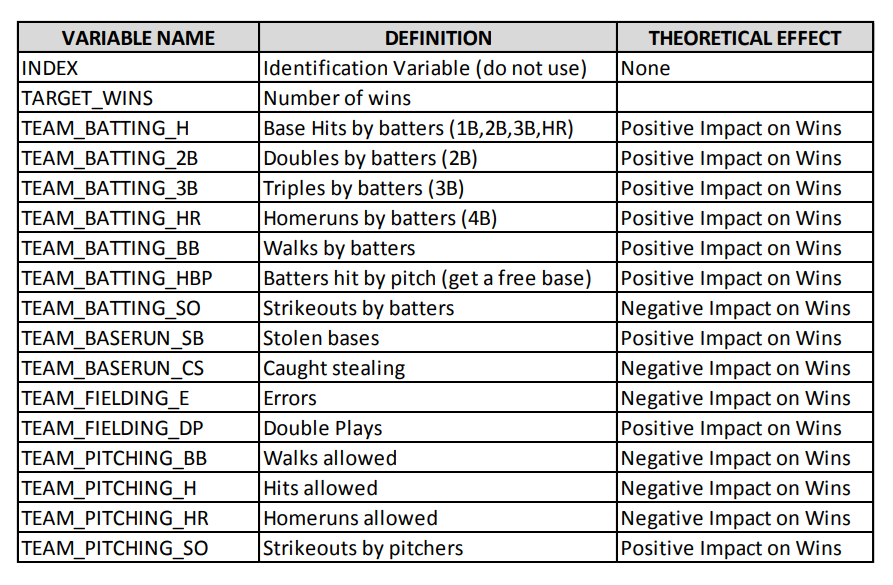
\includegraphics[keepaspectratio]{HW1_DescTable.png}}
\caption{Variable Description Table}
\end{figure}

\subsection{Deliverables:}\label{deliverables}

\begin{itemize}
\tightlist
\item
  A write-up submitted in PDF format. Your write-up should have four
  sections. Each one is described below. You may assume you are
  addressing me as a fellow data scientist, so do not need to shy away
  from technical details.
\item
  Assigned predictions (the number of wins for the team) for the
  evaluation data set.
\item
  Include your R statistical programming code in an Appendix.
\end{itemize}

\subsection{Write Up INSTRUCTIONS:}\label{write-up-instructions}

\paragraph{1) DATA EXPLORATION}\label{data-exploration}

Describe the size and the variables in the moneyball training data set.
Consider that too much detail will cause a manager to lose interest
while too little detail will make the manager consider that you aren't
doing your job. Some suggestions are given below. Please do NOT treat
this as a check list of things to do to complete the assignment. You
should have your own thoughts on what to tell the boss. These are just
ideas. a. Mean / Standard Deviation / Median b. Bar Chart or Box Plot of
the data c.~Is the data correlated to the target variable (or to other
variables?) d.~Are any of the variables missing and need to be imputed
``fixed''?

\paragraph{2) DATA PREPARATION}\label{data-preparation}

Describe how you have transformed the data by changing the original
variables or creating new variables. If you did transform the data or
create new variables, discuss why you did this. Here are some possible
transformations. a. Fix missing values (maybe with a Mean or Median
value) b. Create flags to suggest if a variable was missing c.~Transform
data by putting it into buckets d.~Mathematical transforms such as log
or square root (or use Box-Cox) e. Combine variables (such as ratios or
adding or multiplying) to create new variables

\paragraph{3) BUILD MODELS}\label{build-models}

Using the training data set, build at least three different multiple
linear regression models, using different variables (or the same
variables with different transformations). Since we have not yet covered
automated variable selection methods, you should select the variables
manually (unless you previously learned Forward or Stepwise selection,
etc.). Since you manually selected a variable for inclusion into the
model or exclusion into the model, indicate why this was done. Discuss
the coefficients in the models, do they make sense? For example, if a
team hits a lot of Home Runs, it would be reasonably expected that such
a team would win more games. However, if the coefficient is negative
(suggesting that the team would lose more games), then that needs to be
discussed. Are you keeping the model even though it is counter
intuitive? Why? The boss needs to know.

\paragraph{4) SELECT MODELS}\label{select-models}

Decide on the criteria for selecting the best multiple linear regression
model. Will you select a model with slightly worse performance if it
makes more sense or is more parsimonious? Discuss why you selected your
model. For the multiple linear regression model, will you use a metric
such as Adjusted R2, RMSE, etc.? Be sure to explain how you can make
inferences from the model, discuss multi-collinearity issues (if any),
and discuss other relevant model output. Using the training data set,
evaluate the multiple linear regression model based on: * (a) mean
squared error * (b) R2 * (c) F-statistic * (d) residual plots

Make predictions using the evaluation data set.

\section{---- WRITE UP START ----}\label{write-up-start--}

\subsection{DATA EXPLORATION:}\label{data-exploration-1}

The training data set received had 2276 rows of data, with no duplicate
rows. There were many variables within the initial training data set,
some of which were redundant or aggregate versions of other variables.
After inspection the dependent variable that we want to inspect, and
subsequently predict is TARGET\_WINS. WIth the exception of the INDEX
column, the rest are the independent X variables. Below is a break down
of all of the non-index columns and their respective Null value counts,
along with the range of their values. Note: All of the columns were
continuous integers.

\paragraph{Overview of Non-Index
Columns}\label{overview-of-non-index-columns}

\begin{longtable}[]{@{}
  >{\raggedright\arraybackslash}p{(\linewidth - 8\tabcolsep) * \real{0.3651}}
  >{\raggedright\arraybackslash}p{(\linewidth - 8\tabcolsep) * \real{0.1587}}
  >{\raggedright\arraybackslash}p{(\linewidth - 8\tabcolsep) * \real{0.1270}}
  >{\raggedright\arraybackslash}p{(\linewidth - 8\tabcolsep) * \real{0.2381}}
  >{\raggedright\arraybackslash}p{(\linewidth - 8\tabcolsep) * \real{0.1111}}@{}}
\toprule\noalign{}
\begin{minipage}[b]{\linewidth}\raggedright
Column Name
\end{minipage} & \begin{minipage}[b]{\linewidth}\raggedright
Data Type
\end{minipage} & \begin{minipage}[b]{\linewidth}\raggedright
Nulls
\end{minipage} & \begin{minipage}[b]{\linewidth}\raggedright
Range
\end{minipage} & \begin{minipage}[b]{\linewidth}\raggedright
Notes
\end{minipage} \\
\midrule\noalign{}
\endhead
\bottomrule\noalign{}
\endlastfoot
TARGET\_WINS & \texttt{\textless{}int\textgreater{}} & No Nulls & 0 -
146 & DEPENDENT\_VAR \\
TEAM\_BATTING\_H & \texttt{\textless{}int\textgreater{}} & No Nulls &
891 - 2,554 & \\
TEAM\_BATTING\_2B & \texttt{\textless{}int\textgreater{}} & No Nulls &
69 - 458 & \\
TEAM\_BATTING\_3B & \texttt{\textless{}int\textgreater{}} & No Nulls & 0
- 223 & \\
TEAM\_BATTING\_HR & \texttt{\textless{}int\textgreater{}} & No Nulls & 0
- 264 & \\
TEAM\_BATTING\_BB & \texttt{\textless{}int\textgreater{}} & No Nulls & 0
- 878 & \\
TEAM\_BATTING\_SO & \texttt{\textless{}int\textgreater{}} & 102 Nulls &
0 - 1,399 & \\
TEAM\_BASERUN\_SB & \texttt{\textless{}int\textgreater{}} & 131 Nulls &
0 - 697 & \\
TEAM\_BASERUN\_CS & \texttt{\textless{}int\textgreater{}} & 772 Nulls &
0 - 201 & \\
TEAM\_BATTING\_HBP & \texttt{\textless{}int\textgreater{}} & 2085 Nulls
& 29 - 95 & \\
TEAM\_PITCHING\_H & \texttt{\textless{}int\textgreater{}} & No Nulls &
1,137 - 30,132 & \\
TEAM\_PITCHING\_HR & \texttt{\textless{}int\textgreater{}} & No Nulls &
0 - 343 & \\
TEAM\_PITCHING\_BB & \texttt{\textless{}int\textgreater{}} & No Nulls &
0 - 3,645 & \\
TEAM\_PITCHING\_SO & \texttt{\textless{}int\textgreater{}} & 102 Nulls &
0 - 19,278 & \\
TEAM\_FIELDING\_E & \texttt{\textless{}int\textgreater{}} & No Nulls &
65 - 1,898 & \\
TEAM\_FIELDING\_DP & \texttt{\textless{}int\textgreater{}} & 286 Nulls &
52 - 228 & \\
\end{longtable}

Of these columns there are several that have null values in need of
resolution. After confirming that null values were not just ``zeros in
disguise'', the scale of the presence of nulls in the data was examined,
only 8 percent of rows from the original 2,276 rows have no nulls.
Leading us to conclude strategies for accommodating these null columns
will be necessary. Ultimately, several different techniques were
leveraged. In addition to these techniques there were one or two other
column that were parsed out of larger ``aggregate'' type columns.
Lastly, for a brief overview on all of the initial variable columns and
their relationship to one another for those rows without nulls please
see the chart below:

\emph{GGPairs Table For Training Data}

\begin{figure}
\centering
\pandocbounded{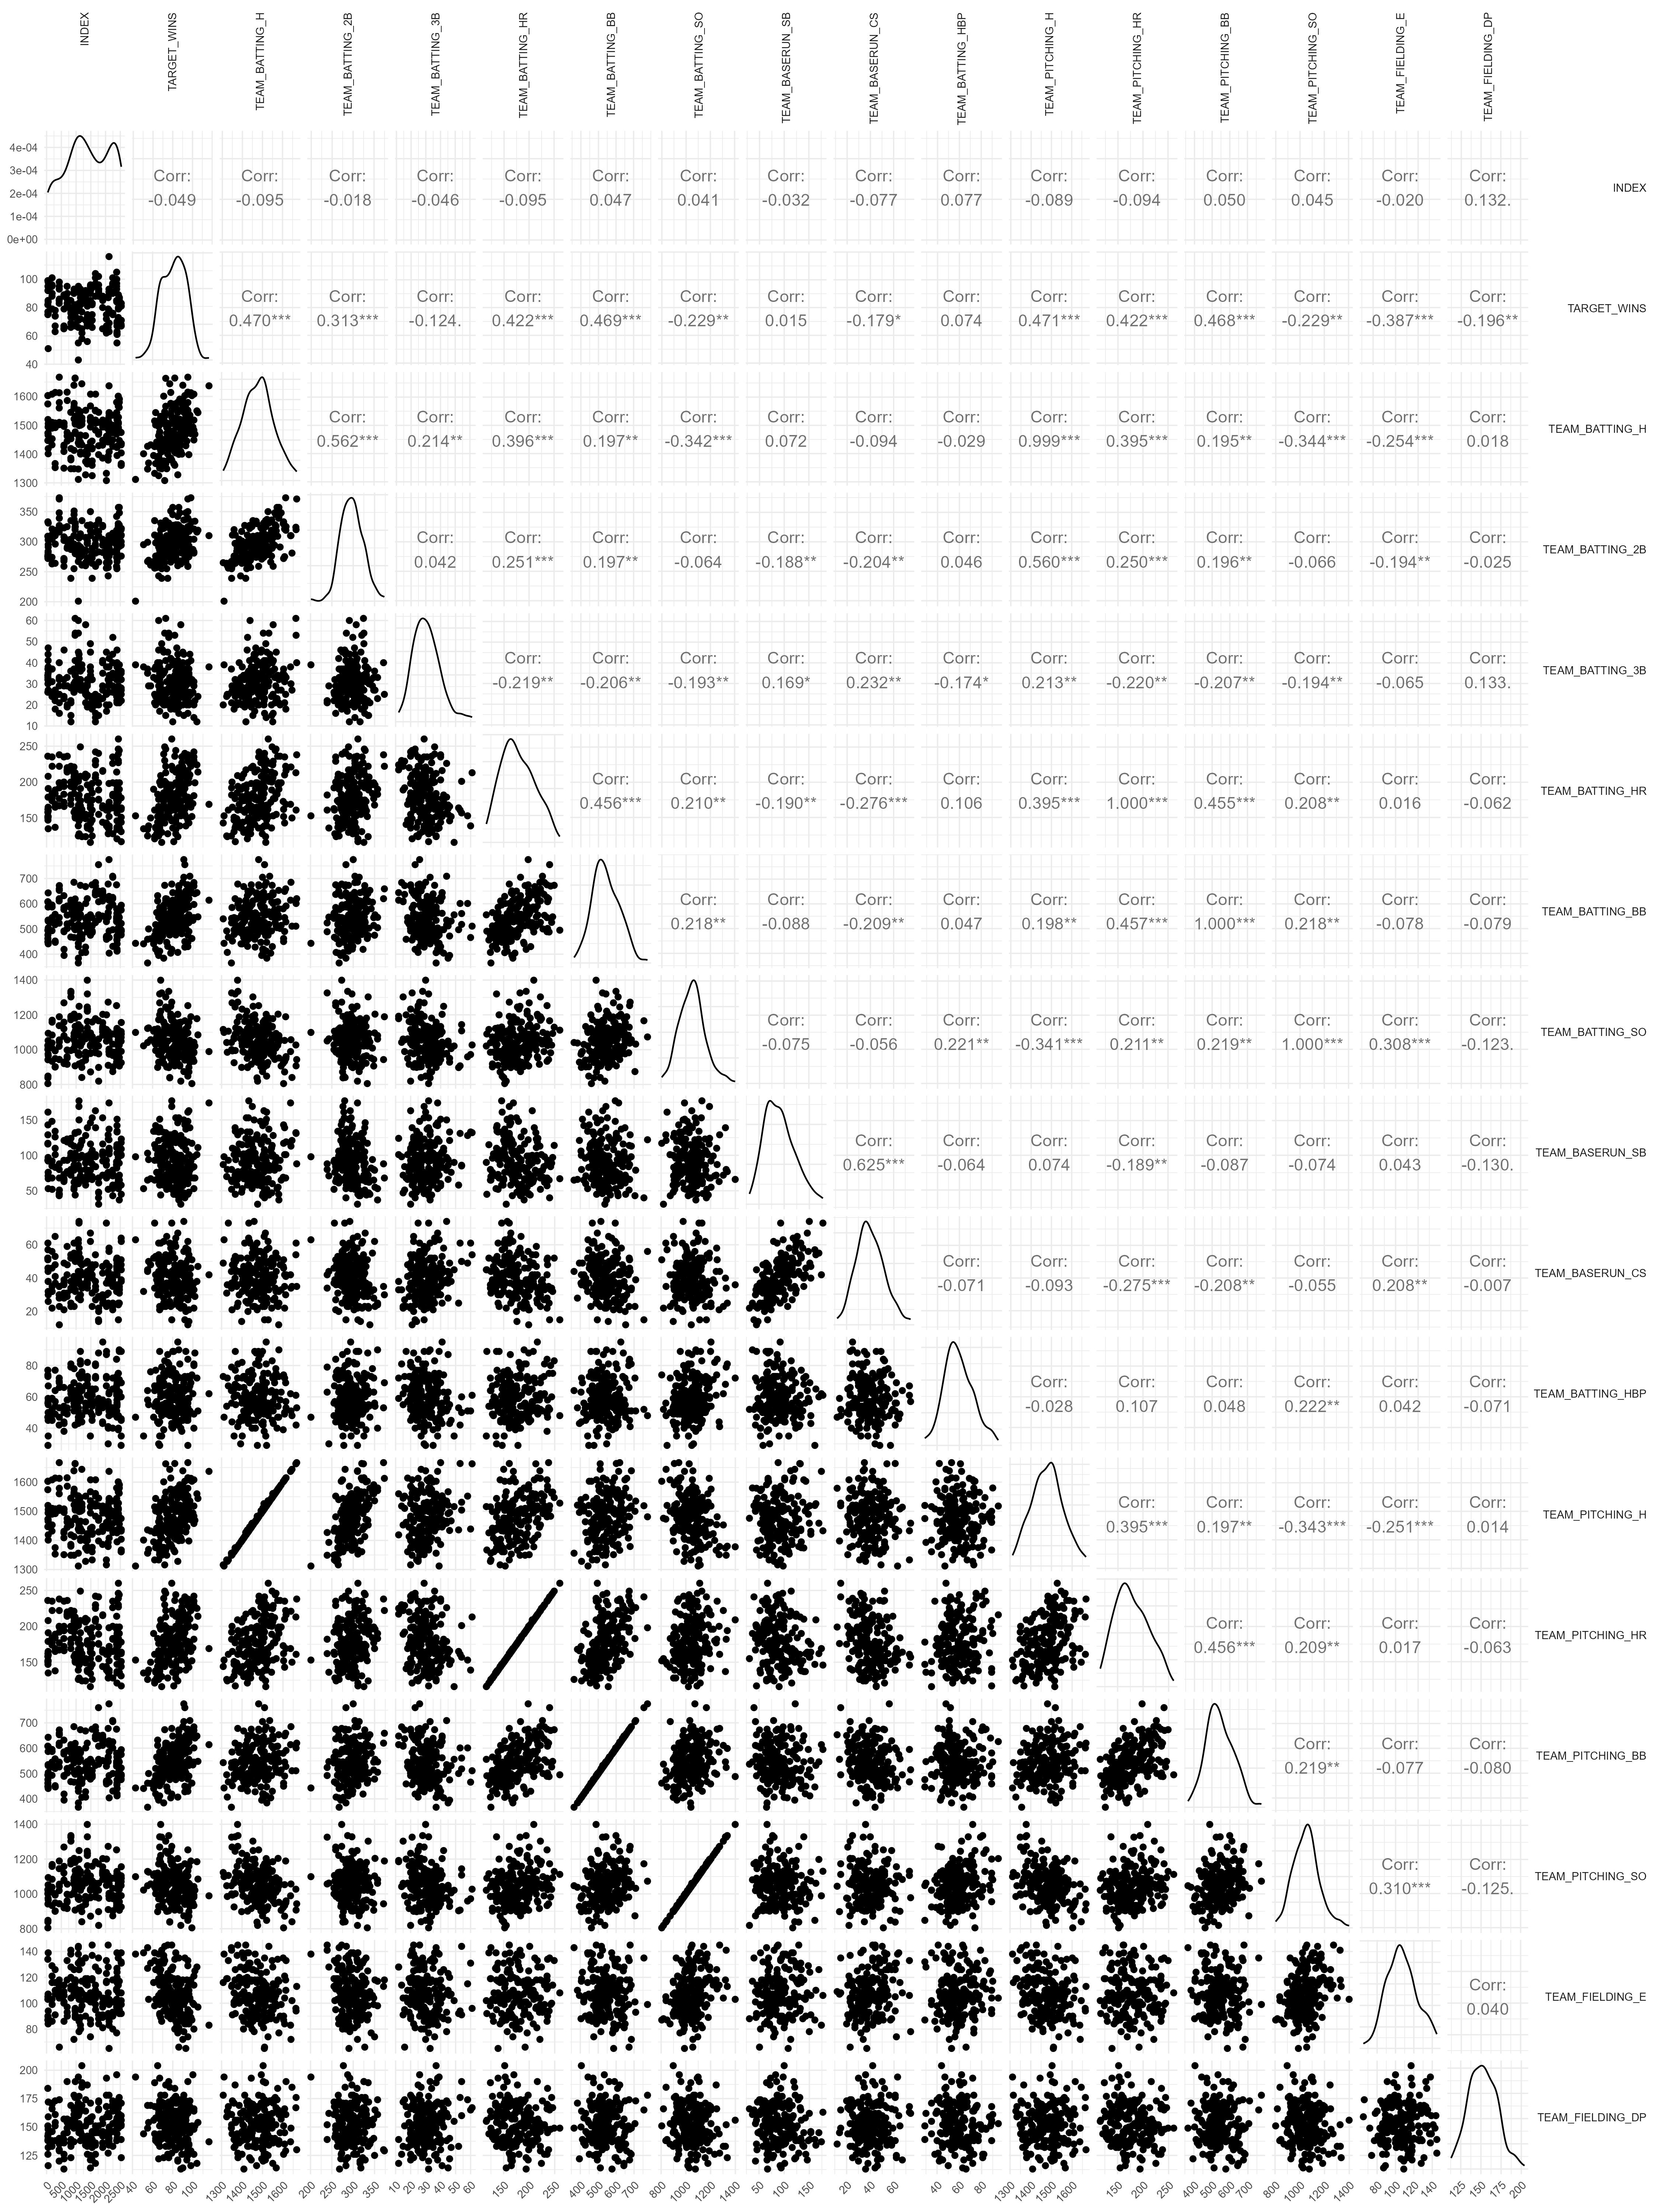
\includegraphics[keepaspectratio]{ggpairs_plot.png}}
\caption{GGPairs Table For Training Data}
\end{figure}

The main takeaways from this glimpse of the raw data with nulls removed
were:

\begin{itemize}
\item
  Several Variables have noticeable Positive relationships and noticable
  negative relationships with the TARGET\_WINS Variable.
\item
  TEAM\_BATTING\_H and TEAM\_PITCHING\_H have a direct linear
  relationship, not independent
\item
  TEAM\_BATTING\_SO and TEAM\_PITCHING\_SO have a direct linear
  relationship, not independent.
\item
  TEAM\_BATTING\_BB and TEAM\_PITCHING\_BB have a direct linear
  relationship, not independent.
\item
  Positive relationship between TEAM\_BASERUN\_SB and TEAM\_BASERUN\_CS,
  may want to merge these to one var.
\end{itemize}

After this initial evaluation, the data cleaning and processing was
carried out.

\subsection{DATA PROCESSING}\label{data-processing}

There were multiple steps taken to process the training data and prepare
it for modeling. Firstly, as mentioned, the columns that contained null
values needed to be addressed. Please see the image below for a coverage
map for the presence of nulls in the training data. Each column with
nulls was examined and addressed with a specific solution. These
solutions were as follows:

\begin{itemize}
\tightlist
\item
  Before imputation several flagging columns were generated in order to
  keep track of which row values were imputed if needed.
\item
  There were enough non-null values for TEAM\_BATTING\_SO and
  TEAM\_PITCHING\_SO, so imputation using the MICE packed with
  Predictive Mean Modeling (PMM) methodology was used. Enough data to
  impute TEAM\_BATTING\_SO and TEAM\_PITCHING\_SO. Need to impute.
\item
  Additionally, before imputation of the TEAM\_PITCHING\_SO column there
  were two rows that contained extreme outliers. These two rows were
  removed from the data before imputation for any data.
\item
  Similarly, the TEAM\_FIELDING\_DP column has 286 Nulls, which was
  roughly 14\% null values. The remaining 1,990 values were used to
  impute values for this nulls using the same MICE PMM methodology.
\item
  The other columns were handled without the use of imputation. This as
  in part due to the large number of null values in the data compared
  with the non null values for select columns. The actions taken were:

  \begin{itemize}
  \tightlist
  \item
    The columns TEAM\_BASERUN\_SB and TEAM\_BASERUN\_CS were combined
    into TEAM\_BASERUN\_STEAL\_ATTEMPTS. This yeilded no nulls for this
    new aggregate column.
  \item
    The columns TEAM\_BATTING\_HBP was combined with TEAM\_BATTING\_BB
    (no null values) to generate TEAM\_BATTING\_WALK\_TOTAL. This
    yielded no null values.
  \end{itemize}
\end{itemize}

\emph{Null Values Visualized with MICE Package}

\begin{figure}
\centering
\pandocbounded{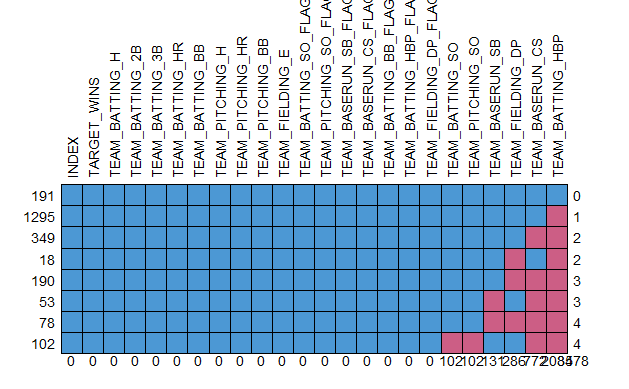
\includegraphics[keepaspectratio]{nullpatterns.png}}
\caption{Null Values Visualized with MICE Package}
\end{figure}

Beyond imputation and accommodating nulls there were other aspects of
the data that were edited, this varied by model and the concept behind
them. These tactics, because they were specific for the models are
discussed in the next section.

\subsection{MODEL BUILDING}\label{model-building}

There were multiple modeling concepts conceived and tested before
ulimately landing on one to use for TARGET\_WINS prediction. The models
that were devised, and their respcective data alterations are as
follows:

\paragraph{1. TARGET\_WINS VS VARIOUS TYPES OF BASE HITS (1, 2, 3, and
HOME
RUNS)}\label{target_wins-vs-various-types-of-base-hits-1-2-3-and-home-runs}

This model sought to examine the types of batting gains with respect to
base number in order to see if there was any significance in variance
explaination for TARGET\_WINS of a team. It parsed out TEAM\_BATTING\_1B
from the larger aggregate TEAM\_BATTING\_H, and modeled the relevant
columns.

\textbf{CUSTOM DATA PROCESSING}

\begin{itemize}
\tightlist
\item
  Parsed out TEAM\_BATTING\_1B from TEAM\_BATTING\_H. This was done by
  subtracting the sum of TEAM\_BATTING\_1B, TEAM\_BATTING\_2B,
  TEAM\_BATTING\_3B, TEAM\_BATTING\_HR from TEAM\_BATTING\_H.
\item
  The TEAM\_BATTING\_H was dropped from the model because of its
  aggregate nature.
\end{itemize}

\textbf{INITIAL MODEL PERFORMANCE}

\emph{MODEL 1 SUMMARY}

\begin{figure}
\centering
\pandocbounded{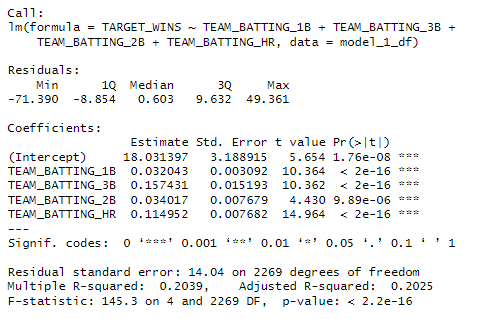
\includegraphics[keepaspectratio]{./model_summary/MODEL1_MAIN.png}}
\caption{MODEL 1 SUMMARY}
\end{figure}

\paragraph{2. TARGET\_WINS VS DEFENSIVE AND OFFENSIVE INDICES (MODEL
ULTIMATELY
SELECTED)}\label{target_wins-vs-defensive-and-offensive-indices-model-ultimately-selected}

This model sought to examine the influences of defense and offensive
actions on the chances of winning the game. These indices were used see
if there was any significance in variance explanation for TARGET\_WINS
of a team. This model was subsequently selected to fine tune and improve
because it was the best performing model.

\textbf{CUSTOM DATA PROCESSING}

\begin{itemize}
\tightlist
\item
  DEFENSE\_INDEX was created by adding up the sum of TEAM\_PITCHING\_SO
  + TEAM\_FIELDING\_DP for a row and subtracting the TEAM\_FIELDING\_E
  column.
\item
  OFFENSE\_INDEX was created by adding up TEAM\_BATTING\_H +
  TEAM\_BATTING\_BB + TEAM\_BASERUN\_SB for a row.
\end{itemize}

\textbf{INITIAL MODEL PERFORMANCE}

\emph{MODEL 2 SUMMARY}

\begin{figure}
\centering
\pandocbounded{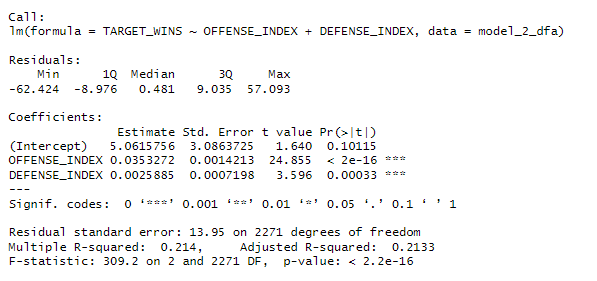
\includegraphics[keepaspectratio]{./model_summary/MODEL2_MAIN.png}}
\caption{MODEL 2 SUMMARY}
\end{figure}

\textbf{SUBMODELS WITH NUANCE}

Within this model, the columns that fed each index were also used in two
separate models in order to get a sense of how each influenced the
model.

\emph{MODEL 2 DEFENSIVE COLUMNS GRANULAR SUMMARY}\\
\pandocbounded{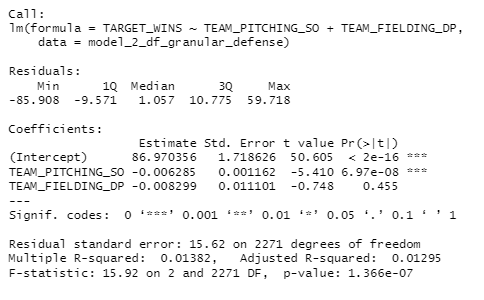
\includegraphics[keepaspectratio]{./model_summary/MODEL2_MAIN_DEFENSIVE_GRANULAR.png}}

\emph{MODEL 2 OFFENSIVE COLUMNS GRANULAR SUMMARY}\\
\pandocbounded{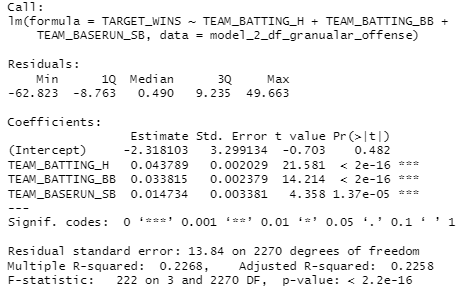
\includegraphics[keepaspectratio]{./model_summary/MODEL2_MAIN_OFFENSIVE_GRANULAR.png}}

\paragraph{3. TARGET\_WINS VS HIGH RISK AND LOW RISK ACTION
INDICES}\label{target_wins-vs-high-risk-and-low-risk-action-indices}

This model sought to examine the influences of high risk and low risk
actions on the chances of winning the game. High risk actions were
multiple base hits, excluding home runs, while low risk behavior
included single base gain hits, walking base gains, and batting home
runs.

\textbf{CUSTOM DATA PROCESSING}

\begin{itemize}
\tightlist
\item
  HIGH RISK INDEX was created by taking the sum of ``high risk'' types
  of playing activity. It summed up TEAM\_BASERUN\_STEAL\_ATTEMPTS,
  TEAM\_BATTING\_2B and TEAM\_BATTING\_3B.
\item
  LOW RISK INDEX was created by taking the sum of ``low risk'' types of
  playing activities. It summed up TEAM\_BATTING\_1B,
  TEAM\_BATTING\_WALK\_TOTAL, and TEAM\_BATTING\_HR.
\end{itemize}

\textbf{INITIAL MODEL PERFORMANCE}

\emph{MODEL 3 SUMMARY}\\
\pandocbounded{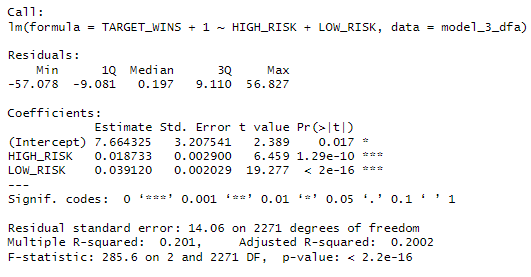
\includegraphics[keepaspectratio]{./model_summary/MODEL3_MAIN.png}}

\textbf{SUBMODELS WITH NUANCE}

Within this model, the columns that fed each index were also used in two
separate models in order to get a sense of how each influenced the
model.

\emph{MODEL 3 HIGH RISK GRANULAR SUMMARY}\\
\pandocbounded{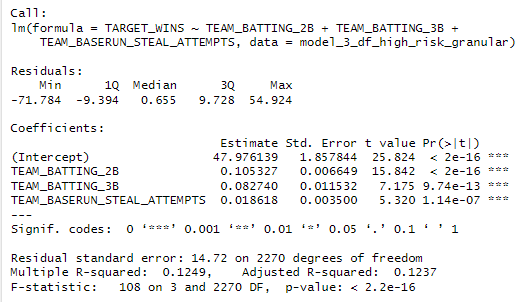
\includegraphics[keepaspectratio]{./model_summary/MODEL3_HIGHRISK_GRANULAR.png}}\\
\emph{MODEL 3 LOW RISK GRANULAR SUMMARY}\\
\pandocbounded{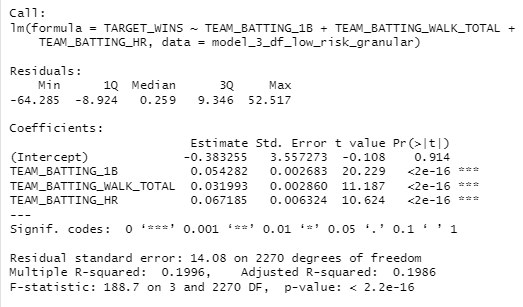
\includegraphics[keepaspectratio]{./model_summary/MODEL3_LOWRISK_GRANULAR.png}}

\paragraph{4. TARGET\_WINS VS DEFENSIVE PITCHING VS DEFENSIVE FIELD
ACTION
INDICES}\label{target_wins-vs-defensive-pitching-vs-defensive-field-action-indices}

This model sought to look at the differences in defensive type actions
on the TARGET\_WINS. Defensive Field activities such as double plays and
errors made when a team is in the field. Defensive Pitch activities took
a look at the Pitcher's strike outs, as well as the pitcher's walks and
hits allowed.

\textbf{CUSTOM DATA PROCESSING}

\begin{itemize}
\tightlist
\item
  FIELD WORK INDEX was created by taking the TEAM\_FIELDING\_DP and
  subtracting the TEAM\_FIELDING\_E column.
\item
  PITCH WORK INDEX was created by taking the TEAM\_PITCHING\_SO and
  subtracting the sum of TEAM\_PITCHING\_BB and TEAM\_PITCHING\_H
  columns.
\end{itemize}

\textbf{INITIAL MODEL PERFORMANCE}

\emph{MODEL 4 SUMMARY}\\
\pandocbounded{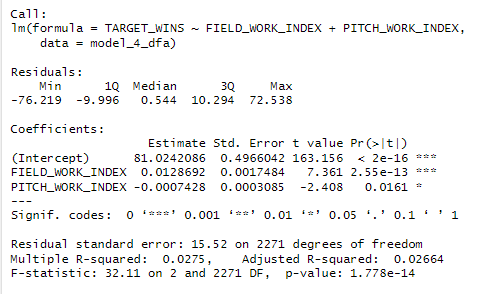
\includegraphics[keepaspectratio]{./model_summary/MODEL4_MAIN.png}}

\textbf{SUBMODELS WITH NUANCE}\\
Within this model, the columns that fed each index were also used in two
separate models in order to get a sense of how each influenced the
model.

\emph{MODEL 4 PITCH WORK GRANULAR SUMMARY}\\
\pandocbounded{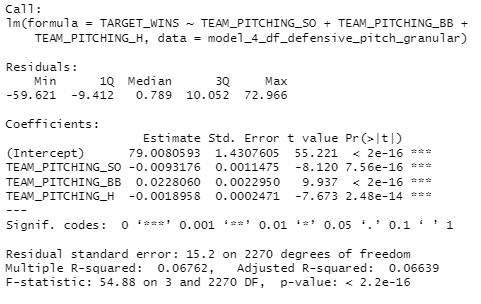
\includegraphics[keepaspectratio]{./model_summary/MODEL4_PITCH_GRANULAR.png}}\\
\emph{MODEL 4 FIELD WORK GRANULAR SUMMARY}\\
\pandocbounded{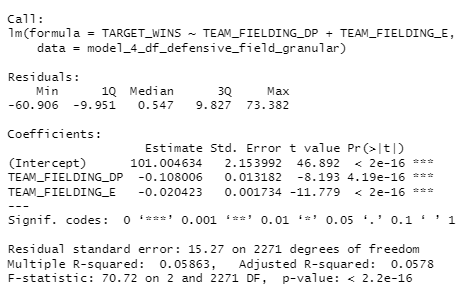
\includegraphics[keepaspectratio]{./model_summary/MODEL4_FIELD_GRANULAR.png}}

\subsection{MODEL SELECTION AND FURTHER
MODIFICATION}\label{model-selection-and-further-modification}

Of all the models that were initially thought of and executed Model 2
was the best performing, so it was ultimately chosen for refinement and
improvement.

\subsubsection{Alterations and Improvements to MODEL
2}\label{alterations-and-improvements-to-model-2}

After selecting MODEL 2 due to its relatively better performance, the
negative valued in the Defense index needed to be corrected before
attempting to use Box-Cox to identify a proper lambda value to help fit
the dependent variable. This was done by shifting the Defense index to
be calulated by dividing the sum of TEAM\_PITCHING\_SO and
TEAM\_FIELDING\_DP by the TEAM\_FIELDING\_E column. This yeilded
positive values for this index. Additionally, for both the Defensive and
Offensive indicies multiple transformations were applied with the
results of each examined in order to determine the best transformation.
These results can be seen in the table below. Lastly, because there were
zeros in the TARGET\_WINS column, this column was altered to have 1
added to it.

\paragraph{TRANSFORMATION COMPARISONS}\label{transformation-comparisons}

\begin{longtable}[]{@{}lll@{}}
\toprule\noalign{}
Transformation & R² (\%) & F-score \\
\midrule\noalign{}
\endhead
\bottomrule\noalign{}
\endlastfoot
No Change (X Vars) & 21.7 & 317 \\
Log Transform & \textbf{22.75} & \textbf{335} \\
Square Root (SqRt) & 22.43 & 329 \\
Squared & 21.17 & 317 \\
Cubed & 21.77 & 317 \\
\end{longtable}

These transformations were applied to the data, and Model 2 was run
again with updated results. You can see below that the transformed model
has normally distributed residuals on the histgram, and mostly normal QQ
plot as well. However, there is some slight deviation at the ends on the
QQ line plot.

\emph{TRANSFORMED MODEL 2 MODEL SUMMARY}\\
\pandocbounded{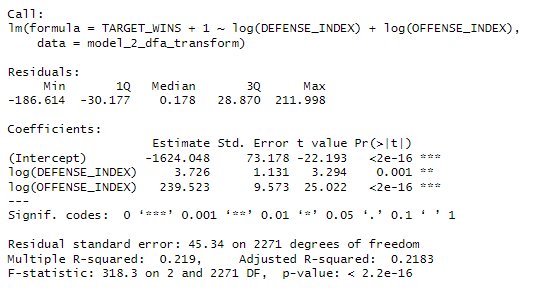
\includegraphics[keepaspectratio]{./model_summary/MODEL2_MAIN_INDEX_FIX.png}}\\
\emph{TRANSFORMED MODEL 2 HISTOGRAM PLOT}\\
\pandocbounded{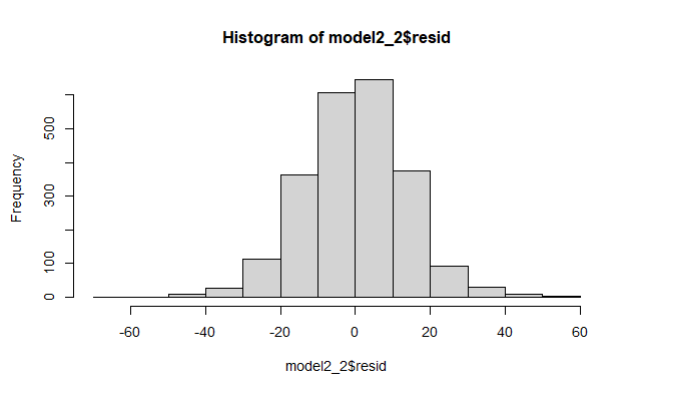
\includegraphics[keepaspectratio]{./model_summary/MODEL2_TRANSFORMED_HIST_RESID.png}}\\
\emph{TRANSFORMED MODEL 2 QQ PLOT}\\
\pandocbounded{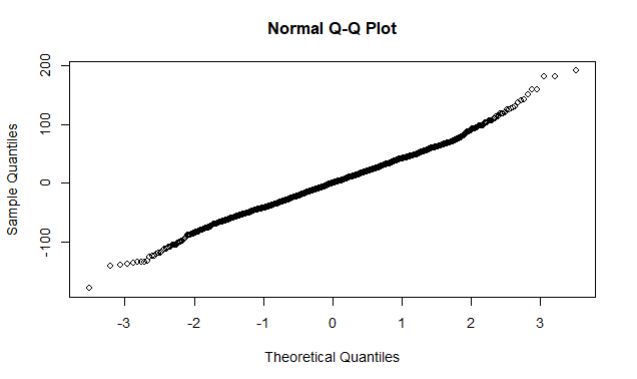
\includegraphics[keepaspectratio]{./model_summary/MODEL2_TRANSFORMED_QQ_RESID.png}}\\
Following these transformations, Box-Cox was used on the best performing
transformed model acquire a lambda value for TARGET\_WINS. The optimal
lambda value was \textasciitilde1.27. The lambda value was applied to
the TARGET\_WINS column, and the model was run.

\emph{TRANSFORMED MODEL 2 BOXCOX MODEL SUMMARY}\\
\pandocbounded{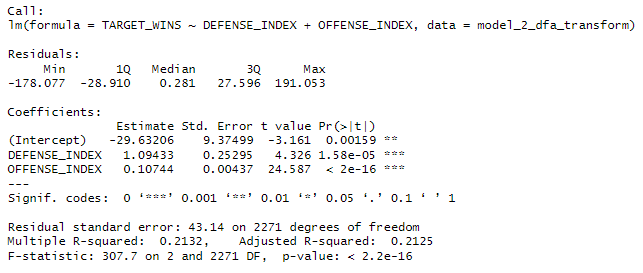
\includegraphics[keepaspectratio]{./model_summary/MODEL2_BCX_IMPROVED.png}}\\
\emph{TRANSFORMED MODEL 2 BOXCOX HISTOGRAM PLOT}\\
\pandocbounded{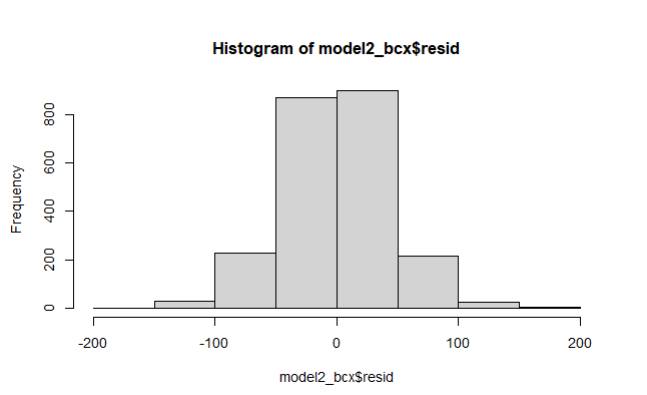
\includegraphics[keepaspectratio]{./model_summary/MODEL2_BCX_HIST_RESID.png}}\\
\emph{TRANSFORMED MODEL 2 BOXCOX QQ PLOT}\\
\pandocbounded{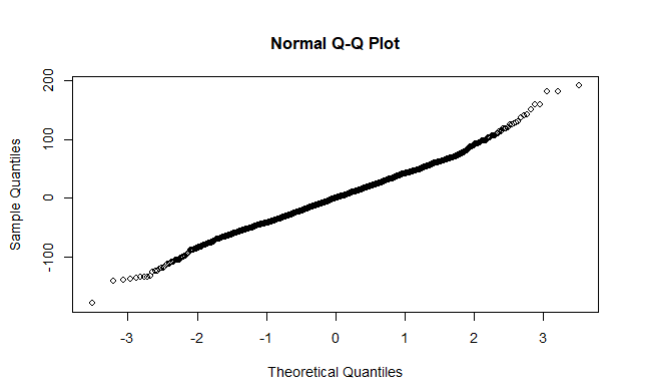
\includegraphics[keepaspectratio]{./model_summary/MODEL2_BCX_QQ_RESID.png}}\\
Overall, the Box Cox lambda application seems to have worsened the model
based on the R\^{}2 and F-Score values, as well as the skewness of it's
residuals, going from a -0.012 with the transformed model to a 0.106
with the Box-Cox lambda application. The MODEL 2 Transformed with logs
and the adjusted Defensive index was the best model of those tried. With
that being said this model still only explained around 21.8 percent of
the variance in the TARGET\_WINS column. The F-Score was fairly high,
helping to support the legitimacy of this modal. The coefficients in
this model indicate that the Offensive Index is more important for the
TARGET\_WIN prediction than the Deffensive index, as their respective
coefficients are 239,5 and 3.72. If there was another variable similar
to TEAM\_FIELD\_E for the offensive side of things to divide by in the
Offensive index i wonder how this would shift the model.

Finally, This model was then used to predict TARGET\_WIN values in the
moneyball\_eval\_data, specifically after the identical restructuring
and processing was completed on that dataset. See below (commented out
for knitting):

\begin{Shaded}
\begin{Highlighting}[]
\CommentTok{\#predictions \textless{}{-} predict(model2\_2, newdata=moneyball\_eval\_formatted)  \# Predict on TestData}

\DocumentationTok{\#\# PREDICTED WINS}
\CommentTok{\#predicted\_win\_data \textless{}{-} cbind(moneyball\_eval\_formatted, PRED\_TARGET\_WINS = predictions)}
\CommentTok{\#head(predicted\_win\_data)}
\end{Highlighting}
\end{Shaded}

The appendix below contains all of my code, most of it relavant to my
thought process and some of it unused scrap.

\subsection{Appendix: R Code}\label{appendix-r-code}

\begin{Shaded}
\begin{Highlighting}[]
\CommentTok{\#Reading in both data sets, However only inspecting the Training Data for now because that is what we want to work with. }

\NormalTok{moneyball\_train\_data }\OtherTok{=} \FunctionTok{read.csv}\NormalTok{(}\FunctionTok{url}\NormalTok{(}\StringTok{"https://raw.githubusercontent.com/jhnboyy/CUNY\_SPS\_WORK/refs/heads/main/Spring2025/DATA621/data/moneyball{-}training{-}data.csv"}\NormalTok{))}
\NormalTok{moneyball\_eval\_data }\OtherTok{=} \FunctionTok{read.csv}\NormalTok{(}\FunctionTok{url}\NormalTok{(}\StringTok{"https://raw.githubusercontent.com/jhnboyy/CUNY\_SPS\_WORK/refs/heads/main/Spring2025/DATA621/data/moneyball{-}evaluation{-}data.csv"}\NormalTok{))}
\end{Highlighting}
\end{Shaded}

\begin{Shaded}
\begin{Highlighting}[]
\CommentTok{\# Taking a look at the first five rows, along with the columns and their respective data types. }
\FunctionTok{print}\NormalTok{(}\FunctionTok{head}\NormalTok{(moneyball\_train\_data))}
\end{Highlighting}
\end{Shaded}

\begin{verbatim}
##   INDEX TARGET_WINS TEAM_BATTING_H TEAM_BATTING_2B TEAM_BATTING_3B
## 1     1          39           1445             194              39
## 2     2          70           1339             219              22
## 3     3          86           1377             232              35
## 4     4          70           1387             209              38
## 5     5          82           1297             186              27
## 6     6          75           1279             200              36
##   TEAM_BATTING_HR TEAM_BATTING_BB TEAM_BATTING_SO TEAM_BASERUN_SB
## 1              13             143             842              NA
## 2             190             685            1075              37
## 3             137             602             917              46
## 4              96             451             922              43
## 5             102             472             920              49
## 6              92             443             973             107
##   TEAM_BASERUN_CS TEAM_BATTING_HBP TEAM_PITCHING_H TEAM_PITCHING_HR
## 1              NA               NA            9364               84
## 2              28               NA            1347              191
## 3              27               NA            1377              137
## 4              30               NA            1396               97
## 5              39               NA            1297              102
## 6              59               NA            1279               92
##   TEAM_PITCHING_BB TEAM_PITCHING_SO TEAM_FIELDING_E TEAM_FIELDING_DP
## 1              927             5456            1011               NA
## 2              689             1082             193              155
## 3              602              917             175              153
## 4              454              928             164              156
## 5              472              920             138              168
## 6              443              973             123              149
\end{verbatim}

\begin{Shaded}
\begin{Highlighting}[]
\DocumentationTok{\#\# Confirming distinct values in df before count and summary }
\FunctionTok{print}\NormalTok{(}\FunctionTok{nrow}\NormalTok{(moneyball\_train\_data)) }\CommentTok{\# 2276}
\end{Highlighting}
\end{Shaded}

\begin{verbatim}
## [1] 2276
\end{verbatim}

\begin{Shaded}
\begin{Highlighting}[]
\NormalTok{moneyball\_train\_data }\OtherTok{\textless{}{-}}\NormalTok{ moneyball\_train\_data }\SpecialCharTok{|\textgreater{}} \FunctionTok{distinct}\NormalTok{()}

\FunctionTok{print}\NormalTok{(}\FunctionTok{nrow}\NormalTok{(moneyball\_train\_data)) }\CommentTok{\# no Dupes, 2276}
\end{Highlighting}
\end{Shaded}

\begin{verbatim}
## [1] 2276
\end{verbatim}

\begin{Shaded}
\begin{Highlighting}[]
\DocumentationTok{\#\#\# Summary Stats of the training data. }
\FunctionTok{print}\NormalTok{(}\FunctionTok{summary}\NormalTok{(moneyball\_train\_data))}
\end{Highlighting}
\end{Shaded}

\begin{verbatim}
##      INDEX         TARGET_WINS     TEAM_BATTING_H TEAM_BATTING_2B
##  Min.   :   1.0   Min.   :  0.00   Min.   : 891   Min.   : 69.0  
##  1st Qu.: 630.8   1st Qu.: 71.00   1st Qu.:1383   1st Qu.:208.0  
##  Median :1270.5   Median : 82.00   Median :1454   Median :238.0  
##  Mean   :1268.5   Mean   : 80.79   Mean   :1469   Mean   :241.2  
##  3rd Qu.:1915.5   3rd Qu.: 92.00   3rd Qu.:1537   3rd Qu.:273.0  
##  Max.   :2535.0   Max.   :146.00   Max.   :2554   Max.   :458.0  
##                                                                  
##  TEAM_BATTING_3B  TEAM_BATTING_HR  TEAM_BATTING_BB TEAM_BATTING_SO 
##  Min.   :  0.00   Min.   :  0.00   Min.   :  0.0   Min.   :   0.0  
##  1st Qu.: 34.00   1st Qu.: 42.00   1st Qu.:451.0   1st Qu.: 548.0  
##  Median : 47.00   Median :102.00   Median :512.0   Median : 750.0  
##  Mean   : 55.25   Mean   : 99.61   Mean   :501.6   Mean   : 735.6  
##  3rd Qu.: 72.00   3rd Qu.:147.00   3rd Qu.:580.0   3rd Qu.: 930.0  
##  Max.   :223.00   Max.   :264.00   Max.   :878.0   Max.   :1399.0  
##                                                    NA's   :102     
##  TEAM_BASERUN_SB TEAM_BASERUN_CS TEAM_BATTING_HBP TEAM_PITCHING_H
##  Min.   :  0.0   Min.   :  0.0   Min.   :29.00    Min.   : 1137  
##  1st Qu.: 66.0   1st Qu.: 38.0   1st Qu.:50.50    1st Qu.: 1419  
##  Median :101.0   Median : 49.0   Median :58.00    Median : 1518  
##  Mean   :124.8   Mean   : 52.8   Mean   :59.36    Mean   : 1779  
##  3rd Qu.:156.0   3rd Qu.: 62.0   3rd Qu.:67.00    3rd Qu.: 1682  
##  Max.   :697.0   Max.   :201.0   Max.   :95.00    Max.   :30132  
##  NA's   :131     NA's   :772     NA's   :2085                    
##  TEAM_PITCHING_HR TEAM_PITCHING_BB TEAM_PITCHING_SO  TEAM_FIELDING_E 
##  Min.   :  0.0    Min.   :   0.0   Min.   :    0.0   Min.   :  65.0  
##  1st Qu.: 50.0    1st Qu.: 476.0   1st Qu.:  615.0   1st Qu.: 127.0  
##  Median :107.0    Median : 536.5   Median :  813.5   Median : 159.0  
##  Mean   :105.7    Mean   : 553.0   Mean   :  817.7   Mean   : 246.5  
##  3rd Qu.:150.0    3rd Qu.: 611.0   3rd Qu.:  968.0   3rd Qu.: 249.2  
##  Max.   :343.0    Max.   :3645.0   Max.   :19278.0   Max.   :1898.0  
##                                    NA's   :102                       
##  TEAM_FIELDING_DP
##  Min.   : 52.0   
##  1st Qu.:131.0   
##  Median :149.0   
##  Mean   :146.4   
##  3rd Qu.:164.0   
##  Max.   :228.0   
##  NA's   :286
\end{verbatim}

\begin{Shaded}
\begin{Highlighting}[]
\DocumentationTok{\#\# Overview Non{-}Index Columns \textless{}datatypes\textgreater{}:  Notes}
\CommentTok{\#TARGET\_WINS \textless{}int\textgreater{}: No nulls, Range: 0 {-} 146}
\CommentTok{\#TEAM\_BATTING\_H \textless{}int\textgreater{}: No Nulls, 891 {-} 2,554}
\CommentTok{\#TEAM\_BATTING\_2B \textless{}int\textgreater{}: No Nulls, 69 {-} 458}
\CommentTok{\#TEAM\_BATTING\_3B \textless{}int\textgreater{}: No Nulls, 0 {-} 223}
\CommentTok{\#TEAM\_BATTING\_HR \textless{}int\textgreater{}: No Nulls, 0 {-} 264}
\CommentTok{\#TEAM\_BATTING\_BB \textless{}int\textgreater{}: No Nulls, 0 {-} 878}
\CommentTok{\#TEAM\_BATTING\_SO \textless{}int\textgreater{}: 102 Nulls, 0 {-} 1,399}
\CommentTok{\#TEAM\_BASERUN\_SB \textless{}int\textgreater{}: 131 Nulls, 0 {-} 697}
\CommentTok{\#TEAM\_BASERUN\_CS \textless{}int\textgreater{}: 772 Nulls, 0 {-} 201}
\CommentTok{\#TEAM\_BATTING\_HBP \textless{}int\textgreater{}: 2085 Nulls, 29 {-} 95}
\CommentTok{\#TEAM\_PITCHING\_H \textless{}int\textgreater{}: No Nulls, 1137 {-} 30,132}
\CommentTok{\#TEAM\_PITCHING\_HR \textless{}int\textgreater{}: No Nulls, 0 {-} 343}
\CommentTok{\#TEAM\_PITCHING\_BB \textless{}int\textgreater{}: No Nulls, 0 {-} 3645}
\CommentTok{\#TEAM\_PITCHING\_SO \textless{}int\textgreater{}: 102 Nulls, 0 {-} 19278}
\CommentTok{\#TEAM\_FIELDING\_E \textless{}int\textgreater{}: No Nulls, 65 {-} 1898}
\CommentTok{\#TEAM\_FIELDING\_DP \textless{}int\textgreater{}: 286 Nulls, 52 {-} 228}

\DocumentationTok{\#\# TARGET\_WINS is the dependent var. }
\DocumentationTok{\#\# The other various predictors would be independent vars. }
\DocumentationTok{\#\# May need to use imputation for some of these because of nulls. }


\DocumentationTok{\#\# Based on Description Table the following relationships may be true: }
\DocumentationTok{\#\# TEAM\_BATTING\_H may be somewhat an aggregate of  TEAM\_BATTING\_2B, TEAM\_BATTING\_3B, TEAM\_BATTING\_HR}
\DocumentationTok{\#\# {-} The sum of the latter three variables minus the TEAM\_BATTING\_H should be "TEAM\_BATTING\_1B"}
\DocumentationTok{\#\# {-} Confirming my Understanding of this: }

\NormalTok{temp\_hit\_df }\OtherTok{\textless{}{-}}\NormalTok{ moneyball\_train\_data  }\SpecialCharTok{|\textgreater{}}
\NormalTok{  dplyr}\SpecialCharTok{::}\FunctionTok{select}\NormalTok{(TEAM\_BATTING\_H,TEAM\_BATTING\_2B, TEAM\_BATTING\_3B, TEAM\_BATTING\_HR) }\SpecialCharTok{|\textgreater{}}
  \FunctionTok{mutate}\NormalTok{(}\StringTok{"TEAM\_BATTING\_1B"} \OtherTok{=}\NormalTok{ TEAM\_BATTING\_H }\SpecialCharTok{{-}}\NormalTok{ (TEAM\_BATTING\_2B}\SpecialCharTok{+}\NormalTok{TEAM\_BATTING\_3B}\SpecialCharTok{+}\NormalTok{TEAM\_BATTING\_HR))}

\FunctionTok{print}\NormalTok{(}\FunctionTok{head}\NormalTok{(temp\_hit\_df))}
\end{Highlighting}
\end{Shaded}

\begin{verbatim}
##   TEAM_BATTING_H TEAM_BATTING_2B TEAM_BATTING_3B TEAM_BATTING_HR
## 1           1445             194              39              13
## 2           1339             219              22             190
## 3           1377             232              35             137
## 4           1387             209              38              96
## 5           1297             186              27             102
## 6           1279             200              36              92
##   TEAM_BATTING_1B
## 1            1199
## 2             908
## 3             973
## 4            1044
## 5             982
## 6             951
\end{verbatim}

\begin{Shaded}
\begin{Highlighting}[]
\DocumentationTok{\#\# Are Errors (TEAM\_FIELDING\_E) and aggregate of the "allowed" categories: TEAM\_PITCHING\_BB,TEAM\_PITCHING\_H,TEAM\_PITCHING\_HR }

\NormalTok{temp\_error\_df }\OtherTok{\textless{}{-}}\NormalTok{ moneyball\_train\_data }\SpecialCharTok{|\textgreater{}}
\NormalTok{  dplyr}\SpecialCharTok{::}\FunctionTok{select}\NormalTok{(TEAM\_FIELDING\_E,TEAM\_PITCHING\_BB,TEAM\_PITCHING\_H,TEAM\_PITCHING\_HR) }\SpecialCharTok{|\textgreater{}}
  \FunctionTok{mutate}\NormalTok{(}\StringTok{"Allowed\_Sum"} \OtherTok{=}\NormalTok{  TEAM\_PITCHING\_BB}\SpecialCharTok{+}\NormalTok{TEAM\_PITCHING\_H}\SpecialCharTok{+}\NormalTok{TEAM\_PITCHING\_HR,}
         \StringTok{"equiv\_test"} \OtherTok{=}\NormalTok{ TEAM\_FIELDING\_E }\SpecialCharTok{==}\NormalTok{ Allowed\_Sum)}

\FunctionTok{print}\NormalTok{(}\FunctionTok{head}\NormalTok{(temp\_error\_df))}
\end{Highlighting}
\end{Shaded}

\begin{verbatim}
##   TEAM_FIELDING_E TEAM_PITCHING_BB TEAM_PITCHING_H TEAM_PITCHING_HR Allowed_Sum
## 1            1011              927            9364               84       10375
## 2             193              689            1347              191        2227
## 3             175              602            1377              137        2116
## 4             164              454            1396               97        1947
## 5             138              472            1297              102        1871
## 6             123              443            1279               92        1814
##   equiv_test
## 1      FALSE
## 2      FALSE
## 3      FALSE
## 4      FALSE
## 5      FALSE
## 6      FALSE
\end{verbatim}

\begin{Shaded}
\begin{Highlighting}[]
\DocumentationTok{\#\# This is not the case, there are no instances where this is true.       }
\NormalTok{temp\_error\_df }\SpecialCharTok{|\textgreater{}} 
  \FunctionTok{filter}\NormalTok{(equiv\_test}\SpecialCharTok{==}\ConstantTok{TRUE}\NormalTok{)}
\end{Highlighting}
\end{Shaded}

\begin{verbatim}
## [1] TEAM_FIELDING_E  TEAM_PITCHING_BB TEAM_PITCHING_H  TEAM_PITCHING_HR
## [5] Allowed_Sum      equiv_test      
## <0 rows> (or 0-length row.names)
\end{verbatim}

\begin{Shaded}
\begin{Highlighting}[]
\DocumentationTok{\#\# According to the descriptive document for this homework, these stats are seasonal perforance for a teams over time (1871 {-} 2006)}
\DocumentationTok{\#\# Curious how many teams are in this data, although there is no way to parse them out. }
\NormalTok{total\_years }\OtherTok{\textless{}{-}} \DecValTok{2006{-}1871}
\FunctionTok{print}\NormalTok{(total\_years)}
\end{Highlighting}
\end{Shaded}

\begin{verbatim}
## [1] 135
\end{verbatim}

\begin{Shaded}
\begin{Highlighting}[]
\CommentTok{\# Combining both aspects of the data because this is the same data but split for this task: }
\NormalTok{total\_rows }\OtherTok{\textless{}{-}} \FunctionTok{nrow}\NormalTok{(moneyball\_train\_data)}\SpecialCharTok{+}\FunctionTok{nrow}\NormalTok{(moneyball\_eval\_data)}

\DocumentationTok{\#\# Total teams covered: }
\FunctionTok{print}\NormalTok{(total\_rows}\SpecialCharTok{/}\NormalTok{total\_years) }\DocumentationTok{\#\# About 18 {-} 19 teams. }
\end{Highlighting}
\end{Shaded}

\begin{verbatim}
## [1] 18.77778
\end{verbatim}

\begin{Shaded}
\begin{Highlighting}[]
\DocumentationTok{\#\# ABOVE TEAM WORK NOT APPLICABLE AFTER REREADING THE DESCROPTION OF THE DATA }
\end{Highlighting}
\end{Shaded}

\begin{Shaded}
\begin{Highlighting}[]
\CommentTok{\# Looking at nulls, For those columns with Nulls See what the other columns look like. Are they the same rows? Are they different rows?}
 
\DocumentationTok{\#\# {-}{-}{-} TEAM\_BATTING\_SO (Batting Strike out nulls)}
\NormalTok{so\_nulls }\OtherTok{\textless{}{-}}\NormalTok{ moneyball\_train\_data }\SpecialCharTok{|\textgreater{}} \FunctionTok{filter}\NormalTok{(}\FunctionTok{is.na}\NormalTok{(TEAM\_BATTING\_SO))}

\CommentTok{\#so\_nulls}

\DocumentationTok{\#\# Seems that TEAM\_BASERUN\_CS,TEAM\_BATTING\_HBP, and TEAM\_PITCHING\_SO are null in the same instances as the the strike out nulls. Lets Check,}

\FunctionTok{print}\NormalTok{(}\FunctionTok{unique}\NormalTok{(so\_nulls}\SpecialCharTok{$}\NormalTok{TEAM\_BASERUN\_CS))}
\end{Highlighting}
\end{Shaded}

\begin{verbatim}
## [1] NA
\end{verbatim}

\begin{Shaded}
\begin{Highlighting}[]
\FunctionTok{print}\NormalTok{(}\FunctionTok{unique}\NormalTok{(so\_nulls}\SpecialCharTok{$}\NormalTok{TEAM\_BATTING\_HBP))}
\end{Highlighting}
\end{Shaded}

\begin{verbatim}
## [1] NA
\end{verbatim}

\begin{Shaded}
\begin{Highlighting}[]
\FunctionTok{print}\NormalTok{(}\FunctionTok{unique}\NormalTok{(so\_nulls}\SpecialCharTok{$}\NormalTok{TEAM\_PITCHING\_SO))}
\end{Highlighting}
\end{Shaded}

\begin{verbatim}
## [1] NA
\end{verbatim}

\begin{Shaded}
\begin{Highlighting}[]
\DocumentationTok{\#\# Confirmed all of these values are null when the Pitching Strike outs are null}

\DocumentationTok{\#\# Are the nulls here just zeros? Lets see if zeros exist anywhere in their respective non null values. }
\DocumentationTok{\#\# Using Summary again: }
\FunctionTok{print}\NormalTok{(}\FunctionTok{summary}\NormalTok{(moneyball\_train\_data))}
\end{Highlighting}
\end{Shaded}

\begin{verbatim}
##      INDEX         TARGET_WINS     TEAM_BATTING_H TEAM_BATTING_2B
##  Min.   :   1.0   Min.   :  0.00   Min.   : 891   Min.   : 69.0  
##  1st Qu.: 630.8   1st Qu.: 71.00   1st Qu.:1383   1st Qu.:208.0  
##  Median :1270.5   Median : 82.00   Median :1454   Median :238.0  
##  Mean   :1268.5   Mean   : 80.79   Mean   :1469   Mean   :241.2  
##  3rd Qu.:1915.5   3rd Qu.: 92.00   3rd Qu.:1537   3rd Qu.:273.0  
##  Max.   :2535.0   Max.   :146.00   Max.   :2554   Max.   :458.0  
##                                                                  
##  TEAM_BATTING_3B  TEAM_BATTING_HR  TEAM_BATTING_BB TEAM_BATTING_SO 
##  Min.   :  0.00   Min.   :  0.00   Min.   :  0.0   Min.   :   0.0  
##  1st Qu.: 34.00   1st Qu.: 42.00   1st Qu.:451.0   1st Qu.: 548.0  
##  Median : 47.00   Median :102.00   Median :512.0   Median : 750.0  
##  Mean   : 55.25   Mean   : 99.61   Mean   :501.6   Mean   : 735.6  
##  3rd Qu.: 72.00   3rd Qu.:147.00   3rd Qu.:580.0   3rd Qu.: 930.0  
##  Max.   :223.00   Max.   :264.00   Max.   :878.0   Max.   :1399.0  
##                                                    NA's   :102     
##  TEAM_BASERUN_SB TEAM_BASERUN_CS TEAM_BATTING_HBP TEAM_PITCHING_H
##  Min.   :  0.0   Min.   :  0.0   Min.   :29.00    Min.   : 1137  
##  1st Qu.: 66.0   1st Qu.: 38.0   1st Qu.:50.50    1st Qu.: 1419  
##  Median :101.0   Median : 49.0   Median :58.00    Median : 1518  
##  Mean   :124.8   Mean   : 52.8   Mean   :59.36    Mean   : 1779  
##  3rd Qu.:156.0   3rd Qu.: 62.0   3rd Qu.:67.00    3rd Qu.: 1682  
##  Max.   :697.0   Max.   :201.0   Max.   :95.00    Max.   :30132  
##  NA's   :131     NA's   :772     NA's   :2085                    
##  TEAM_PITCHING_HR TEAM_PITCHING_BB TEAM_PITCHING_SO  TEAM_FIELDING_E 
##  Min.   :  0.0    Min.   :   0.0   Min.   :    0.0   Min.   :  65.0  
##  1st Qu.: 50.0    1st Qu.: 476.0   1st Qu.:  615.0   1st Qu.: 127.0  
##  Median :107.0    Median : 536.5   Median :  813.5   Median : 159.0  
##  Mean   :105.7    Mean   : 553.0   Mean   :  817.7   Mean   : 246.5  
##  3rd Qu.:150.0    3rd Qu.: 611.0   3rd Qu.:  968.0   3rd Qu.: 249.2  
##  Max.   :343.0    Max.   :3645.0   Max.   :19278.0   Max.   :1898.0  
##                                    NA's   :102                       
##  TEAM_FIELDING_DP
##  Min.   : 52.0   
##  1st Qu.:131.0   
##  Median :149.0   
##  Mean   :146.4   
##  3rd Qu.:164.0   
##  Max.   :228.0   
##  NA's   :286
\end{verbatim}

\begin{Shaded}
\begin{Highlighting}[]
\CommentTok{\#TEAM\_BATTING\_SO {-} Zeros present}
\DocumentationTok{\#\#TEAM\_BASERUN\_SB {-} Zeros present}
\CommentTok{\#TEAM\_BASERUN\_CS {-} Zeros present}
\CommentTok{\#TEAM\_BATTING\_HBP {-} No Zeros}
\CommentTok{\#TEAM\_PITCHING\_SO {-} Zeros present }
\CommentTok{\#TEAM\_FIELDING\_DP {-} No zeros present}

\DocumentationTok{\#\# Most of the columns that have nulls also have zeros, so structurally speaking the nulls are most likely not zeros and will need imputation, or we will need to remove the rows.}

\DocumentationTok{\#\# What proportion of the data is null, would it be worth removing? }
\NormalTok{no\_nulls}\OtherTok{\textless{}{-}}\NormalTok{moneyball\_train\_data }\SpecialCharTok{|\textgreater{}} 
  \FunctionTok{filter}\NormalTok{(}\SpecialCharTok{!}\FunctionTok{is.na}\NormalTok{(TEAM\_BATTING\_SO),}
         \SpecialCharTok{!}\FunctionTok{is.na}\NormalTok{(TEAM\_BASERUN\_SB),}
         \SpecialCharTok{!}\FunctionTok{is.na}\NormalTok{(TEAM\_BASERUN\_CS),}
         \SpecialCharTok{!}\FunctionTok{is.na}\NormalTok{(TEAM\_BATTING\_HBP),}
         \SpecialCharTok{!}\FunctionTok{is.na}\NormalTok{(TEAM\_PITCHING\_SO),}
         \SpecialCharTok{!}\FunctionTok{is.na}\NormalTok{(TEAM\_FIELDING\_DP))}


\CommentTok{\#print(paste("Only", round(nrow(no\_nulls)/ nrow(moneyball\_train\_data),2)*100,"percent of rows from the original",nrow(moneyball\_train\_data),"rows have no nulls, we will need to impute."))}
\end{Highlighting}
\end{Shaded}

\begin{Shaded}
\begin{Highlighting}[]
\DocumentationTok{\#\# Taking a look at the data with pair plots }
\CommentTok{\#colnames(moneyball\_train\_data)}
\CommentTok{\#"TARGET\_WINS", "TEAM\_BATTING\_H"   "TEAM\_BATTING\_2B"  "TEAM\_BATTING\_3B"  "TEAM\_BATTING\_HR"  "TEAM\_BATTING\_BB"  "TEAM\_BATTING\_SO" "TEAM\_BASERUN\_SB"  "TEAM\_BASERUN\_CS"  \#"TEAM\_BATTING\_HBP" "TEAM\_PITCHING\_H"  "TEAM\_PITCHING\_HR" "TEAM\_PITCHING\_BB" "TEAM\_PITCHING\_SO" "TEAM\_FIELDING\_E" "TEAM\_FIELDING\_DP"}

\NormalTok{moneyball\_train\_nona }\OtherTok{\textless{}{-}} \FunctionTok{na.omit}\NormalTok{(moneyball\_train\_data)}
\DocumentationTok{\#\# }\AlertTok{NOTE}\DocumentationTok{ THIS IS A VERY SMALL SUBSET BECAUSE OF THE NULLS }
\FunctionTok{print}\NormalTok{(}\FunctionTok{nrow}\NormalTok{(moneyball\_train\_nona)) }\CommentTok{\#191}
\end{Highlighting}
\end{Shaded}

\begin{verbatim}
## [1] 191
\end{verbatim}

\begin{Shaded}
\begin{Highlighting}[]
\NormalTok{p }\OtherTok{\textless{}{-}} \FunctionTok{ggpairs}\NormalTok{(moneyball\_train\_nona,}
           \AttributeTok{progress =} \ConstantTok{FALSE}\NormalTok{) }\SpecialCharTok{+}  
          \FunctionTok{theme\_minimal}\NormalTok{(}\AttributeTok{base\_size=}\DecValTok{9}\NormalTok{) }\SpecialCharTok{+}
  \FunctionTok{theme}\NormalTok{(}\AttributeTok{axis.text.x =} \FunctionTok{element\_text}\NormalTok{(}\AttributeTok{angle =} \DecValTok{45}\NormalTok{, }\AttributeTok{hjust =} \DecValTok{1}\NormalTok{),}
                                      \AttributeTok{strip.text.x =} \FunctionTok{element\_text}\NormalTok{(}\AttributeTok{angle =} \DecValTok{90}\NormalTok{, }\AttributeTok{hjust =} \DecValTok{1}\NormalTok{),}
                                     \AttributeTok{strip.text.y =} \FunctionTok{element\_text}\NormalTok{(}\AttributeTok{angle =} \DecValTok{0}\NormalTok{, }\AttributeTok{hjust =} \DecValTok{1}\NormalTok{))}
\DocumentationTok{\#\# Saving Image for reference in PDF \#}
\CommentTok{\#ggsave("ggpairs\_plot.png", plot = p, width = 15, height = 20, units = "in", dpi = 300)}

\DocumentationTok{\#\#\# Notesworthy Points from the GGPAIRs plot. }
\CommentTok{\#{-}{-} TEAM\_BATTING\_H and TEAM\_PITCHING\_H have a direct linear relationship, not independent}
\CommentTok{\#{-}{-} TEAM\_BATTING\_SO and TEAM\_PITCHING\_SO have a direct linear relationship, not independent.}
\CommentTok{\#{-}{-} TEAM\_BATTING\_BB and TEAM\_PITCHING\_BB have a direct linear relationship, not independent.}
\CommentTok{\#{-}{-} Positive relationship between TEAM\_BASERUN\_SB and TEAM\_BASERUN\_CS, may want to merge these to one var. }
\CommentTok{\#{-}{-} There may be some other relationships that slip past the visual checks, but will deal with those later. }

\DocumentationTok{\#\#\# Action Items for modeling:}
\DocumentationTok{\#\# Should keep just one of each of these variables when modeling for sake of predictor independence.}
\DocumentationTok{\#\# Similarly, we should parse out the 1H from the TEAM\_BATTING\_H or just keep only the agg var for modeling. }
\DocumentationTok{\#\# Similar actions needed for TEAM\_PITCHING\_H and TEAM\_PITCHING\_HR, these variables are related as HR is a subset of hits.}
\DocumentationTok{\#\# TEAM\_BASERUN\_SB and TEAM\_BASERUN\_CS aggregated into one Stealing base index, because noticable relationship in plot}
\end{Highlighting}
\end{Shaded}

\begin{Shaded}
\begin{Highlighting}[]
\DocumentationTok{\#\# Looking at the columns with nulls. }

\DocumentationTok{\#\# Plot work for moneyball\_train\_data$TEAM\_BATTING\_SO }
\FunctionTok{ggplot}\NormalTok{(moneyball\_train\_data, }\FunctionTok{aes}\NormalTok{(}\AttributeTok{x =}\NormalTok{ TEAM\_BATTING\_SO)) }\SpecialCharTok{+}
  \FunctionTok{geom\_histogram}\NormalTok{( }\AttributeTok{bins =} \DecValTok{50}\NormalTok{) }\SpecialCharTok{+}
  \FunctionTok{labs}\NormalTok{(}\AttributeTok{title =} \StringTok{"Histogram for TEAM\_BATTING\_SO"}\NormalTok{) }\SpecialCharTok{+}
  \FunctionTok{theme\_minimal}\NormalTok{()}
\end{Highlighting}
\end{Shaded}

\begin{verbatim}
## Warning: Removed 102 rows containing non-finite outside the scale range
## (`stat_bin()`).
\end{verbatim}

\pandocbounded{\includegraphics[keepaspectratio]{DATA621_Homework1_files/figure-latex/ImputationEvaluation1-1.pdf}}

\begin{Shaded}
\begin{Highlighting}[]
\FunctionTok{ggplot}\NormalTok{(moneyball\_train\_data, }\FunctionTok{aes}\NormalTok{(}\AttributeTok{sample =}\NormalTok{ TEAM\_BATTING\_SO)) }\SpecialCharTok{+}
  \FunctionTok{stat\_qq}\NormalTok{() }\SpecialCharTok{+}
  \FunctionTok{theme\_minimal}\NormalTok{()}
\end{Highlighting}
\end{Shaded}

\begin{verbatim}
## Warning: Removed 102 rows containing non-finite outside the scale range
## (`stat_qq()`).
\end{verbatim}

\pandocbounded{\includegraphics[keepaspectratio]{DATA621_Homework1_files/figure-latex/ImputationEvaluation1-2.pdf}}

\begin{Shaded}
\begin{Highlighting}[]
\DocumentationTok{\#\# Distribution conclusion: Not normal, camel shaped }

\DocumentationTok{\#\# Plot work for moneyball\_train\_data$TEAM\_BASERUN\_CS }
\FunctionTok{ggplot}\NormalTok{(moneyball\_train\_data, }\FunctionTok{aes}\NormalTok{(}\AttributeTok{x =}\NormalTok{ TEAM\_BASERUN\_CS)) }\SpecialCharTok{+}
  \FunctionTok{geom\_histogram}\NormalTok{( }\AttributeTok{bins =} \DecValTok{50}\NormalTok{) }\SpecialCharTok{+}
  \FunctionTok{labs}\NormalTok{(}\AttributeTok{title =} \StringTok{"Histogram for TEAM\_BASERUN\_CS"}\NormalTok{) }\SpecialCharTok{+}
  \FunctionTok{theme\_minimal}\NormalTok{()}
\end{Highlighting}
\end{Shaded}

\begin{verbatim}
## Warning: Removed 772 rows containing non-finite outside the scale range
## (`stat_bin()`).
\end{verbatim}

\pandocbounded{\includegraphics[keepaspectratio]{DATA621_Homework1_files/figure-latex/ImputationEvaluation1-3.pdf}}

\begin{Shaded}
\begin{Highlighting}[]
\FunctionTok{ggplot}\NormalTok{(moneyball\_train\_data, }\FunctionTok{aes}\NormalTok{(}\AttributeTok{sample =}\NormalTok{ TEAM\_BASERUN\_CS)) }\SpecialCharTok{+}
  \FunctionTok{stat\_qq}\NormalTok{() }\SpecialCharTok{+}
  \FunctionTok{theme\_minimal}\NormalTok{()}
\end{Highlighting}
\end{Shaded}

\begin{verbatim}
## Warning: Removed 772 rows containing non-finite outside the scale range
## (`stat_qq()`).
\end{verbatim}

\pandocbounded{\includegraphics[keepaspectratio]{DATA621_Homework1_files/figure-latex/ImputationEvaluation1-4.pdf}}

\begin{Shaded}
\begin{Highlighting}[]
\DocumentationTok{\#\# Distribution conclusion: Right Skew in the data, not normal}

\DocumentationTok{\#\# Plot work for moneyball\_train\_data$TEAM\_BASERUN\_SB}
\FunctionTok{ggplot}\NormalTok{(moneyball\_train\_data, }\FunctionTok{aes}\NormalTok{(}\AttributeTok{x =}\NormalTok{ TEAM\_BASERUN\_SB)) }\SpecialCharTok{+}
  \FunctionTok{geom\_histogram}\NormalTok{( }\AttributeTok{bins =} \DecValTok{50}\NormalTok{) }\SpecialCharTok{+}
  \FunctionTok{labs}\NormalTok{(}\AttributeTok{title =} \StringTok{"Histogram for TEAM\_BASERUN\_SB"}\NormalTok{) }\SpecialCharTok{+}
  \FunctionTok{theme\_minimal}\NormalTok{()}
\end{Highlighting}
\end{Shaded}

\begin{verbatim}
## Warning: Removed 131 rows containing non-finite outside the scale range
## (`stat_bin()`).
\end{verbatim}

\pandocbounded{\includegraphics[keepaspectratio]{DATA621_Homework1_files/figure-latex/ImputationEvaluation1-5.pdf}}

\begin{Shaded}
\begin{Highlighting}[]
\FunctionTok{ggplot}\NormalTok{(moneyball\_train\_data, }\FunctionTok{aes}\NormalTok{(}\AttributeTok{sample =}\NormalTok{ TEAM\_BASERUN\_SB)) }\SpecialCharTok{+}
  \FunctionTok{stat\_qq}\NormalTok{() }\SpecialCharTok{+}
  \FunctionTok{theme\_minimal}\NormalTok{()}
\end{Highlighting}
\end{Shaded}

\begin{verbatim}
## Warning: Removed 131 rows containing non-finite outside the scale range
## (`stat_qq()`).
\end{verbatim}

\pandocbounded{\includegraphics[keepaspectratio]{DATA621_Homework1_files/figure-latex/ImputationEvaluation1-6.pdf}}

\begin{Shaded}
\begin{Highlighting}[]
\DocumentationTok{\#\# Distribution conclusion: Right Skew in the data, not normal.}

\DocumentationTok{\#\# Plot work for moneyball\_train\_data$TEAM\_BATTING\_HBP}
\FunctionTok{ggplot}\NormalTok{(moneyball\_train\_data, }\FunctionTok{aes}\NormalTok{(}\AttributeTok{x =}\NormalTok{ TEAM\_BATTING\_HBP)) }\SpecialCharTok{+}
  \FunctionTok{geom\_histogram}\NormalTok{( }\AttributeTok{bins =} \DecValTok{50}\NormalTok{) }\SpecialCharTok{+}
  \FunctionTok{labs}\NormalTok{(}\AttributeTok{title =} \StringTok{"Histogram for TEAM\_BATTING\_HBP"}\NormalTok{) }\SpecialCharTok{+}
  \FunctionTok{theme\_minimal}\NormalTok{()}
\end{Highlighting}
\end{Shaded}

\begin{verbatim}
## Warning: Removed 2085 rows containing non-finite outside the scale range
## (`stat_bin()`).
\end{verbatim}

\pandocbounded{\includegraphics[keepaspectratio]{DATA621_Homework1_files/figure-latex/ImputationEvaluation1-7.pdf}}

\begin{Shaded}
\begin{Highlighting}[]
\FunctionTok{ggplot}\NormalTok{(moneyball\_train\_data, }\FunctionTok{aes}\NormalTok{(}\AttributeTok{sample =}\NormalTok{ TEAM\_BATTING\_HBP)) }\SpecialCharTok{+}
  \FunctionTok{stat\_qq}\NormalTok{() }\SpecialCharTok{+}
  \FunctionTok{theme\_minimal}\NormalTok{()}
\end{Highlighting}
\end{Shaded}

\begin{verbatim}
## Warning: Removed 2085 rows containing non-finite outside the scale range
## (`stat_qq()`).
\end{verbatim}

\pandocbounded{\includegraphics[keepaspectratio]{DATA621_Homework1_files/figure-latex/ImputationEvaluation1-8.pdf}}

\begin{Shaded}
\begin{Highlighting}[]
\DocumentationTok{\#\# Distribution conclusion: Seems normal. Easily seen when bin number is lowered, qq plot mostly comfirms}

\DocumentationTok{\#\# Plot work for moneyball\_train\_data$TEAM\_PITCHING\_SO}
\FunctionTok{ggplot}\NormalTok{(moneyball\_train\_data, }\FunctionTok{aes}\NormalTok{(}\AttributeTok{x =} \DecValTok{1}\SpecialCharTok{+}\FunctionTok{log}\NormalTok{(TEAM\_PITCHING\_SO))) }\SpecialCharTok{+}
  \FunctionTok{geom\_histogram}\NormalTok{( }\AttributeTok{bins =} \DecValTok{50}\NormalTok{) }\SpecialCharTok{+}
  \FunctionTok{labs}\NormalTok{(}\AttributeTok{title =} \StringTok{"Histogram for TEAM\_PITCHING\_SO"}\NormalTok{) }\SpecialCharTok{+}
  \FunctionTok{theme\_minimal}\NormalTok{()}
\end{Highlighting}
\end{Shaded}

\begin{verbatim}
## Warning: Removed 122 rows containing non-finite outside the scale range
## (`stat_bin()`).
\end{verbatim}

\pandocbounded{\includegraphics[keepaspectratio]{DATA621_Homework1_files/figure-latex/ImputationEvaluation1-9.pdf}}

\begin{Shaded}
\begin{Highlighting}[]
\FunctionTok{ggplot}\NormalTok{(moneyball\_train\_data, }\FunctionTok{aes}\NormalTok{(}\AttributeTok{sample =}\NormalTok{ TEAM\_PITCHING\_SO)) }\SpecialCharTok{+}
  \FunctionTok{stat\_qq}\NormalTok{() }\SpecialCharTok{+}
  \FunctionTok{theme\_minimal}\NormalTok{()}
\end{Highlighting}
\end{Shaded}

\begin{verbatim}
## Warning: Removed 102 rows containing non-finite outside the scale range
## (`stat_qq()`).
\end{verbatim}

\pandocbounded{\includegraphics[keepaspectratio]{DATA621_Homework1_files/figure-latex/ImputationEvaluation1-10.pdf}}

\begin{Shaded}
\begin{Highlighting}[]
\DocumentationTok{\#\# Distribution conclusion: Seems normal, with a super high outlier. May need to deal with this}
\FunctionTok{summary}\NormalTok{(moneyball\_train\_data}\SpecialCharTok{$}\NormalTok{TEAM\_PITCHING\_SO) }
\end{Highlighting}
\end{Shaded}

\begin{verbatim}
##    Min. 1st Qu.  Median    Mean 3rd Qu.    Max.    NA's 
##     0.0   615.0   813.5   817.7   968.0 19278.0     102
\end{verbatim}

\begin{Shaded}
\begin{Highlighting}[]
\FunctionTok{sort}\NormalTok{(}\FunctionTok{unique}\NormalTok{(moneyball\_train\_data}\SpecialCharTok{$}\NormalTok{TEAM\_PITCHING\_SO)) }\DocumentationTok{\#\# Two very large outliers: 12758, 19278}
\end{Highlighting}
\end{Shaded}

\begin{verbatim}
##   [1]     0   181   205   208   252   270   272   292   301   306   310   316
##  [13]   320   326   329   341   345   358   361   362   363   364   366   367
##  [25]   369   373   374   375   376   378   380   381   383   384   386   387
##  [37]   390   391   392   393   395   396   398   400   401   402   406   407
##  [49]   409   410   411   412   414   416   417   419   420   422   423   426
##  [61]   427   431   432   433   434   436   437   438   440   443   444   446
##  [73]   447   448   449   450   451   454   455   459   460   461   462   463
##  [85]   464   465   466   467   468   469   470   471   473   475   477   478
##  [97]   479   480   481   483   484   485   486   488   489   490   491   493
## [109]   494   495   496   497   498   499   500   502   503   504   505   506
## [121]   507   508   510   511   512   513   514   515   516   517   518   519
## [133]   520   521   522   524   525   526   527   528   529   530   531   533
## [145]   534   535   536   537   539   540   541   542   543   545   546   547
## [157]   548   549   551   552   553   554   555   556   557   558   559   560
## [169]   561   562   563   564   565   566   567   568   569   570   571   572
## [181]   573   574   575   576   577   578   579   580   581   582   583   584
## [193]   585   586   587   588   589   590   591   592   593   594   595   596
## [205]   597   598   599   600   601   602   603   604   605   606   607   608
## [217]   609   610   611   612   613   614   615   616   617   619   620   621
## [229]   622   623   624   625   626   627   628   629   630   631   633   634
## [241]   635   636   637   638   639   640   641   642   643   644   645   646
## [253]   647   648   649   650   651   652   653   654   655   656   657   658
## [265]   659   660   661   662   663   664   665   666   667   668   669   670
## [277]   671   672   673   674   675   678   679   680   681   682   683   684
## [289]   685   686   687   688   690   691   692   693   694   695   696   697
## [301]   698   700   702   703   704   705   707   708   709   710   711   712
## [313]   713   714   715   716   717   718   719   720   721   722   723   724
## [325]   725   726   727   728   729   730   731   732   733   734   735   736
## [337]   737   738   739   740   741   742   743   744   745   746   747   749
## [349]   750   751   752   753   754   755   756   757   758   759   760   761
## [361]   762   764   765   766   767   768   769   770   771   772   774   775
## [373]   777   778   779   781   782   784   785   787   788   789   790   791
## [385]   792   793   794   795   796   797   799   800   801   802   803   804
## [397]   805   806   807   808   809   810   811   812   813   814   815   816
## [409]   817   818   819   820   821   822   823   824   825   826   827   828
## [421]   829   830   831   832   833   834   835   836   837   838   839   840
## [433]   841   842   843   844   845   846   847   848   849   850   851   852
## [445]   853   854   855   856   857   858   860   861   862   863   864   865
## [457]   866   867   868   869   870   871   872   873   874   875   876   877
## [469]   879   880   881   882   883   884   885   887   888   889   890   891
## [481]   892   893   896   897   898   899   900   901   902   903   904   905
## [493]   906   907   908   909   910   911   912   913   914   915   916   917
## [505]   918   919   920   921   922   923   924   925   926   927   928   929
## [517]   930   931   932   933   934   935   936   937   938   939   940   941
## [529]   942   943   944   946   947   948   949   950   951   952   953   954
## [541]   955   956   957   958   959   960   961   962   963   964   965   966
## [553]   967   968   969   970   971   972   973   974   975   976   977   978
## [565]   979   980   981   982   983   984   985   986   987   988   989   990
## [577]   992   993   994   995   996   997   998  1000  1001  1003  1004  1005
## [589]  1006  1008  1009  1010  1011  1012  1013  1014  1015  1016  1018  1019
## [601]  1020  1021  1022  1023  1024  1025  1026  1027  1028  1029  1030  1031
## [613]  1032  1033  1034  1035  1036  1037  1038  1039  1040  1041  1042  1043
## [625]  1044  1045  1046  1047  1048  1049  1052  1053  1054  1055  1056  1057
## [637]  1058  1059  1060  1061  1062  1063  1066  1067  1068  1069  1070  1071
## [649]  1072  1073  1074  1075  1076  1077  1078  1079  1080  1081  1082  1083
## [661]  1084  1085  1087  1088  1089  1090  1091  1092  1093  1094  1095  1096
## [673]  1097  1098  1099  1102  1103  1104  1105  1106  1107  1108  1109  1110
## [685]  1111  1112  1113  1114  1116  1117  1119  1120  1121  1122  1123  1124
## [697]  1125  1126  1129  1130  1132  1133  1134  1136  1138  1141  1143  1144
## [709]  1145  1146  1148  1153  1155  1156  1157  1158  1159  1160  1161  1162
## [721]  1164  1167  1168  1169  1170  1172  1173  1176  1179  1180  1181  1185
## [733]  1188  1189  1190  1191  1192  1193  1194  1197  1198  1200  1203  1204
## [745]  1205  1206  1208  1210  1211  1217  1221  1222  1233  1237  1239  1245
## [757]  1247  1248  1249  1253  1256  1257  1258  1261  1269  1273  1275  1276
## [769]  1284  1293  1296  1299  1303  1305  1313  1326  1328  1335  1342  1349
## [781]  1350  1351  1354  1356  1364  1370  1371  1385  1386  1387  1399  1405
## [793]  1412  1419  1424  1427  1430  1434  1436  1459  1461  1464  1474  1481
## [805]  1491  1511  1541  1552  1561  1590  1600  1659  1739  1781  2225  2309
## [817]  2367  2492  3450  4224  5456 12758 19278
\end{verbatim}

\begin{Shaded}
\begin{Highlighting}[]
\DocumentationTok{\#\# Is this ONLY two rows? }
\FunctionTok{nrow}\NormalTok{(moneyball\_train\_data }\SpecialCharTok{|\textgreater{}} \FunctionTok{filter}\NormalTok{(TEAM\_PITCHING\_SO}\SpecialCharTok{\textgreater{}}\DecValTok{12000}\NormalTok{)) }\CommentTok{\# Confirmed only two rows, may just want ot remove these. }
\end{Highlighting}
\end{Shaded}

\begin{verbatim}
## [1] 2
\end{verbatim}

\begin{Shaded}
\begin{Highlighting}[]
\NormalTok{moneyball\_train\_data }\SpecialCharTok{|\textgreater{}} \FunctionTok{filter}\NormalTok{(TEAM\_PITCHING\_SO}\SpecialCharTok{\textgreater{}}\DecValTok{12000}\NormalTok{)}
\end{Highlighting}
\end{Shaded}

\begin{verbatim}
##   INDEX TARGET_WINS TEAM_BATTING_H TEAM_BATTING_2B TEAM_BATTING_3B
## 1  1494         108           1188             338               0
## 2  2380          41            992             263              20
##   TEAM_BATTING_HR TEAM_BATTING_BB TEAM_BATTING_SO TEAM_BASERUN_SB
## 1               0             270             945              NA
## 2               0             142             952              NA
##   TEAM_BASERUN_CS TEAM_BATTING_HBP TEAM_PITCHING_H TEAM_PITCHING_HR
## 1              NA               NA           16038                0
## 2              NA               NA           20088                0
##   TEAM_PITCHING_BB TEAM_PITCHING_SO TEAM_FIELDING_E TEAM_FIELDING_DP
## 1             3645            12758             716               NA
## 2             2876            19278             952               NA
\end{verbatim}

\begin{Shaded}
\begin{Highlighting}[]
\DocumentationTok{\#\# Plot work for moneyball\_train\_data$TEAM\_FIELDING\_DP}
\FunctionTok{ggplot}\NormalTok{(moneyball\_train\_data, }\FunctionTok{aes}\NormalTok{(}\AttributeTok{x =}\NormalTok{ TEAM\_FIELDING\_DP)) }\SpecialCharTok{+}
  \FunctionTok{geom\_histogram}\NormalTok{( }\AttributeTok{bins =} \DecValTok{50}\NormalTok{) }\SpecialCharTok{+}
  \FunctionTok{labs}\NormalTok{(}\AttributeTok{title =} \StringTok{"Histogram for TEAM\_FIELDING\_DP"}\NormalTok{) }\SpecialCharTok{+}
  \FunctionTok{theme\_minimal}\NormalTok{()}
\end{Highlighting}
\end{Shaded}

\begin{verbatim}
## Warning: Removed 286 rows containing non-finite outside the scale range
## (`stat_bin()`).
\end{verbatim}

\pandocbounded{\includegraphics[keepaspectratio]{DATA621_Homework1_files/figure-latex/ImputationEvaluation1-11.pdf}}

\begin{Shaded}
\begin{Highlighting}[]
\FunctionTok{ggplot}\NormalTok{(moneyball\_train\_data, }\FunctionTok{aes}\NormalTok{(}\AttributeTok{sample =}\NormalTok{ TEAM\_FIELDING\_DP)) }\SpecialCharTok{+}
  \FunctionTok{stat\_qq}\NormalTok{() }\SpecialCharTok{+}
  \FunctionTok{theme\_minimal}\NormalTok{()}
\end{Highlighting}
\end{Shaded}

\begin{verbatim}
## Warning: Removed 286 rows containing non-finite outside the scale range
## (`stat_qq()`).
\end{verbatim}

\pandocbounded{\includegraphics[keepaspectratio]{DATA621_Homework1_files/figure-latex/ImputationEvaluation1-12.pdf}}

\begin{Shaded}
\begin{Highlighting}[]
\DocumentationTok{\#\# Distribution conclusion: Seems normal}
\end{Highlighting}
\end{Shaded}

\begin{Shaded}
\begin{Highlighting}[]
\CommentTok{\#, fig.width = 5, fig.height =10\}}
\DocumentationTok{\#\# Using Mice Native tool to example the pattern of nulls:}
\DocumentationTok{\#\#Imputation Reference: https://www.r{-}bloggers.com/2015/10/imputing{-}missing{-}data{-}with{-}r{-}mice{-}package/}
\CommentTok{\#md.pattern(moneyball\_train\_data,rotate.names = TRUE)}


\DocumentationTok{\#\# Viz Notes: }
\CommentTok{\#{-} Enough data to impute TEAM\_BATTING\_SO and TEAM\_PITCHING\_SO. Need to impute. }
\CommentTok{\#{-} TEAM\_BASERUN\_CS and TEAM\_BASERUN\_SB it may be worth just to agg to a column that is total attempts at base stealing for team, as this strategy\textquotesingle{}s impact is what we want to know.No need to impute}
\CommentTok{\#{-} Can probably combine the TEAM\_BATTING\_HBP and TEAM\_BATTING\_BB as they are essentially equivalents for impact on game. As total batting walks. No need to impute with HBP because way too many nulls.}

\DocumentationTok{\#\# Looking into TEAM\_FIELDING\_DP (286 Nulls vs)}

\FunctionTok{nrow}\NormalTok{(moneyball\_train\_data }\SpecialCharTok{|\textgreater{}} \FunctionTok{filter}\NormalTok{(}\SpecialCharTok{!}\FunctionTok{is.na}\NormalTok{(TEAM\_FIELDING\_DP)))}\CommentTok{\#1,990 non null rows can impute. \textasciitilde{}14\% nulls}
\end{Highlighting}
\end{Shaded}

\begin{verbatim}
## [1] 1990
\end{verbatim}

\begin{Shaded}
\begin{Highlighting}[]
\DocumentationTok{\#\#\# Takeaways for Imputation Process:}
\CommentTok{\# {-} I was going to try different methods within MICE, but decided to just keep all of them PMM in order to be consistent for explaining. The TEAM\_PITCHING\_SO outliers shouild be handled separately though. }
\CommentTok{\# {-} Overall To Do\textquotesingle{}s: }
\CommentTok{\# {-}{-}{-} TEAM\_BATTING\_SO {-} Imputation with MICE PMM Needed}
\CommentTok{\# {-}{-}{-} TEAM\_PITCHING\_SO {-} Imputation with MICE PMM Needed (Probably need to remove the two outliers from the TEAM\_PITCHING\_SO column before imputation)}
\CommentTok{\# {-}{-}{-} TEAM\_BASERUN\_SB and TEAM\_BASERUN\_CS to be combined into TEAM\_BASERUN\_STEAL\_ATTEMPTS; No Imputation needed.}
\CommentTok{\# {-}{-}{-} TEAM\_BATTING\_HBP can be combined with TEAM\_BATTING\_BB (no null values) into TEAM\_BATTING\_WALK\_TOTAL}
\CommentTok{\# {-}{-}{-} TEAM\_FIELDING\_DP {-}Imputation with MICE PMM Needed}
\end{Highlighting}
\end{Shaded}

\begin{Shaded}
\begin{Highlighting}[]
\DocumentationTok{\#\#\# USING ACTION ITEMS AS GUIDE}
\DocumentationTok{\#\# Adding imputation /missing data Flags to keep track of the changes:}
\DocumentationTok{\#\# Present (P) and Missing (M)}
\NormalTok{moneyball\_train\_data}\SpecialCharTok{$}\NormalTok{TEAM\_BATTING\_SO\_FLAG }\OtherTok{\textless{}{-}} \FunctionTok{ifelse}\NormalTok{(}\FunctionTok{is.na}\NormalTok{(moneyball\_train\_data}\SpecialCharTok{$}\NormalTok{TEAM\_BATTING\_SO), }\StringTok{\textquotesingle{}M\textquotesingle{}}\NormalTok{, }\StringTok{\textquotesingle{}P\textquotesingle{}}\NormalTok{)}
\NormalTok{moneyball\_train\_data}\SpecialCharTok{$}\NormalTok{TEAM\_PITCHING\_SO\_FLAG }\OtherTok{\textless{}{-}} \FunctionTok{ifelse}\NormalTok{(}\FunctionTok{is.na}\NormalTok{(moneyball\_train\_data}\SpecialCharTok{$}\NormalTok{TEAM\_PITCHING\_SO), }\StringTok{\textquotesingle{}M\textquotesingle{}}\NormalTok{, }\StringTok{\textquotesingle{}P\textquotesingle{}}\NormalTok{)}
\NormalTok{moneyball\_train\_data}\SpecialCharTok{$}\NormalTok{TEAM\_BASERUN\_SB\_FLAG }\OtherTok{\textless{}{-}} \FunctionTok{ifelse}\NormalTok{(}\FunctionTok{is.na}\NormalTok{(moneyball\_train\_data}\SpecialCharTok{$}\NormalTok{TEAM\_BASERUN\_SB), }\StringTok{\textquotesingle{}M\textquotesingle{}}\NormalTok{, }\StringTok{\textquotesingle{}P\textquotesingle{}}\NormalTok{)}
\NormalTok{moneyball\_train\_data}\SpecialCharTok{$}\NormalTok{TEAM\_BASERUN\_CS\_FLAG }\OtherTok{\textless{}{-}} \FunctionTok{ifelse}\NormalTok{(}\FunctionTok{is.na}\NormalTok{(moneyball\_train\_data}\SpecialCharTok{$}\NormalTok{TEAM\_BASERUN\_CS), }\StringTok{\textquotesingle{}M\textquotesingle{}}\NormalTok{, }\StringTok{\textquotesingle{}P\textquotesingle{}}\NormalTok{)}
\NormalTok{moneyball\_train\_data}\SpecialCharTok{$}\NormalTok{TEAM\_BATTING\_BB\_FLAG }\OtherTok{\textless{}{-}} \FunctionTok{ifelse}\NormalTok{(}\FunctionTok{is.na}\NormalTok{(moneyball\_train\_data}\SpecialCharTok{$}\NormalTok{TEAM\_BATTING\_BB), }\StringTok{\textquotesingle{}M\textquotesingle{}}\NormalTok{, }\StringTok{\textquotesingle{}P\textquotesingle{}}\NormalTok{)}
\NormalTok{moneyball\_train\_data}\SpecialCharTok{$}\NormalTok{TEAM\_BATTING\_HBP\_FLAG }\OtherTok{\textless{}{-}} \FunctionTok{ifelse}\NormalTok{(}\FunctionTok{is.na}\NormalTok{(moneyball\_train\_data}\SpecialCharTok{$}\NormalTok{TEAM\_BATTING\_HBP), }\StringTok{\textquotesingle{}M\textquotesingle{}}\NormalTok{, }\StringTok{\textquotesingle{}P\textquotesingle{}}\NormalTok{)}
\NormalTok{moneyball\_train\_data}\SpecialCharTok{$}\NormalTok{TEAM\_FIELDING\_DP\_FLAG }\OtherTok{\textless{}{-}} \FunctionTok{ifelse}\NormalTok{(}\FunctionTok{is.na}\NormalTok{(moneyball\_train\_data}\SpecialCharTok{$}\NormalTok{TEAM\_FIELDING\_DP), }\StringTok{\textquotesingle{}M\textquotesingle{}}\NormalTok{, }\StringTok{\textquotesingle{}P\textquotesingle{}}\NormalTok{)}


\CommentTok{\# {-}{-}{-} TEAM\_BASERUN\_SB and TEAM\_BASERUN\_CS to be combined into TEAM\_BASERUN\_STEAL\_ATTEMPTS; No Imputation needed for certain models}
\CommentTok{\# {-}{-}{-} TEAM\_BATTING\_HBP can be combined with TEAM\_BATTING\_BB (no null values) into TEAM\_BATTING\_WALK\_TOTAL}
\NormalTok{moneyball\_train\_processed }\OtherTok{\textless{}{-}}\NormalTok{ moneyball\_train\_data }\SpecialCharTok{|\textgreater{}} 
  \FunctionTok{mutate}\NormalTok{(}\AttributeTok{TEAM\_BASERUN\_STEAL\_ATTEMPTS =} \FunctionTok{ifelse}\NormalTok{(}\FunctionTok{is.na}\NormalTok{(TEAM\_BASERUN\_SB), }\DecValTok{0}\NormalTok{, TEAM\_BASERUN\_SB) }\SpecialCharTok{+} \FunctionTok{ifelse}\NormalTok{(}\FunctionTok{is.na}\NormalTok{(TEAM\_BASERUN\_CS), }\DecValTok{0}\NormalTok{, TEAM\_BASERUN\_CS),}
         \AttributeTok{TEAM\_BATTING\_WALK\_TOTAL =} \FunctionTok{ifelse}\NormalTok{(}\FunctionTok{is.na}\NormalTok{(TEAM\_BATTING\_BB), }\DecValTok{0}\NormalTok{, TEAM\_BATTING\_BB) }\SpecialCharTok{+} \FunctionTok{ifelse}\NormalTok{(}\FunctionTok{is.na}\NormalTok{(TEAM\_BATTING\_HBP), }\DecValTok{0}\NormalTok{, TEAM\_BATTING\_HBP)) }\SpecialCharTok{|\textgreater{}}
\NormalTok{  dplyr}\SpecialCharTok{::}\FunctionTok{select}\NormalTok{(}\SpecialCharTok{{-}}\NormalTok{TEAM\_BASERUN\_CS, }\SpecialCharTok{{-}}\NormalTok{TEAM\_BATTING\_HBP) }\CommentTok{\#{-}TEAM\_BASERUN\_SB,{-}TEAM\_BATTING\_BB}
\DocumentationTok{\#\# In these aggregate derivative rows, im considering the nulls to be zero for summation. }

 

\CommentTok{\# {-}{-}{-} TEAM\_PITCHING\_SO,TEAM\_BATTING\_SO,TEAM\_FIELDING\_DP,TEAM\_BASERUN\_SB,TEAM\_BATTING\_BB {-} Imputation with MICE PMM Needed. Probably need to remove the two outlier columns from the TEAM\_PITCHING\_SO column, and the data at large.}
\NormalTok{outlier\_rows }\OtherTok{\textless{}{-}}\NormalTok{ moneyball\_train\_processed }\SpecialCharTok{|\textgreater{}} \FunctionTok{filter}\NormalTok{(TEAM\_PITCHING\_SO}\SpecialCharTok{\textgreater{}}\DecValTok{12000}\NormalTok{)}
\NormalTok{no\_outlier\_moneyball\_train\_processed }\OtherTok{\textless{}{-}}\NormalTok{ moneyball\_train\_processed }\SpecialCharTok{|\textgreater{}} \FunctionTok{filter}\NormalTok{(TEAM\_PITCHING\_SO}\SpecialCharTok{\textless{}}\DecValTok{12000} \SpecialCharTok{|} \FunctionTok{is.na}\NormalTok{(TEAM\_PITCHING\_SO))}
\NormalTok{imputed }\OtherTok{\textless{}{-}} \FunctionTok{mice}\NormalTok{(no\_outlier\_moneyball\_train\_processed,}\AttributeTok{m=}\DecValTok{5}\NormalTok{,}\AttributeTok{meth=}\StringTok{\textquotesingle{}pmm\textquotesingle{}}\NormalTok{,}\AttributeTok{seed=}\DecValTok{5}\NormalTok{)}
\end{Highlighting}
\end{Shaded}

\begin{verbatim}
## 
##  iter imp variable
##   1   1  TEAM_BATTING_SO  TEAM_BASERUN_SB  TEAM_PITCHING_SO  TEAM_FIELDING_DP
##   1   2  TEAM_BATTING_SO  TEAM_BASERUN_SB  TEAM_PITCHING_SO  TEAM_FIELDING_DP
##   1   3  TEAM_BATTING_SO  TEAM_BASERUN_SB  TEAM_PITCHING_SO  TEAM_FIELDING_DP
##   1   4  TEAM_BATTING_SO  TEAM_BASERUN_SB  TEAM_PITCHING_SO  TEAM_FIELDING_DP
##   1   5  TEAM_BATTING_SO  TEAM_BASERUN_SB  TEAM_PITCHING_SO  TEAM_FIELDING_DP
##   2   1  TEAM_BATTING_SO  TEAM_BASERUN_SB  TEAM_PITCHING_SO  TEAM_FIELDING_DP
##   2   2  TEAM_BATTING_SO  TEAM_BASERUN_SB  TEAM_PITCHING_SO  TEAM_FIELDING_DP
##   2   3  TEAM_BATTING_SO  TEAM_BASERUN_SB  TEAM_PITCHING_SO  TEAM_FIELDING_DP
##   2   4  TEAM_BATTING_SO  TEAM_BASERUN_SB  TEAM_PITCHING_SO  TEAM_FIELDING_DP
##   2   5  TEAM_BATTING_SO  TEAM_BASERUN_SB  TEAM_PITCHING_SO  TEAM_FIELDING_DP
##   3   1  TEAM_BATTING_SO  TEAM_BASERUN_SB  TEAM_PITCHING_SO  TEAM_FIELDING_DP
##   3   2  TEAM_BATTING_SO  TEAM_BASERUN_SB  TEAM_PITCHING_SO  TEAM_FIELDING_DP
##   3   3  TEAM_BATTING_SO  TEAM_BASERUN_SB  TEAM_PITCHING_SO  TEAM_FIELDING_DP
##   3   4  TEAM_BATTING_SO  TEAM_BASERUN_SB  TEAM_PITCHING_SO  TEAM_FIELDING_DP
##   3   5  TEAM_BATTING_SO  TEAM_BASERUN_SB  TEAM_PITCHING_SO  TEAM_FIELDING_DP
##   4   1  TEAM_BATTING_SO  TEAM_BASERUN_SB  TEAM_PITCHING_SO  TEAM_FIELDING_DP
##   4   2  TEAM_BATTING_SO  TEAM_BASERUN_SB  TEAM_PITCHING_SO  TEAM_FIELDING_DP
##   4   3  TEAM_BATTING_SO  TEAM_BASERUN_SB  TEAM_PITCHING_SO  TEAM_FIELDING_DP
##   4   4  TEAM_BATTING_SO  TEAM_BASERUN_SB  TEAM_PITCHING_SO  TEAM_FIELDING_DP
##   4   5  TEAM_BATTING_SO  TEAM_BASERUN_SB  TEAM_PITCHING_SO  TEAM_FIELDING_DP
##   5   1  TEAM_BATTING_SO  TEAM_BASERUN_SB  TEAM_PITCHING_SO  TEAM_FIELDING_DP
##   5   2  TEAM_BATTING_SO  TEAM_BASERUN_SB  TEAM_PITCHING_SO  TEAM_FIELDING_DP
##   5   3  TEAM_BATTING_SO  TEAM_BASERUN_SB  TEAM_PITCHING_SO  TEAM_FIELDING_DP
##   5   4  TEAM_BATTING_SO  TEAM_BASERUN_SB  TEAM_PITCHING_SO  TEAM_FIELDING_DP
##   5   5  TEAM_BATTING_SO  TEAM_BASERUN_SB  TEAM_PITCHING_SO  TEAM_FIELDING_DP
\end{verbatim}

\begin{verbatim}
## Warning: Number of logged events: 7
\end{verbatim}

\begin{Shaded}
\begin{Highlighting}[]
\NormalTok{moneyball\_train\_imputed}\OtherTok{\textless{}{-}}\FunctionTok{complete}\NormalTok{(imputed)}

\CommentTok{\#Checking for nulls where there shouldnt be.}
\FunctionTok{print}\NormalTok{(}\FunctionTok{nrow}\NormalTok{(moneyball\_train\_imputed }\SpecialCharTok{|\textgreater{}} \FunctionTok{filter}\NormalTok{(}\FunctionTok{is.na}\NormalTok{(TEAM\_PITCHING\_SO))))}
\end{Highlighting}
\end{Shaded}

\begin{verbatim}
## [1] 0
\end{verbatim}

\begin{Shaded}
\begin{Highlighting}[]
\DocumentationTok{\#\# Working DF }
\FunctionTok{print}\NormalTok{(}\FunctionTok{head}\NormalTok{(moneyball\_train\_imputed))}
\end{Highlighting}
\end{Shaded}

\begin{verbatim}
##   INDEX TARGET_WINS TEAM_BATTING_H TEAM_BATTING_2B TEAM_BATTING_3B
## 1     1          39           1445             194              39
## 2     2          70           1339             219              22
## 3     3          86           1377             232              35
## 4     4          70           1387             209              38
## 5     5          82           1297             186              27
## 6     6          75           1279             200              36
##   TEAM_BATTING_HR TEAM_BATTING_BB TEAM_BATTING_SO TEAM_BASERUN_SB
## 1              13             143             842              39
## 2             190             685            1075              37
## 3             137             602             917              46
## 4              96             451             922              43
## 5             102             472             920              49
## 6              92             443             973             107
##   TEAM_PITCHING_H TEAM_PITCHING_HR TEAM_PITCHING_BB TEAM_PITCHING_SO
## 1            9364               84              927             5456
## 2            1347              191              689             1082
## 3            1377              137              602              917
## 4            1396               97              454              928
## 5            1297              102              472              920
## 6            1279               92              443              973
##   TEAM_FIELDING_E TEAM_FIELDING_DP TEAM_BATTING_SO_FLAG TEAM_PITCHING_SO_FLAG
## 1            1011              190                    P                     P
## 2             193              155                    P                     P
## 3             175              153                    P                     P
## 4             164              156                    P                     P
## 5             138              168                    P                     P
## 6             123              149                    P                     P
##   TEAM_BASERUN_SB_FLAG TEAM_BASERUN_CS_FLAG TEAM_BATTING_BB_FLAG
## 1                    M                    M                    P
## 2                    P                    P                    P
## 3                    P                    P                    P
## 4                    P                    P                    P
## 5                    P                    P                    P
## 6                    P                    P                    P
##   TEAM_BATTING_HBP_FLAG TEAM_FIELDING_DP_FLAG TEAM_BASERUN_STEAL_ATTEMPTS
## 1                     M                     M                           0
## 2                     M                     P                          65
## 3                     M                     P                          73
## 4                     M                     P                          73
## 5                     M                     P                          88
## 6                     M                     P                         166
##   TEAM_BATTING_WALK_TOTAL
## 1                     143
## 2                     685
## 3                     602
## 4                     451
## 5                     472
## 6                     443
\end{verbatim}

\begin{Shaded}
\begin{Highlighting}[]
\DocumentationTok{\#\# Now that the data is imputed, and some of the columns have been aggregated, taking the next step in processing and/or variable preparation and selection for the models. }
\DocumentationTok{\#\# Printing this to look at the columns again: }
\CommentTok{\#colnames(moneyball\_train\_imputed)}

\DocumentationTok{\#\# Thoughts}
\CommentTok{\#{-} Batting vs BaseRun vs Fielding vs Pitching Agg vars {-}\textgreater{} Offesne vs Defense }
\CommentTok{\#{-} Parse out the 1HB, se can do a correlation with the type of hits vs total wins. }
\CommentTok{\#{-} Steals vs caught steals, maybe also this coirrelation with the hits? }
\CommentTok{\#{-} Need to keep in mind we need to predict winds for the team.}


\DocumentationTok{\#\# Three main Model Ideas that will dictate further processing: }
\CommentTok{\# {-}{-}{-} MODEL 1: Parse out "TEAM\_BATTING\_1B" from TEAM\_BATTING\_H, then can do analysis on the different types of base hits and their correlation with wins. }
\CommentTok{\# {-}{-}{-} MODEL 2: Aggregate into Two index Defense and Offense (Pitching and Field VAS Batting and Baserun Metrics) to see which is more important }
\CommentTok{\# {-}{-}{-} MODEL 3: High Risk Offensive Model, Looking at if the "higher risk" offensive plays are worth it. }
\CommentTok{\# {-}{-}{-} MODEL 4: Pitching Index Model vs Field Index for Defense analysis. }

\DocumentationTok{\#\#\#\# Keeping two dfs for each model (except 1), one with the non aggregated values and one with custom agg vars.}

\DocumentationTok{\#\#\# MODEL 1 Processing }
\CommentTok{\# {-}{-}{-} Limiting to TARGET\_WINS and the parsed out Hit columns}
\NormalTok{model\_1\_df }\OtherTok{\textless{}{-}}\NormalTok{ moneyball\_train\_imputed }\SpecialCharTok{|\textgreater{}} 
\NormalTok{  dplyr}\SpecialCharTok{::}\FunctionTok{select}\NormalTok{(TARGET\_WINS,TEAM\_BATTING\_H,TEAM\_BATTING\_2B,TEAM\_BATTING\_3B,TEAM\_BATTING\_HR)}\SpecialCharTok{|\textgreater{}}
  \FunctionTok{mutate}\NormalTok{ (}\AttributeTok{TEAM\_BATTING\_1B =}\NormalTok{ (TEAM\_BATTING\_H }\SpecialCharTok{{-}}\NormalTok{ (TEAM\_BATTING\_2B}\SpecialCharTok{+}\NormalTok{TEAM\_BATTING\_3B}\SpecialCharTok{+}\NormalTok{TEAM\_BATTING\_HR))) }\SpecialCharTok{|\textgreater{}}
\NormalTok{  dplyr}\SpecialCharTok{::}\FunctionTok{select}\NormalTok{(}\SpecialCharTok{{-}}\NormalTok{TEAM\_BATTING\_H)}
\FunctionTok{print}\NormalTok{(}\FunctionTok{head}\NormalTok{(model\_1\_df))}
\end{Highlighting}
\end{Shaded}

\begin{verbatim}
##   TARGET_WINS TEAM_BATTING_2B TEAM_BATTING_3B TEAM_BATTING_HR TEAM_BATTING_1B
## 1          39             194              39              13            1199
## 2          70             219              22             190             908
## 3          86             232              35             137             973
## 4          70             209              38              96            1044
## 5          82             186              27             102             982
## 6          75             200              36              92             951
\end{verbatim}

\begin{Shaded}
\begin{Highlighting}[]
\DocumentationTok{\#\#\# MODEL 2 Processing}
\DocumentationTok{\#\# Grouping Proper Defense and Offense. Ensuring that those non{-}independent vars (e.g.,TEAM\_BATTING\_H and TEAM\_PITCHING\_H) as accounted for. }
\CommentTok{\# {-}{-}{-} OTHER INCLUSION: }
\CommentTok{\#     TARGET\_WINS}
\CommentTok{\#     TEAM\_BATTING\_SO\_FLAG}
\CommentTok{\#     TEAM\_PITCHING\_SO\_FLAG}
\CommentTok{\#     TEAM\_BATTING\_BB\_FLAG}
\CommentTok{\#     TEAM\_BATTING\_HBP\_FLAG}
\CommentTok{\#     TEAM\_FIELDING\_DP\_FLAG}
\CommentTok{\#     TEAM\_BASERUN\_SB\_FLAG}

\CommentTok{\# {-}{-}{-} DEFENSE INCLUSION: }
      \CommentTok{\#{-}{-} TEAM\_PITCHING\_SO}
      \CommentTok{\#{-}{-} TEAM\_FIELDING\_DP}
      \CommentTok{\#{-}{-} TEAM\_FIELDING\_E}

\CommentTok{\# {-}{-}{-} OFFENSE INCLUSION:  }
      \CommentTok{\#{-}{-} TEAM\_BATTING\_H}
      \CommentTok{\#{-}{-} TEAM\_BATTING\_BB}
      \CommentTok{\#{-}{-} TEAM\_BASERUN\_SB }

\CommentTok{\#{-}{-} }\AlertTok{NOTE}\CommentTok{: In order to account for the non{-}independent vars on both sides, for each index we are only considering those that positively impact the index from the redundant variables. For instance, from the variables TEAM\_PITCHING\_SO and TEAM\_BATTING\_SO, only TEAM\_PITCHING\_SO will be used because it would positively contribute to a good defense. Howver, variables like TEAM\_FIELDING\_E that do not have another 1:1 relationship with another column will be used as a factor in defense index.}

\DocumentationTok{\#\# Custom Aggregate}
\NormalTok{model\_2\_dfa }\OtherTok{\textless{}{-}}\NormalTok{ moneyball\_train\_imputed }\SpecialCharTok{|\textgreater{}} 
\NormalTok{  dplyr}\SpecialCharTok{::}\FunctionTok{select}\NormalTok{(TARGET\_WINS,TEAM\_BATTING\_SO\_FLAG,TEAM\_PITCHING\_SO\_FLAG,TEAM\_BATTING\_BB\_FLAG,TEAM\_BATTING\_HBP\_FLAG,TEAM\_FIELDING\_DP\_FLAG,TEAM\_BASERUN\_SB\_FLAG,}
\NormalTok{         TEAM\_PITCHING\_SO,TEAM\_FIELDING\_DP,TEAM\_FIELDING\_E,TEAM\_BATTING\_H,TEAM\_BATTING\_WALK\_TOTAL,TEAM\_BATTING\_BB,TEAM\_BASERUN\_SB) }\SpecialCharTok{|\textgreater{}}
  \FunctionTok{mutate}\NormalTok{(}\AttributeTok{DEFENSE\_INDEX=}\NormalTok{((TEAM\_PITCHING\_SO}\SpecialCharTok{+}\NormalTok{TEAM\_FIELDING\_DP)}\SpecialCharTok{{-}}\NormalTok{TEAM\_FIELDING\_E),}
         \AttributeTok{OFFENSE\_INDEX=}\NormalTok{(TEAM\_BATTING\_H}\SpecialCharTok{+}\NormalTok{TEAM\_BATTING\_BB}\SpecialCharTok{+}\NormalTok{TEAM\_BASERUN\_SB)) }\SpecialCharTok{|\textgreater{}}
\NormalTok{  dplyr}\SpecialCharTok{::}\FunctionTok{select}\NormalTok{(}\SpecialCharTok{{-}}\NormalTok{TEAM\_PITCHING\_SO,}\SpecialCharTok{{-}}\NormalTok{TEAM\_FIELDING\_DP,}\SpecialCharTok{{-}}\NormalTok{TEAM\_FIELDING\_E,}\SpecialCharTok{{-}}\NormalTok{TEAM\_BATTING\_H,}\SpecialCharTok{{-}}\NormalTok{TEAM\_BATTING\_WALK\_TOTAL,}\SpecialCharTok{{-}}\NormalTok{TEAM\_BATTING\_BB,}\SpecialCharTok{{-}}\NormalTok{TEAM\_BASERUN\_SB)}

\FunctionTok{print}\NormalTok{(}\FunctionTok{head}\NormalTok{(model\_2\_dfa))}
\end{Highlighting}
\end{Shaded}

\begin{verbatim}
##   TARGET_WINS TEAM_BATTING_SO_FLAG TEAM_PITCHING_SO_FLAG TEAM_BATTING_BB_FLAG
## 1          39                    P                     P                    P
## 2          70                    P                     P                    P
## 3          86                    P                     P                    P
## 4          70                    P                     P                    P
## 5          82                    P                     P                    P
## 6          75                    P                     P                    P
##   TEAM_BATTING_HBP_FLAG TEAM_FIELDING_DP_FLAG TEAM_BASERUN_SB_FLAG
## 1                     M                     M                    M
## 2                     M                     P                    P
## 3                     M                     P                    P
## 4                     M                     P                    P
## 5                     M                     P                    P
## 6                     M                     P                    P
##   DEFENSE_INDEX OFFENSE_INDEX
## 1          4635          1627
## 2          1044          2061
## 3           895          2025
## 4           920          1881
## 5           950          1818
## 6           999          1829
\end{verbatim}

\begin{Shaded}
\begin{Highlighting}[]
\DocumentationTok{\#\# GRANULAR DEFENSE {-} TEAM\_PITCHING\_SO TEAM\_FIELDING\_DP TEAM\_FIELDING\_E}
\NormalTok{model\_2\_df\_granular\_defense }\OtherTok{\textless{}{-}}\NormalTok{ moneyball\_train\_imputed }\SpecialCharTok{|\textgreater{}} 
\NormalTok{  dplyr}\SpecialCharTok{::}\FunctionTok{select}\NormalTok{(TARGET\_WINS,TEAM\_BATTING\_SO\_FLAG,TEAM\_PITCHING\_SO\_FLAG,TEAM\_BATTING\_BB\_FLAG,TEAM\_BATTING\_HBP\_FLAG,TEAM\_FIELDING\_DP\_FLAG,TEAM\_BASERUN\_SB\_FLAG,}
\NormalTok{         TEAM\_PITCHING\_SO,TEAM\_FIELDING\_DP,TEAM\_FIELDING\_E)}
\FunctionTok{print}\NormalTok{(}\FunctionTok{head}\NormalTok{(model\_2\_df\_granular\_defense))}
\end{Highlighting}
\end{Shaded}

\begin{verbatim}
##   TARGET_WINS TEAM_BATTING_SO_FLAG TEAM_PITCHING_SO_FLAG TEAM_BATTING_BB_FLAG
## 1          39                    P                     P                    P
## 2          70                    P                     P                    P
## 3          86                    P                     P                    P
## 4          70                    P                     P                    P
## 5          82                    P                     P                    P
## 6          75                    P                     P                    P
##   TEAM_BATTING_HBP_FLAG TEAM_FIELDING_DP_FLAG TEAM_BASERUN_SB_FLAG
## 1                     M                     M                    M
## 2                     M                     P                    P
## 3                     M                     P                    P
## 4                     M                     P                    P
## 5                     M                     P                    P
## 6                     M                     P                    P
##   TEAM_PITCHING_SO TEAM_FIELDING_DP TEAM_FIELDING_E
## 1             5456              190            1011
## 2             1082              155             193
## 3              917              153             175
## 4              928              156             164
## 5              920              168             138
## 6              973              149             123
\end{verbatim}

\begin{Shaded}
\begin{Highlighting}[]
\DocumentationTok{\#\# GRANULAR OFFENSE {-} TEAM\_BATTING\_H TEAM\_BATTING\_BB TEAM\_BASERUN\_SB (Keeping TEAM\_BATTING\_WALK\_TOTAL b/c agg of HBP is not really offense, out of team\textquotesingle{}s control)}
\NormalTok{model\_2\_df\_granualar\_offense }\OtherTok{\textless{}{-}}\NormalTok{ moneyball\_train\_imputed }\SpecialCharTok{|\textgreater{}} 
\NormalTok{  dplyr}\SpecialCharTok{::}\FunctionTok{select}\NormalTok{(TARGET\_WINS,TEAM\_BATTING\_SO\_FLAG,TEAM\_PITCHING\_SO\_FLAG,TEAM\_BATTING\_BB\_FLAG,TEAM\_BATTING\_HBP\_FLAG,TEAM\_FIELDING\_DP\_FLAG,TEAM\_BASERUN\_SB\_FLAG,}
\NormalTok{         TEAM\_BATTING\_H,TEAM\_BATTING\_BB,TEAM\_BASERUN\_SB)}


\DocumentationTok{\#\#\# MODEL 3 Risk Index}

\CommentTok{\# {-}{-}{-} OTHER INCLUSION: }
\CommentTok{\#     TARGET\_WINS}
\CommentTok{\#     TEAM\_BATTING\_BB\_FLAG}
\CommentTok{\#     TEAM\_BASERUN\_CS\_FLAG}
\CommentTok{\#     TEAM\_BATTING\_HBP\_FLAG}
\CommentTok{\#     TEAM\_BASERUN\_SB\_FLAG}

\CommentTok{\#{-}{-} HIGH RISK OFFENSE:}
\CommentTok{\#     TEAM\_BASERUN\_STEAL\_ATTEMPTS}
\CommentTok{\#     TEAM\_BATTING\_2B}
\CommentTok{\#     TEAM\_BATTING\_3B}
\CommentTok{\#{-}{-} LOW RISK OFFENSE:}
\CommentTok{\#     TEAM\_BATTING\_1B}
\CommentTok{\#     TEAM\_BATTING\_WALK\_TOTAL}

\DocumentationTok{\#\# Custom Aggregate}
\NormalTok{model\_3\_dfa }\OtherTok{\textless{}{-}}\NormalTok{ moneyball\_train\_imputed }\SpecialCharTok{|\textgreater{}}
  \FunctionTok{mutate}\NormalTok{ (}\AttributeTok{TEAM\_BATTING\_1B =}\NormalTok{ (TEAM\_BATTING\_H }\SpecialCharTok{{-}}\NormalTok{ (TEAM\_BATTING\_2B}\SpecialCharTok{+}\NormalTok{TEAM\_BATTING\_3B}\SpecialCharTok{+}\NormalTok{TEAM\_BATTING\_HR))) }\SpecialCharTok{|\textgreater{}}
\NormalTok{  dplyr}\SpecialCharTok{::}\FunctionTok{select}\NormalTok{( TARGET\_WINS,TEAM\_BATTING\_BB\_FLAG,TEAM\_BASERUN\_CS\_FLAG, TEAM\_BATTING\_HBP\_FLAG,TEAM\_BASERUN\_SB\_FLAG,TEAM\_BATTING\_HR,TEAM\_BATTING\_1B,}
\NormalTok{          TEAM\_BATTING\_WALK\_TOTAL,TEAM\_BATTING\_2B,TEAM\_BATTING\_3B,TEAM\_BASERUN\_STEAL\_ATTEMPTS) }\SpecialCharTok{|\textgreater{}}
  \FunctionTok{mutate}\NormalTok{ (}\AttributeTok{HIGH\_RISK =}\NormalTok{   (TEAM\_BASERUN\_STEAL\_ATTEMPTS}\SpecialCharTok{+}\NormalTok{TEAM\_BATTING\_2B}\SpecialCharTok{+}\NormalTok{TEAM\_BATTING\_3B),}
          \AttributeTok{LOW\_RISK =}\NormalTok{ (TEAM\_BATTING\_1B }\SpecialCharTok{+}\NormalTok{ TEAM\_BATTING\_WALK\_TOTAL}\SpecialCharTok{+}\NormalTok{TEAM\_BATTING\_HR)) }\SpecialCharTok{|\textgreater{}}
\NormalTok{  dplyr}\SpecialCharTok{::}\FunctionTok{select}\NormalTok{(}\SpecialCharTok{{-}}\NormalTok{TEAM\_BATTING\_1B,}\SpecialCharTok{{-}}\NormalTok{TEAM\_BATTING\_WALK\_TOTAL,}\SpecialCharTok{{-}}\NormalTok{TEAM\_BATTING\_2B,}\SpecialCharTok{{-}}\NormalTok{TEAM\_BATTING\_3B,}\SpecialCharTok{{-}}\NormalTok{TEAM\_BASERUN\_STEAL\_ATTEMPTS,}\SpecialCharTok{{-}}\NormalTok{TEAM\_BATTING\_HR)}

\FunctionTok{print}\NormalTok{(}\FunctionTok{head}\NormalTok{(model\_3\_dfa))}
\end{Highlighting}
\end{Shaded}

\begin{verbatim}
##   TARGET_WINS TEAM_BATTING_BB_FLAG TEAM_BASERUN_CS_FLAG TEAM_BATTING_HBP_FLAG
## 1          39                    P                    M                     M
## 2          70                    P                    P                     M
## 3          86                    P                    P                     M
## 4          70                    P                    P                     M
## 5          82                    P                    P                     M
## 6          75                    P                    P                     M
##   TEAM_BASERUN_SB_FLAG HIGH_RISK LOW_RISK
## 1                    M       233     1355
## 2                    P       306     1783
## 3                    P       340     1712
## 4                    P       320     1591
## 5                    P       301     1556
## 6                    P       402     1486
\end{verbatim}

\begin{Shaded}
\begin{Highlighting}[]
\DocumentationTok{\#\# High Risk Activities Granular: TEAM\_BASERUN\_STEAL\_ATTEMPTS , TEAM\_BATTING\_2B,  TEAM\_BATTING\_3B}
\NormalTok{model\_3\_df\_high\_risk\_granular }\OtherTok{\textless{}{-}}\NormalTok{ moneyball\_train\_imputed }\SpecialCharTok{|\textgreater{}}
  \FunctionTok{mutate}\NormalTok{ (}\AttributeTok{TEAM\_BATTING\_1B =}\NormalTok{ (TEAM\_BATTING\_H }\SpecialCharTok{{-}}\NormalTok{ (TEAM\_BATTING\_2B}\SpecialCharTok{+}\NormalTok{TEAM\_BATTING\_3B}\SpecialCharTok{+}\NormalTok{TEAM\_BATTING\_HR))) }\SpecialCharTok{|\textgreater{}}
\NormalTok{  dplyr}\SpecialCharTok{::}\FunctionTok{select}\NormalTok{(TARGET\_WINS,TEAM\_BATTING\_BB\_FLAG,TEAM\_BASERUN\_CS\_FLAG, TEAM\_BATTING\_HBP\_FLAG,TEAM\_BASERUN\_SB\_FLAG,}
\NormalTok{          TEAM\_BATTING\_2B,TEAM\_BATTING\_3B,TEAM\_BASERUN\_STEAL\_ATTEMPTS) }

\DocumentationTok{\#\# Low Risk Activities Granular: TEAM\_BATTING\_1B, TEAM\_BATTING\_WALK\_TOTAL}
\NormalTok{model\_3\_df\_low\_risk\_granular }\OtherTok{\textless{}{-}}\NormalTok{ moneyball\_train\_imputed }\SpecialCharTok{|\textgreater{}}
  \FunctionTok{mutate}\NormalTok{ (}\AttributeTok{TEAM\_BATTING\_1B =}\NormalTok{ (TEAM\_BATTING\_H }\SpecialCharTok{{-}}\NormalTok{ (TEAM\_BATTING\_2B}\SpecialCharTok{+}\NormalTok{TEAM\_BATTING\_3B}\SpecialCharTok{+}\NormalTok{TEAM\_BATTING\_HR))) }\SpecialCharTok{|\textgreater{}}
\NormalTok{  dplyr}\SpecialCharTok{::}\FunctionTok{select}\NormalTok{( TARGET\_WINS,TEAM\_BATTING\_BB\_FLAG,TEAM\_BASERUN\_CS\_FLAG, TEAM\_BATTING\_HBP\_FLAG,TEAM\_BASERUN\_SB\_FLAG,}
\NormalTok{          TEAM\_BATTING\_1B, TEAM\_BATTING\_HR, TEAM\_BATTING\_WALK\_TOTAL)}

    
\DocumentationTok{\#\# MODEL 4 Processing}

\CommentTok{\#{-}{-}DEFENSE Analysis {-} Which is more important pitching or field play}
\CommentTok{\# {-}{-}{-} OTHER INCLUSION:}
\CommentTok{\#     TARGET\_WINS}
\CommentTok{\#     TEAM\_PITCHING\_SO\_FLAG}
\CommentTok{\#     TEAM\_FIELDING\_DP\_FLAG}

\CommentTok{\# {-}{-}{-} FIELDING INCLUSION:}
\CommentTok{\#TEAM\_FIELDING\_DP}
\CommentTok{\#TEAM\_FIELDING\_E}

\CommentTok{\# {-}{-}{-} PITCHING INCLUSION:}
\CommentTok{\#TEAM\_PITCHING\_BB }
\CommentTok{\#TEAM\_PITCHING\_H (TEAM\_PITCHING\_HR is included in TEAM\_PITCHING\_H) }
\CommentTok{\#TEAM\_PITCHING\_SO}

\DocumentationTok{\#\# Custom Aggregate}
\NormalTok{model\_4\_dfa }\OtherTok{\textless{}{-}}\NormalTok{ moneyball\_train\_imputed }\SpecialCharTok{|\textgreater{}} 
\NormalTok{  dplyr}\SpecialCharTok{::}\FunctionTok{select}\NormalTok{(TARGET\_WINS,TEAM\_PITCHING\_SO\_FLAG, TEAM\_FIELDING\_DP\_FLAG, TEAM\_FIELDING\_DP, TEAM\_FIELDING\_E, TEAM\_PITCHING\_BB, TEAM\_PITCHING\_H, TEAM\_PITCHING\_SO) }\SpecialCharTok{|\textgreater{}}
  \FunctionTok{mutate}\NormalTok{(}\AttributeTok{FIELD\_WORK\_INDEX =}\NormalTok{ (TEAM\_FIELDING\_DP}\SpecialCharTok{{-}}\NormalTok{TEAM\_FIELDING\_E),}
         \AttributeTok{PITCH\_WORK\_INDEX =}\NormalTok{ (TEAM\_PITCHING\_SO}\SpecialCharTok{{-}}\NormalTok{(TEAM\_PITCHING\_BB}\SpecialCharTok{+}\NormalTok{TEAM\_PITCHING\_H)))}\SpecialCharTok{|\textgreater{}}
\NormalTok{  dplyr}\SpecialCharTok{::}\FunctionTok{select}\NormalTok{(}\SpecialCharTok{{-}}\NormalTok{TEAM\_FIELDING\_DP,}\SpecialCharTok{{-}}\NormalTok{TEAM\_FIELDING\_E,}\SpecialCharTok{{-}}\NormalTok{TEAM\_PITCHING\_BB,}\SpecialCharTok{{-}}\NormalTok{TEAM\_PITCHING\_H,}\SpecialCharTok{{-}}\NormalTok{TEAM\_PITCHING\_SO)}

\FunctionTok{print}\NormalTok{(}\FunctionTok{head}\NormalTok{(model\_4\_dfa))}
\end{Highlighting}
\end{Shaded}

\begin{verbatim}
##   TARGET_WINS TEAM_PITCHING_SO_FLAG TEAM_FIELDING_DP_FLAG FIELD_WORK_INDEX
## 1          39                     P                     M             -821
## 2          70                     P                     P              -38
## 3          86                     P                     P              -22
## 4          70                     P                     P               -8
## 5          82                     P                     P               30
## 6          75                     P                     P               26
##   PITCH_WORK_INDEX
## 1            -4835
## 2             -954
## 3            -1062
## 4             -922
## 5             -849
## 6             -749
\end{verbatim}

\begin{Shaded}
\begin{Highlighting}[]
\DocumentationTok{\#\# Defensive Fieldwork Granular}
\NormalTok{model\_4\_df\_defensive\_field\_granular }\OtherTok{\textless{}{-}}\NormalTok{ moneyball\_train\_imputed }\SpecialCharTok{|\textgreater{}} 
\NormalTok{  dplyr}\SpecialCharTok{::}\FunctionTok{select}\NormalTok{(TARGET\_WINS,TEAM\_PITCHING\_SO\_FLAG, TEAM\_FIELDING\_DP\_FLAG, }
\NormalTok{         TEAM\_FIELDING\_DP, TEAM\_FIELDING\_E)}

\DocumentationTok{\#\# Defensive Pitchwork Granular}
\NormalTok{model\_4\_df\_defensive\_pitch\_granular}\OtherTok{\textless{}{-}}\NormalTok{moneyball\_train\_imputed }\SpecialCharTok{|\textgreater{}} 
\NormalTok{  dplyr}\SpecialCharTok{::}\FunctionTok{select}\NormalTok{(TARGET\_WINS,TEAM\_PITCHING\_SO\_FLAG, TEAM\_FIELDING\_DP\_FLAG, }
\NormalTok{         TEAM\_PITCHING\_SO,TEAM\_PITCHING\_BB,TEAM\_PITCHING\_H)}
\end{Highlighting}
\end{Shaded}

\begin{Shaded}
\begin{Highlighting}[]
\DocumentationTok{\#\# Running Model with no change}
\NormalTok{model1 }\OtherTok{\textless{}{-}} \FunctionTok{lm}\NormalTok{(TARGET\_WINS }\SpecialCharTok{\textasciitilde{}}\NormalTok{ TEAM\_BATTING\_1B }\SpecialCharTok{+}\NormalTok{ TEAM\_BATTING\_3B }\SpecialCharTok{+}\NormalTok{TEAM\_BATTING\_2B }\SpecialCharTok{+}\NormalTok{ TEAM\_BATTING\_HR, }\AttributeTok{data=}\NormalTok{model\_1\_df)}
\FunctionTok{print}\NormalTok{(}\FunctionTok{summary}\NormalTok{(model1))}
\end{Highlighting}
\end{Shaded}

\begin{verbatim}
## 
## Call:
## lm(formula = TARGET_WINS ~ TEAM_BATTING_1B + TEAM_BATTING_3B + 
##     TEAM_BATTING_2B + TEAM_BATTING_HR, data = model_1_df)
## 
## Residuals:
##     Min      1Q  Median      3Q     Max 
## -71.390  -8.854   0.603   9.632  49.361 
## 
## Coefficients:
##                  Estimate Std. Error t value Pr(>|t|)    
## (Intercept)     18.031397   3.188915   5.654 1.76e-08 ***
## TEAM_BATTING_1B  0.032043   0.003092  10.364  < 2e-16 ***
## TEAM_BATTING_3B  0.157431   0.015193  10.362  < 2e-16 ***
## TEAM_BATTING_2B  0.034017   0.007679   4.430 9.89e-06 ***
## TEAM_BATTING_HR  0.114952   0.007682  14.964  < 2e-16 ***
## ---
## Signif. codes:  0 '***' 0.001 '**' 0.01 '*' 0.05 '.' 0.1 ' ' 1
## 
## Residual standard error: 14.04 on 2269 degrees of freedom
## Multiple R-squared:  0.2039, Adjusted R-squared:  0.2025 
## F-statistic: 145.3 on 4 and 2269 DF,  p-value: < 2.2e-16
\end{verbatim}

\begin{Shaded}
\begin{Highlighting}[]
\FunctionTok{plot}\NormalTok{(model1)}
\end{Highlighting}
\end{Shaded}

\pandocbounded{\includegraphics[keepaspectratio]{DATA621_Homework1_files/figure-latex/MODEL1_Work-1.pdf}}
\pandocbounded{\includegraphics[keepaspectratio]{DATA621_Homework1_files/figure-latex/MODEL1_Work-2.pdf}}
\pandocbounded{\includegraphics[keepaspectratio]{DATA621_Homework1_files/figure-latex/MODEL1_Work-3.pdf}}
\pandocbounded{\includegraphics[keepaspectratio]{DATA621_Homework1_files/figure-latex/MODEL1_Work-4.pdf}}

\begin{Shaded}
\begin{Highlighting}[]
\DocumentationTok{\#\#\#\# Overall adjusted r\^{}2 is 20\%, with 3b having the highest coefficient. All p values show statistical significance. Lowest coeffeicsnets ate 1B and 2B, may want ot remove and adjust.}

\DocumentationTok{\#\#BELOW NOT WORTH IT}
\CommentTok{\# No 1b and 2b; Adjusted R2 goes down, but coefficients increase a bit for 3B}
\CommentTok{\#model1\_3plus \textless{}{-} lm(TARGET\_WINS \textasciitilde{} TEAM\_BATTING\_3B + TEAM\_BATTING\_HR, data=model\_1\_df)}
\CommentTok{\#print(summary(model1\_3plus))}
\CommentTok{\#plot(model1\_3plus)}
\end{Highlighting}
\end{Shaded}

\begin{Shaded}
\begin{Highlighting}[]
\DocumentationTok{\#\# Custom Agg work (R\^{}2 is \textasciitilde{}21\%)}
\NormalTok{model2 }\OtherTok{\textless{}{-}} \FunctionTok{lm}\NormalTok{(TARGET\_WINS }\SpecialCharTok{\textasciitilde{}}\NormalTok{ OFFENSE\_INDEX }\SpecialCharTok{+}\NormalTok{ DEFENSE\_INDEX, }\AttributeTok{data=}\NormalTok{model\_2\_dfa)}
\FunctionTok{print}\NormalTok{(}\FunctionTok{summary}\NormalTok{(model2))}
\end{Highlighting}
\end{Shaded}

\begin{verbatim}
## 
## Call:
## lm(formula = TARGET_WINS ~ OFFENSE_INDEX + DEFENSE_INDEX, data = model_2_dfa)
## 
## Residuals:
##     Min      1Q  Median      3Q     Max 
## -62.424  -8.976   0.481   9.035  57.093 
## 
## Coefficients:
##                Estimate Std. Error t value Pr(>|t|)    
## (Intercept)   5.0615756  3.0863725   1.640  0.10115    
## OFFENSE_INDEX 0.0353272  0.0014213  24.855  < 2e-16 ***
## DEFENSE_INDEX 0.0025885  0.0007198   3.596  0.00033 ***
## ---
## Signif. codes:  0 '***' 0.001 '**' 0.01 '*' 0.05 '.' 0.1 ' ' 1
## 
## Residual standard error: 13.95 on 2271 degrees of freedom
## Multiple R-squared:  0.214,  Adjusted R-squared:  0.2133 
## F-statistic: 309.2 on 2 and 2271 DF,  p-value: < 2.2e-16
\end{verbatim}

\begin{Shaded}
\begin{Highlighting}[]
\FunctionTok{plot}\NormalTok{(model2)}
\end{Highlighting}
\end{Shaded}

\pandocbounded{\includegraphics[keepaspectratio]{DATA621_Homework1_files/figure-latex/MODEL2-1.pdf}}
\pandocbounded{\includegraphics[keepaspectratio]{DATA621_Homework1_files/figure-latex/MODEL2-2.pdf}}
\pandocbounded{\includegraphics[keepaspectratio]{DATA621_Homework1_files/figure-latex/MODEL2-3.pdf}}
\pandocbounded{\includegraphics[keepaspectratio]{DATA621_Homework1_files/figure-latex/MODEL2-4.pdf}}

\begin{Shaded}
\begin{Highlighting}[]
\DocumentationTok{\#\# Granular work  (R\^{}2 is \textasciitilde{}7\%); All coefficients are negative. This model instance may need a transform to see impact. Low F scroe }
\NormalTok{model2\_def\_gran }\OtherTok{\textless{}{-}} \FunctionTok{lm}\NormalTok{(TARGET\_WINS }\SpecialCharTok{\textasciitilde{}}\NormalTok{ TEAM\_PITCHING\_SO}\SpecialCharTok{+}\NormalTok{ TEAM\_FIELDING\_DP}\SpecialCharTok{+}\NormalTok{ TEAM\_FIELDING\_E, }\AttributeTok{data=}\NormalTok{model\_2\_df\_granular\_defense)}
\FunctionTok{print}\NormalTok{(}\FunctionTok{summary}\NormalTok{(model2\_def\_gran))}
\end{Highlighting}
\end{Shaded}

\begin{verbatim}
## 
## Call:
## lm(formula = TARGET_WINS ~ TEAM_PITCHING_SO + TEAM_FIELDING_DP + 
##     TEAM_FIELDING_E, data = model_2_df_granular_defense)
## 
## Residuals:
##     Min      1Q  Median      3Q     Max 
## -66.122  -9.705   0.576   9.630  68.399 
## 
## Coefficients:
##                    Estimate Std. Error t value Pr(>|t|)    
## (Intercept)      106.722892   2.286944  46.666  < 2e-16 ***
## TEAM_PITCHING_SO  -0.007813   0.001130  -6.914 6.12e-12 ***
## TEAM_FIELDING_DP  -0.102159   0.013076  -7.813 8.47e-15 ***
## TEAM_FIELDING_E   -0.021707   0.001726 -12.574  < 2e-16 ***
## ---
## Signif. codes:  0 '***' 0.001 '**' 0.01 '*' 0.05 '.' 0.1 ' ' 1
## 
## Residual standard error: 15.11 on 2270 degrees of freedom
## Multiple R-squared:  0.07804,    Adjusted R-squared:  0.07682 
## F-statistic: 64.05 on 3 and 2270 DF,  p-value: < 2.2e-16
\end{verbatim}

\begin{Shaded}
\begin{Highlighting}[]
\FunctionTok{plot}\NormalTok{(model2\_def\_gran)}
\end{Highlighting}
\end{Shaded}

\pandocbounded{\includegraphics[keepaspectratio]{DATA621_Homework1_files/figure-latex/MODEL2-5.pdf}}
\pandocbounded{\includegraphics[keepaspectratio]{DATA621_Homework1_files/figure-latex/MODEL2-6.pdf}}
\pandocbounded{\includegraphics[keepaspectratio]{DATA621_Homework1_files/figure-latex/MODEL2-7.pdf}}
\pandocbounded{\includegraphics[keepaspectratio]{DATA621_Homework1_files/figure-latex/MODEL2-8.pdf}}

\begin{Shaded}
\begin{Highlighting}[]
\CommentTok{\# R\^{}2 is 22.5\% with total hits having highest coefficient (.04) Worth keeping}
\NormalTok{model2\_off\_gran }\OtherTok{\textless{}{-}} \FunctionTok{lm}\NormalTok{(TARGET\_WINS }\SpecialCharTok{\textasciitilde{}}\NormalTok{ TEAM\_BATTING\_H }\SpecialCharTok{+}\NormalTok{ TEAM\_BATTING\_BB }\SpecialCharTok{+}\NormalTok{ TEAM\_BASERUN\_SB, }\AttributeTok{data=}\NormalTok{model\_2\_df\_granualar\_offense)}
\FunctionTok{print}\NormalTok{(}\FunctionTok{summary}\NormalTok{(model2\_off\_gran))}
\end{Highlighting}
\end{Shaded}

\begin{verbatim}
## 
## Call:
## lm(formula = TARGET_WINS ~ TEAM_BATTING_H + TEAM_BATTING_BB + 
##     TEAM_BASERUN_SB, data = model_2_df_granualar_offense)
## 
## Residuals:
##     Min      1Q  Median      3Q     Max 
## -62.823  -8.763   0.490   9.235  49.663 
## 
## Coefficients:
##                  Estimate Std. Error t value Pr(>|t|)    
## (Intercept)     -2.318103   3.299134  -0.703    0.482    
## TEAM_BATTING_H   0.043789   0.002029  21.581  < 2e-16 ***
## TEAM_BATTING_BB  0.033815   0.002379  14.214  < 2e-16 ***
## TEAM_BASERUN_SB  0.014734   0.003381   4.358 1.37e-05 ***
## ---
## Signif. codes:  0 '***' 0.001 '**' 0.01 '*' 0.05 '.' 0.1 ' ' 1
## 
## Residual standard error: 13.84 on 2270 degrees of freedom
## Multiple R-squared:  0.2268, Adjusted R-squared:  0.2258 
## F-statistic:   222 on 3 and 2270 DF,  p-value: < 2.2e-16
\end{verbatim}

\begin{Shaded}
\begin{Highlighting}[]
\FunctionTok{plot}\NormalTok{(model2\_off\_gran)}
\end{Highlighting}
\end{Shaded}

\pandocbounded{\includegraphics[keepaspectratio]{DATA621_Homework1_files/figure-latex/MODEL2-9.pdf}}
\pandocbounded{\includegraphics[keepaspectratio]{DATA621_Homework1_files/figure-latex/MODEL2-10.pdf}}
\pandocbounded{\includegraphics[keepaspectratio]{DATA621_Homework1_files/figure-latex/MODEL2-11.pdf}}
\pandocbounded{\includegraphics[keepaspectratio]{DATA621_Homework1_files/figure-latex/MODEL2-12.pdf}}

\begin{Shaded}
\begin{Highlighting}[]
\DocumentationTok{\#\# Custom Agg (R\^{}2 \textasciitilde{}20\%) Low coeff.m high f score}
\NormalTok{model3 }\OtherTok{\textless{}{-}} \FunctionTok{lm}\NormalTok{(TARGET\_WINS }\SpecialCharTok{\textasciitilde{}}\NormalTok{ HIGH\_RISK }\SpecialCharTok{+}\NormalTok{ LOW\_RISK, }\AttributeTok{data=}\NormalTok{model\_3\_dfa)}
\FunctionTok{print}\NormalTok{(}\FunctionTok{summary}\NormalTok{(model3))}
\end{Highlighting}
\end{Shaded}

\begin{verbatim}
## 
## Call:
## lm(formula = TARGET_WINS ~ HIGH_RISK + LOW_RISK, data = model_3_dfa)
## 
## Residuals:
##     Min      1Q  Median      3Q     Max 
## -57.078  -9.081   0.197   9.110  56.827 
## 
## Coefficients:
##             Estimate Std. Error t value Pr(>|t|)    
## (Intercept) 6.664325   3.207541   2.078   0.0378 *  
## HIGH_RISK   0.018733   0.002900   6.459 1.29e-10 ***
## LOW_RISK    0.039120   0.002029  19.277  < 2e-16 ***
## ---
## Signif. codes:  0 '***' 0.001 '**' 0.01 '*' 0.05 '.' 0.1 ' ' 1
## 
## Residual standard error: 14.06 on 2271 degrees of freedom
## Multiple R-squared:  0.201,  Adjusted R-squared:  0.2002 
## F-statistic: 285.6 on 2 and 2271 DF,  p-value: < 2.2e-16
\end{verbatim}

\begin{Shaded}
\begin{Highlighting}[]
\FunctionTok{plot}\NormalTok{(model3)}
\end{Highlighting}
\end{Shaded}

\pandocbounded{\includegraphics[keepaspectratio]{DATA621_Homework1_files/figure-latex/MODEL3-1.pdf}}
\pandocbounded{\includegraphics[keepaspectratio]{DATA621_Homework1_files/figure-latex/MODEL3-2.pdf}}
\pandocbounded{\includegraphics[keepaspectratio]{DATA621_Homework1_files/figure-latex/MODEL3-3.pdf}}
\pandocbounded{\includegraphics[keepaspectratio]{DATA621_Homework1_files/figure-latex/MODEL3-4.pdf}}

\begin{Shaded}
\begin{Highlighting}[]
\DocumentationTok{\#\# R\^{}2 is \textasciitilde{}12\%}
\NormalTok{model3\_gran\_high\_risk }\OtherTok{\textless{}{-}} \FunctionTok{lm}\NormalTok{(TARGET\_WINS }\SpecialCharTok{\textasciitilde{}}\NormalTok{ TEAM\_BATTING\_2B }\SpecialCharTok{+}\NormalTok{ TEAM\_BATTING\_3B }\SpecialCharTok{+}\NormalTok{TEAM\_BASERUN\_STEAL\_ATTEMPTS, }\AttributeTok{data=}\NormalTok{model\_3\_df\_high\_risk\_granular)}
\FunctionTok{print}\NormalTok{(}\FunctionTok{summary}\NormalTok{(model3\_gran\_high\_risk))}
\end{Highlighting}
\end{Shaded}

\begin{verbatim}
## 
## Call:
## lm(formula = TARGET_WINS ~ TEAM_BATTING_2B + TEAM_BATTING_3B + 
##     TEAM_BASERUN_STEAL_ATTEMPTS, data = model_3_df_high_risk_granular)
## 
## Residuals:
##     Min      1Q  Median      3Q     Max 
## -71.784  -9.394   0.655   9.728  54.924 
## 
## Coefficients:
##                              Estimate Std. Error t value Pr(>|t|)    
## (Intercept)                 47.976139   1.857844  25.824  < 2e-16 ***
## TEAM_BATTING_2B              0.105327   0.006649  15.842  < 2e-16 ***
## TEAM_BATTING_3B              0.082740   0.011532   7.175 9.74e-13 ***
## TEAM_BASERUN_STEAL_ATTEMPTS  0.018618   0.003500   5.320 1.14e-07 ***
## ---
## Signif. codes:  0 '***' 0.001 '**' 0.01 '*' 0.05 '.' 0.1 ' ' 1
## 
## Residual standard error: 14.72 on 2270 degrees of freedom
## Multiple R-squared:  0.1249, Adjusted R-squared:  0.1237 
## F-statistic:   108 on 3 and 2270 DF,  p-value: < 2.2e-16
\end{verbatim}

\begin{Shaded}
\begin{Highlighting}[]
\FunctionTok{plot}\NormalTok{(model3\_gran\_high\_risk)}
\end{Highlighting}
\end{Shaded}

\pandocbounded{\includegraphics[keepaspectratio]{DATA621_Homework1_files/figure-latex/MODEL3-5.pdf}}
\pandocbounded{\includegraphics[keepaspectratio]{DATA621_Homework1_files/figure-latex/MODEL3-6.pdf}}
\pandocbounded{\includegraphics[keepaspectratio]{DATA621_Homework1_files/figure-latex/MODEL3-7.pdf}}
\pandocbounded{\includegraphics[keepaspectratio]{DATA621_Homework1_files/figure-latex/MODEL3-8.pdf}}

\begin{Shaded}
\begin{Highlighting}[]
\DocumentationTok{\#\# R\^{}2 is 19.8\%, a ll low coefficients though, f scroe higher}
\NormalTok{model3\_gran\_low\_risk }\OtherTok{\textless{}{-}} \FunctionTok{lm}\NormalTok{(TARGET\_WINS }\SpecialCharTok{\textasciitilde{}}\NormalTok{ TEAM\_BATTING\_1B }\SpecialCharTok{+}\NormalTok{TEAM\_BATTING\_WALK\_TOTAL}\SpecialCharTok{+}\NormalTok{TEAM\_BATTING\_HR, }\AttributeTok{data=}\NormalTok{model\_3\_df\_low\_risk\_granular)}
\FunctionTok{print}\NormalTok{(}\FunctionTok{summary}\NormalTok{(model3\_gran\_low\_risk))}
\end{Highlighting}
\end{Shaded}

\begin{verbatim}
## 
## Call:
## lm(formula = TARGET_WINS ~ TEAM_BATTING_1B + TEAM_BATTING_WALK_TOTAL + 
##     TEAM_BATTING_HR, data = model_3_df_low_risk_granular)
## 
## Residuals:
##     Min      1Q  Median      3Q     Max 
## -64.285  -8.924   0.259   9.346  52.517 
## 
## Coefficients:
##                          Estimate Std. Error t value Pr(>|t|)    
## (Intercept)             -0.383255   3.557273  -0.108    0.914    
## TEAM_BATTING_1B          0.054282   0.002683  20.229   <2e-16 ***
## TEAM_BATTING_WALK_TOTAL  0.031993   0.002860  11.187   <2e-16 ***
## TEAM_BATTING_HR          0.067185   0.006324  10.624   <2e-16 ***
## ---
## Signif. codes:  0 '***' 0.001 '**' 0.01 '*' 0.05 '.' 0.1 ' ' 1
## 
## Residual standard error: 14.08 on 2270 degrees of freedom
## Multiple R-squared:  0.1996, Adjusted R-squared:  0.1986 
## F-statistic: 188.7 on 3 and 2270 DF,  p-value: < 2.2e-16
\end{verbatim}

\begin{Shaded}
\begin{Highlighting}[]
\FunctionTok{plot}\NormalTok{(model3\_gran\_low\_risk)}
\end{Highlighting}
\end{Shaded}

\pandocbounded{\includegraphics[keepaspectratio]{DATA621_Homework1_files/figure-latex/MODEL3-9.pdf}}
\pandocbounded{\includegraphics[keepaspectratio]{DATA621_Homework1_files/figure-latex/MODEL3-10.pdf}}
\pandocbounded{\includegraphics[keepaspectratio]{DATA621_Homework1_files/figure-latex/MODEL3-11.pdf}}
\pandocbounded{\includegraphics[keepaspectratio]{DATA621_Homework1_files/figure-latex/MODEL3-12.pdf}}

\begin{Shaded}
\begin{Highlighting}[]
\DocumentationTok{\#\# R\^{}2 is 2.6\%, field coefficient is neg probably b/c of  TEAM\_FIELDING\_E. Should transform,}
\NormalTok{model4 }\OtherTok{\textless{}{-}} \FunctionTok{lm}\NormalTok{(TARGET\_WINS }\SpecialCharTok{\textasciitilde{}}\NormalTok{ FIELD\_WORK\_INDEX }\SpecialCharTok{+}\NormalTok{ PITCH\_WORK\_INDEX, }\AttributeTok{data=}\NormalTok{model\_4\_dfa)}
\FunctionTok{print}\NormalTok{(}\FunctionTok{summary}\NormalTok{(model4))}
\end{Highlighting}
\end{Shaded}

\begin{verbatim}
## 
## Call:
## lm(formula = TARGET_WINS ~ FIELD_WORK_INDEX + PITCH_WORK_INDEX, 
##     data = model_4_dfa)
## 
## Residuals:
##     Min      1Q  Median      3Q     Max 
## -76.219  -9.996   0.544  10.294  72.538 
## 
## Coefficients:
##                    Estimate Std. Error t value Pr(>|t|)    
## (Intercept)      81.0242086  0.4966042 163.156  < 2e-16 ***
## FIELD_WORK_INDEX  0.0128692  0.0017484   7.361 2.55e-13 ***
## PITCH_WORK_INDEX -0.0007428  0.0003085  -2.408   0.0161 *  
## ---
## Signif. codes:  0 '***' 0.001 '**' 0.01 '*' 0.05 '.' 0.1 ' ' 1
## 
## Residual standard error: 15.52 on 2271 degrees of freedom
## Multiple R-squared:  0.0275, Adjusted R-squared:  0.02664 
## F-statistic: 32.11 on 2 and 2271 DF,  p-value: 1.778e-14
\end{verbatim}

\begin{Shaded}
\begin{Highlighting}[]
\FunctionTok{plot}\NormalTok{(model4)}
\end{Highlighting}
\end{Shaded}

\pandocbounded{\includegraphics[keepaspectratio]{DATA621_Homework1_files/figure-latex/MODEL4-1.pdf}}
\pandocbounded{\includegraphics[keepaspectratio]{DATA621_Homework1_files/figure-latex/MODEL4-2.pdf}}
\pandocbounded{\includegraphics[keepaspectratio]{DATA621_Homework1_files/figure-latex/MODEL4-3.pdf}}
\pandocbounded{\includegraphics[keepaspectratio]{DATA621_Homework1_files/figure-latex/MODEL4-4.pdf}}

\begin{Shaded}
\begin{Highlighting}[]
\DocumentationTok{\#\# R\^{}2 is 5.7\%}
\NormalTok{model4\_def\_field }\OtherTok{\textless{}{-}} \FunctionTok{lm}\NormalTok{(TARGET\_WINS }\SpecialCharTok{\textasciitilde{}}\NormalTok{ TEAM\_FIELDING\_DP}\SpecialCharTok{+}\NormalTok{ TEAM\_FIELDING\_E, }\AttributeTok{data=}\NormalTok{model\_4\_df\_defensive\_field\_granular)}
\FunctionTok{print}\NormalTok{(}\FunctionTok{summary}\NormalTok{(model4\_def\_field))}
\end{Highlighting}
\end{Shaded}

\begin{verbatim}
## 
## Call:
## lm(formula = TARGET_WINS ~ TEAM_FIELDING_DP + TEAM_FIELDING_E, 
##     data = model_4_df_defensive_field_granular)
## 
## Residuals:
##     Min      1Q  Median      3Q     Max 
## -60.906  -9.951   0.547   9.827  73.382 
## 
## Coefficients:
##                    Estimate Std. Error t value Pr(>|t|)    
## (Intercept)      101.004634   2.153992  46.892  < 2e-16 ***
## TEAM_FIELDING_DP  -0.108006   0.013182  -8.193 4.19e-16 ***
## TEAM_FIELDING_E   -0.020423   0.001734 -11.779  < 2e-16 ***
## ---
## Signif. codes:  0 '***' 0.001 '**' 0.01 '*' 0.05 '.' 0.1 ' ' 1
## 
## Residual standard error: 15.27 on 2271 degrees of freedom
## Multiple R-squared:  0.05863,    Adjusted R-squared:  0.0578 
## F-statistic: 70.72 on 2 and 2271 DF,  p-value: < 2.2e-16
\end{verbatim}

\begin{Shaded}
\begin{Highlighting}[]
\FunctionTok{plot}\NormalTok{(model4\_def\_field)}
\end{Highlighting}
\end{Shaded}

\pandocbounded{\includegraphics[keepaspectratio]{DATA621_Homework1_files/figure-latex/MODEL4-5.pdf}}
\pandocbounded{\includegraphics[keepaspectratio]{DATA621_Homework1_files/figure-latex/MODEL4-6.pdf}}
\pandocbounded{\includegraphics[keepaspectratio]{DATA621_Homework1_files/figure-latex/MODEL4-7.pdf}}
\pandocbounded{\includegraphics[keepaspectratio]{DATA621_Homework1_files/figure-latex/MODEL4-8.pdf}}

\begin{Shaded}
\begin{Highlighting}[]
\DocumentationTok{\#\# R\^{}2 is 6.6\%, neg correlation makes sense}
\NormalTok{model4\_def\_pitch }\OtherTok{\textless{}{-}} \FunctionTok{lm}\NormalTok{(TARGET\_WINS }\SpecialCharTok{\textasciitilde{}}\NormalTok{ TEAM\_PITCHING\_SO}\SpecialCharTok{+}\NormalTok{TEAM\_PITCHING\_BB}\SpecialCharTok{+}\NormalTok{TEAM\_PITCHING\_H, }\AttributeTok{data=}\NormalTok{model\_4\_df\_defensive\_pitch\_granular)}
\FunctionTok{print}\NormalTok{(}\FunctionTok{summary}\NormalTok{(model4\_def\_pitch))}
\end{Highlighting}
\end{Shaded}

\begin{verbatim}
## 
## Call:
## lm(formula = TARGET_WINS ~ TEAM_PITCHING_SO + TEAM_PITCHING_BB + 
##     TEAM_PITCHING_H, data = model_4_df_defensive_pitch_granular)
## 
## Residuals:
##     Min      1Q  Median      3Q     Max 
## -59.621  -9.412   0.789  10.052  72.966 
## 
## Coefficients:
##                    Estimate Std. Error t value Pr(>|t|)    
## (Intercept)      79.0080593  1.4307605  55.221  < 2e-16 ***
## TEAM_PITCHING_SO -0.0093176  0.0011475  -8.120 7.56e-16 ***
## TEAM_PITCHING_BB  0.0228060  0.0022950   9.937  < 2e-16 ***
## TEAM_PITCHING_H  -0.0018958  0.0002471  -7.673 2.48e-14 ***
## ---
## Signif. codes:  0 '***' 0.001 '**' 0.01 '*' 0.05 '.' 0.1 ' ' 1
## 
## Residual standard error: 15.2 on 2270 degrees of freedom
## Multiple R-squared:  0.06762,    Adjusted R-squared:  0.06639 
## F-statistic: 54.88 on 3 and 2270 DF,  p-value: < 2.2e-16
\end{verbatim}

\begin{Shaded}
\begin{Highlighting}[]
\FunctionTok{plot}\NormalTok{(model4\_def\_pitch)}
\end{Highlighting}
\end{Shaded}

\pandocbounded{\includegraphics[keepaspectratio]{DATA621_Homework1_files/figure-latex/MODEL4-9.pdf}}
\pandocbounded{\includegraphics[keepaspectratio]{DATA621_Homework1_files/figure-latex/MODEL4-10.pdf}}
\pandocbounded{\includegraphics[keepaspectratio]{DATA621_Homework1_files/figure-latex/MODEL4-11.pdf}}
\pandocbounded{\includegraphics[keepaspectratio]{DATA621_Homework1_files/figure-latex/MODEL4-12.pdf}}

\begin{Shaded}
\begin{Highlighting}[]
\DocumentationTok{\#\#\# Selecting the best performing models/ most interesting models, and figuring out possible transforms for improvement.}

\DocumentationTok{\#\# Model1 is decent, not amazing though}
\FunctionTok{summary}\NormalTok{(model1)}
\end{Highlighting}
\end{Shaded}

\begin{verbatim}
## 
## Call:
## lm(formula = TARGET_WINS ~ TEAM_BATTING_1B + TEAM_BATTING_3B + 
##     TEAM_BATTING_2B + TEAM_BATTING_HR, data = model_1_df)
## 
## Residuals:
##     Min      1Q  Median      3Q     Max 
## -71.390  -8.854   0.603   9.632  49.361 
## 
## Coefficients:
##                  Estimate Std. Error t value Pr(>|t|)    
## (Intercept)     18.031397   3.188915   5.654 1.76e-08 ***
## TEAM_BATTING_1B  0.032043   0.003092  10.364  < 2e-16 ***
## TEAM_BATTING_3B  0.157431   0.015193  10.362  < 2e-16 ***
## TEAM_BATTING_2B  0.034017   0.007679   4.430 9.89e-06 ***
## TEAM_BATTING_HR  0.114952   0.007682  14.964  < 2e-16 ***
## ---
## Signif. codes:  0 '***' 0.001 '**' 0.01 '*' 0.05 '.' 0.1 ' ' 1
## 
## Residual standard error: 14.04 on 2269 degrees of freedom
## Multiple R-squared:  0.2039, Adjusted R-squared:  0.2025 
## F-statistic: 145.3 on 4 and 2269 DF,  p-value: < 2.2e-16
\end{verbatim}

\begin{Shaded}
\begin{Highlighting}[]
\FunctionTok{plot}\NormalTok{(model1) }\DocumentationTok{\#\# some leveraged points to look at, slight curve in scale location plot (homoscedascity),}
\end{Highlighting}
\end{Shaded}

\pandocbounded{\includegraphics[keepaspectratio]{DATA621_Homework1_files/figure-latex/Model_Selection_Semifinal-1.pdf}}
\pandocbounded{\includegraphics[keepaspectratio]{DATA621_Homework1_files/figure-latex/Model_Selection_Semifinal-2.pdf}}
\pandocbounded{\includegraphics[keepaspectratio]{DATA621_Homework1_files/figure-latex/Model_Selection_Semifinal-3.pdf}}
\pandocbounded{\includegraphics[keepaspectratio]{DATA621_Homework1_files/figure-latex/Model_Selection_Semifinal-4.pdf}}

\begin{Shaded}
\begin{Highlighting}[]
\CommentTok{\#colnames(model\_1\_df)}
\DocumentationTok{\#\# PLOTTING}
\FunctionTok{ggplot}\NormalTok{(model\_1\_df, }\FunctionTok{aes}\NormalTok{(}\AttributeTok{x =}\NormalTok{ TEAM\_BATTING\_1B, }\AttributeTok{y =}\NormalTok{ TARGET\_WINS)) }\SpecialCharTok{+}
  \FunctionTok{geom\_point}\NormalTok{() }\SpecialCharTok{+}
  \FunctionTok{geom\_smooth}\NormalTok{(}\AttributeTok{method =} \StringTok{"lm"}\NormalTok{) }\SpecialCharTok{+}
  \FunctionTok{theme\_minimal}\NormalTok{()}
\end{Highlighting}
\end{Shaded}

\begin{verbatim}
## `geom_smooth()` using formula = 'y ~ x'
\end{verbatim}

\pandocbounded{\includegraphics[keepaspectratio]{DATA621_Homework1_files/figure-latex/Model_Selection_Semifinal-5.pdf}}

\begin{Shaded}
\begin{Highlighting}[]
\FunctionTok{ggplot}\NormalTok{(model\_1\_df, }\FunctionTok{aes}\NormalTok{(}\AttributeTok{x =}\NormalTok{ TEAM\_BATTING\_2B, }\AttributeTok{y =}\NormalTok{ TARGET\_WINS)) }\SpecialCharTok{+}
  \FunctionTok{geom\_point}\NormalTok{() }\SpecialCharTok{+}
  \FunctionTok{geom\_smooth}\NormalTok{(}\AttributeTok{method =} \StringTok{"lm"}\NormalTok{) }\SpecialCharTok{+}
  \FunctionTok{theme\_minimal}\NormalTok{()}
\end{Highlighting}
\end{Shaded}

\begin{verbatim}
## `geom_smooth()` using formula = 'y ~ x'
\end{verbatim}

\pandocbounded{\includegraphics[keepaspectratio]{DATA621_Homework1_files/figure-latex/Model_Selection_Semifinal-6.pdf}}

\begin{Shaded}
\begin{Highlighting}[]
\FunctionTok{ggplot}\NormalTok{(model\_1\_df, }\FunctionTok{aes}\NormalTok{(}\AttributeTok{x =}\NormalTok{ TEAM\_BATTING\_3B, }\AttributeTok{y =}\NormalTok{ TARGET\_WINS)) }\SpecialCharTok{+}
  \FunctionTok{geom\_point}\NormalTok{() }\SpecialCharTok{+}
  \FunctionTok{geom\_smooth}\NormalTok{(}\AttributeTok{method =} \StringTok{"lm"}\NormalTok{) }\SpecialCharTok{+}
  \FunctionTok{theme\_minimal}\NormalTok{()}
\end{Highlighting}
\end{Shaded}

\begin{verbatim}
## `geom_smooth()` using formula = 'y ~ x'
\end{verbatim}

\pandocbounded{\includegraphics[keepaspectratio]{DATA621_Homework1_files/figure-latex/Model_Selection_Semifinal-7.pdf}}

\begin{Shaded}
\begin{Highlighting}[]
\FunctionTok{ggplot}\NormalTok{(model\_1\_df, }\FunctionTok{aes}\NormalTok{(}\AttributeTok{x =}\NormalTok{ TEAM\_BATTING\_HR, }\AttributeTok{y =}\NormalTok{ TARGET\_WINS)) }\SpecialCharTok{+}
  \FunctionTok{geom\_point}\NormalTok{() }\SpecialCharTok{+}
  \FunctionTok{geom\_smooth}\NormalTok{(}\AttributeTok{method =} \StringTok{"lm"}\NormalTok{) }\SpecialCharTok{+}
  \FunctionTok{theme\_minimal}\NormalTok{()}
\end{Highlighting}
\end{Shaded}

\begin{verbatim}
## `geom_smooth()` using formula = 'y ~ x'
\end{verbatim}

\pandocbounded{\includegraphics[keepaspectratio]{DATA621_Homework1_files/figure-latex/Model_Selection_Semifinal-8.pdf}}

\begin{Shaded}
\begin{Highlighting}[]
\DocumentationTok{\#\#\# MODEL 2}
\FunctionTok{summary}\NormalTok{(model2)}
\end{Highlighting}
\end{Shaded}

\begin{verbatim}
## 
## Call:
## lm(formula = TARGET_WINS ~ OFFENSE_INDEX + DEFENSE_INDEX, data = model_2_dfa)
## 
## Residuals:
##     Min      1Q  Median      3Q     Max 
## -62.424  -8.976   0.481   9.035  57.093 
## 
## Coefficients:
##                Estimate Std. Error t value Pr(>|t|)    
## (Intercept)   5.0615756  3.0863725   1.640  0.10115    
## OFFENSE_INDEX 0.0353272  0.0014213  24.855  < 2e-16 ***
## DEFENSE_INDEX 0.0025885  0.0007198   3.596  0.00033 ***
## ---
## Signif. codes:  0 '***' 0.001 '**' 0.01 '*' 0.05 '.' 0.1 ' ' 1
## 
## Residual standard error: 13.95 on 2271 degrees of freedom
## Multiple R-squared:  0.214,  Adjusted R-squared:  0.2133 
## F-statistic: 309.2 on 2 and 2271 DF,  p-value: < 2.2e-16
\end{verbatim}

\begin{Shaded}
\begin{Highlighting}[]
\FunctionTok{summary}\NormalTok{(model2\_off\_gran)}
\end{Highlighting}
\end{Shaded}

\begin{verbatim}
## 
## Call:
## lm(formula = TARGET_WINS ~ TEAM_BATTING_H + TEAM_BATTING_BB + 
##     TEAM_BASERUN_SB, data = model_2_df_granualar_offense)
## 
## Residuals:
##     Min      1Q  Median      3Q     Max 
## -62.823  -8.763   0.490   9.235  49.663 
## 
## Coefficients:
##                  Estimate Std. Error t value Pr(>|t|)    
## (Intercept)     -2.318103   3.299134  -0.703    0.482    
## TEAM_BATTING_H   0.043789   0.002029  21.581  < 2e-16 ***
## TEAM_BATTING_BB  0.033815   0.002379  14.214  < 2e-16 ***
## TEAM_BASERUN_SB  0.014734   0.003381   4.358 1.37e-05 ***
## ---
## Signif. codes:  0 '***' 0.001 '**' 0.01 '*' 0.05 '.' 0.1 ' ' 1
## 
## Residual standard error: 13.84 on 2270 degrees of freedom
## Multiple R-squared:  0.2268, Adjusted R-squared:  0.2258 
## F-statistic:   222 on 3 and 2270 DF,  p-value: < 2.2e-16
\end{verbatim}

\begin{Shaded}
\begin{Highlighting}[]
\FunctionTok{plot}\NormalTok{(model2)}
\end{Highlighting}
\end{Shaded}

\pandocbounded{\includegraphics[keepaspectratio]{DATA621_Homework1_files/figure-latex/Model_Selection_Semifinal-9.pdf}}
\pandocbounded{\includegraphics[keepaspectratio]{DATA621_Homework1_files/figure-latex/Model_Selection_Semifinal-10.pdf}}
\pandocbounded{\includegraphics[keepaspectratio]{DATA621_Homework1_files/figure-latex/Model_Selection_Semifinal-11.pdf}}
\pandocbounded{\includegraphics[keepaspectratio]{DATA621_Homework1_files/figure-latex/Model_Selection_Semifinal-12.pdf}}

\begin{Shaded}
\begin{Highlighting}[]
\DocumentationTok{\#\# PLOTTING}
\FunctionTok{ggplot}\NormalTok{(model\_2\_dfa, }\FunctionTok{aes}\NormalTok{(}\AttributeTok{x =}\NormalTok{ DEFENSE\_INDEX, }\AttributeTok{y =}\NormalTok{ TARGET\_WINS)) }\SpecialCharTok{+}
  \FunctionTok{geom\_point}\NormalTok{() }\SpecialCharTok{+}
  \FunctionTok{geom\_smooth}\NormalTok{(}\AttributeTok{method =} \StringTok{"lm"}\NormalTok{) }\SpecialCharTok{+}
  \FunctionTok{theme\_minimal}\NormalTok{()}
\end{Highlighting}
\end{Shaded}

\begin{verbatim}
## `geom_smooth()` using formula = 'y ~ x'
\end{verbatim}

\pandocbounded{\includegraphics[keepaspectratio]{DATA621_Homework1_files/figure-latex/Model_Selection_Semifinal-13.pdf}}

\begin{Shaded}
\begin{Highlighting}[]
\FunctionTok{ggplot}\NormalTok{(model\_2\_dfa, }\FunctionTok{aes}\NormalTok{(}\AttributeTok{x =}\NormalTok{ OFFENSE\_INDEX, }\AttributeTok{y =}\NormalTok{ TARGET\_WINS)) }\SpecialCharTok{+}
  \FunctionTok{geom\_point}\NormalTok{() }\SpecialCharTok{+}
  \FunctionTok{geom\_smooth}\NormalTok{(}\AttributeTok{method =} \StringTok{"lm"}\NormalTok{) }\SpecialCharTok{+}
  \FunctionTok{theme\_minimal}\NormalTok{()}
\end{Highlighting}
\end{Shaded}

\begin{verbatim}
## `geom_smooth()` using formula = 'y ~ x'
\end{verbatim}

\pandocbounded{\includegraphics[keepaspectratio]{DATA621_Homework1_files/figure-latex/Model_Selection_Semifinal-14.pdf}}

\begin{Shaded}
\begin{Highlighting}[]
\DocumentationTok{\#\# Model Two Granular Offense}
\FunctionTok{ggplot}\NormalTok{(model\_2\_df\_granualar\_offense, }\FunctionTok{aes}\NormalTok{(}\AttributeTok{x =}\NormalTok{ TEAM\_BASERUN\_SB, }\AttributeTok{y =}\NormalTok{ TARGET\_WINS)) }\SpecialCharTok{+}
  \FunctionTok{geom\_point}\NormalTok{() }\SpecialCharTok{+}
  \FunctionTok{geom\_smooth}\NormalTok{(}\AttributeTok{method =} \StringTok{"lm"}\NormalTok{) }\SpecialCharTok{+}
  \FunctionTok{theme\_minimal}\NormalTok{()}
\end{Highlighting}
\end{Shaded}

\begin{verbatim}
## `geom_smooth()` using formula = 'y ~ x'
\end{verbatim}

\pandocbounded{\includegraphics[keepaspectratio]{DATA621_Homework1_files/figure-latex/Model_Selection_Semifinal-15.pdf}}

\begin{Shaded}
\begin{Highlighting}[]
\FunctionTok{ggplot}\NormalTok{(model\_2\_df\_granualar\_offense, }\FunctionTok{aes}\NormalTok{(}\AttributeTok{x =}\NormalTok{ TEAM\_BATTING\_BB, }\AttributeTok{y =}\NormalTok{ TARGET\_WINS)) }\SpecialCharTok{+}
  \FunctionTok{geom\_point}\NormalTok{() }\SpecialCharTok{+}
  \FunctionTok{geom\_smooth}\NormalTok{(}\AttributeTok{method =} \StringTok{"lm"}\NormalTok{) }\SpecialCharTok{+}
  \FunctionTok{theme\_minimal}\NormalTok{()}
\end{Highlighting}
\end{Shaded}

\begin{verbatim}
## `geom_smooth()` using formula = 'y ~ x'
\end{verbatim}

\pandocbounded{\includegraphics[keepaspectratio]{DATA621_Homework1_files/figure-latex/Model_Selection_Semifinal-16.pdf}}

\begin{Shaded}
\begin{Highlighting}[]
\FunctionTok{ggplot}\NormalTok{(model\_2\_df\_granualar\_offense, }\FunctionTok{aes}\NormalTok{(}\AttributeTok{x =}\NormalTok{ TEAM\_BATTING\_H, }\AttributeTok{y =}\NormalTok{ TARGET\_WINS)) }\SpecialCharTok{+}
  \FunctionTok{geom\_point}\NormalTok{() }\SpecialCharTok{+}
  \FunctionTok{geom\_smooth}\NormalTok{(}\AttributeTok{method =} \StringTok{"lm"}\NormalTok{) }\SpecialCharTok{+}
  \FunctionTok{theme\_minimal}\NormalTok{()}
\end{Highlighting}
\end{Shaded}

\begin{verbatim}
## `geom_smooth()` using formula = 'y ~ x'
\end{verbatim}

\pandocbounded{\includegraphics[keepaspectratio]{DATA621_Homework1_files/figure-latex/Model_Selection_Semifinal-17.pdf}}

\begin{Shaded}
\begin{Highlighting}[]
\DocumentationTok{\#\# MODEL 3}
\FunctionTok{summary}\NormalTok{(model3)}
\end{Highlighting}
\end{Shaded}

\begin{verbatim}
## 
## Call:
## lm(formula = TARGET_WINS ~ HIGH_RISK + LOW_RISK, data = model_3_dfa)
## 
## Residuals:
##     Min      1Q  Median      3Q     Max 
## -57.078  -9.081   0.197   9.110  56.827 
## 
## Coefficients:
##             Estimate Std. Error t value Pr(>|t|)    
## (Intercept) 6.664325   3.207541   2.078   0.0378 *  
## HIGH_RISK   0.018733   0.002900   6.459 1.29e-10 ***
## LOW_RISK    0.039120   0.002029  19.277  < 2e-16 ***
## ---
## Signif. codes:  0 '***' 0.001 '**' 0.01 '*' 0.05 '.' 0.1 ' ' 1
## 
## Residual standard error: 14.06 on 2271 degrees of freedom
## Multiple R-squared:  0.201,  Adjusted R-squared:  0.2002 
## F-statistic: 285.6 on 2 and 2271 DF,  p-value: < 2.2e-16
\end{verbatim}

\begin{Shaded}
\begin{Highlighting}[]
\FunctionTok{summary}\NormalTok{(model3\_gran\_low\_risk)             }
\end{Highlighting}
\end{Shaded}

\begin{verbatim}
## 
## Call:
## lm(formula = TARGET_WINS ~ TEAM_BATTING_1B + TEAM_BATTING_WALK_TOTAL + 
##     TEAM_BATTING_HR, data = model_3_df_low_risk_granular)
## 
## Residuals:
##     Min      1Q  Median      3Q     Max 
## -64.285  -8.924   0.259   9.346  52.517 
## 
## Coefficients:
##                          Estimate Std. Error t value Pr(>|t|)    
## (Intercept)             -0.383255   3.557273  -0.108    0.914    
## TEAM_BATTING_1B          0.054282   0.002683  20.229   <2e-16 ***
## TEAM_BATTING_WALK_TOTAL  0.031993   0.002860  11.187   <2e-16 ***
## TEAM_BATTING_HR          0.067185   0.006324  10.624   <2e-16 ***
## ---
## Signif. codes:  0 '***' 0.001 '**' 0.01 '*' 0.05 '.' 0.1 ' ' 1
## 
## Residual standard error: 14.08 on 2270 degrees of freedom
## Multiple R-squared:  0.1996, Adjusted R-squared:  0.1986 
## F-statistic: 188.7 on 3 and 2270 DF,  p-value: < 2.2e-16
\end{verbatim}

\begin{Shaded}
\begin{Highlighting}[]
\FunctionTok{plot}\NormalTok{(model3) }\CommentTok{\# Few leverage points influencing model, should try transform}
\end{Highlighting}
\end{Shaded}

\pandocbounded{\includegraphics[keepaspectratio]{DATA621_Homework1_files/figure-latex/Model_Selection_Semifinal-18.pdf}}
\pandocbounded{\includegraphics[keepaspectratio]{DATA621_Homework1_files/figure-latex/Model_Selection_Semifinal-19.pdf}}
\pandocbounded{\includegraphics[keepaspectratio]{DATA621_Homework1_files/figure-latex/Model_Selection_Semifinal-20.pdf}}
\pandocbounded{\includegraphics[keepaspectratio]{DATA621_Homework1_files/figure-latex/Model_Selection_Semifinal-21.pdf}}

\begin{Shaded}
\begin{Highlighting}[]
\FunctionTok{plot}\NormalTok{(model3\_gran\_low\_risk)}
\end{Highlighting}
\end{Shaded}

\pandocbounded{\includegraphics[keepaspectratio]{DATA621_Homework1_files/figure-latex/Model_Selection_Semifinal-22.pdf}}
\pandocbounded{\includegraphics[keepaspectratio]{DATA621_Homework1_files/figure-latex/Model_Selection_Semifinal-23.pdf}}
\pandocbounded{\includegraphics[keepaspectratio]{DATA621_Homework1_files/figure-latex/Model_Selection_Semifinal-24.pdf}}
\pandocbounded{\includegraphics[keepaspectratio]{DATA621_Homework1_files/figure-latex/Model_Selection_Semifinal-25.pdf}}

\begin{Shaded}
\begin{Highlighting}[]
\DocumentationTok{\#\# PLOTTING}
\FunctionTok{ggplot}\NormalTok{(model\_3\_dfa, }\FunctionTok{aes}\NormalTok{(}\AttributeTok{x =}\NormalTok{ HIGH\_RISK, }\AttributeTok{y =}\NormalTok{ TARGET\_WINS)) }\SpecialCharTok{+}
  \FunctionTok{geom\_point}\NormalTok{() }\SpecialCharTok{+}
  \FunctionTok{geom\_smooth}\NormalTok{(}\AttributeTok{method =} \StringTok{"lm"}\NormalTok{) }\SpecialCharTok{+}
  \FunctionTok{theme\_minimal}\NormalTok{()}
\end{Highlighting}
\end{Shaded}

\begin{verbatim}
## `geom_smooth()` using formula = 'y ~ x'
\end{verbatim}

\pandocbounded{\includegraphics[keepaspectratio]{DATA621_Homework1_files/figure-latex/Model_Selection_Semifinal-26.pdf}}

\begin{Shaded}
\begin{Highlighting}[]
\FunctionTok{ggplot}\NormalTok{(model\_3\_dfa, }\FunctionTok{aes}\NormalTok{(}\AttributeTok{x =}\NormalTok{ LOW\_RISK, }\AttributeTok{y =}\NormalTok{ TARGET\_WINS)) }\SpecialCharTok{+}
  \FunctionTok{geom\_point}\NormalTok{() }\SpecialCharTok{+}
  \FunctionTok{geom\_smooth}\NormalTok{(}\AttributeTok{method =} \StringTok{"lm"}\NormalTok{) }\SpecialCharTok{+}
  \FunctionTok{theme\_minimal}\NormalTok{()}
\end{Highlighting}
\end{Shaded}

\begin{verbatim}
## `geom_smooth()` using formula = 'y ~ x'
\end{verbatim}

\pandocbounded{\includegraphics[keepaspectratio]{DATA621_Homework1_files/figure-latex/Model_Selection_Semifinal-27.pdf}}

\begin{Shaded}
\begin{Highlighting}[]
\DocumentationTok{\#\# {-}{-}                }
\FunctionTok{ggplot}\NormalTok{(model\_3\_df\_low\_risk\_granular, }\FunctionTok{aes}\NormalTok{(}\AttributeTok{x =}\NormalTok{ TEAM\_BATTING\_1B, }\AttributeTok{y =}\NormalTok{ TARGET\_WINS)) }\SpecialCharTok{+}
  \FunctionTok{geom\_point}\NormalTok{() }\SpecialCharTok{+}
  \FunctionTok{geom\_smooth}\NormalTok{(}\AttributeTok{method =} \StringTok{"lm"}\NormalTok{) }\SpecialCharTok{+}
  \FunctionTok{theme\_minimal}\NormalTok{()}
\end{Highlighting}
\end{Shaded}

\begin{verbatim}
## `geom_smooth()` using formula = 'y ~ x'
\end{verbatim}

\pandocbounded{\includegraphics[keepaspectratio]{DATA621_Homework1_files/figure-latex/Model_Selection_Semifinal-28.pdf}}

\begin{Shaded}
\begin{Highlighting}[]
\FunctionTok{ggplot}\NormalTok{(model\_3\_df\_low\_risk\_granular, }\FunctionTok{aes}\NormalTok{(}\AttributeTok{x =}\NormalTok{ TEAM\_BATTING\_HR, }\AttributeTok{y =}\NormalTok{ TARGET\_WINS)) }\SpecialCharTok{+}
  \FunctionTok{geom\_point}\NormalTok{() }\SpecialCharTok{+}
  \FunctionTok{geom\_smooth}\NormalTok{(}\AttributeTok{method =} \StringTok{"lm"}\NormalTok{) }\SpecialCharTok{+}
  \FunctionTok{theme\_minimal}\NormalTok{()}
\end{Highlighting}
\end{Shaded}

\begin{verbatim}
## `geom_smooth()` using formula = 'y ~ x'
\end{verbatim}

\pandocbounded{\includegraphics[keepaspectratio]{DATA621_Homework1_files/figure-latex/Model_Selection_Semifinal-29.pdf}}

\begin{Shaded}
\begin{Highlighting}[]
\FunctionTok{ggplot}\NormalTok{(model\_3\_df\_low\_risk\_granular, }\FunctionTok{aes}\NormalTok{(}\AttributeTok{x =}\NormalTok{ TEAM\_BATTING\_WALK\_TOTAL, }\AttributeTok{y =}\NormalTok{ TARGET\_WINS)) }\SpecialCharTok{+}
  \FunctionTok{geom\_point}\NormalTok{() }\SpecialCharTok{+}
  \FunctionTok{geom\_smooth}\NormalTok{(}\AttributeTok{method =} \StringTok{"lm"}\NormalTok{) }\SpecialCharTok{+}
  \FunctionTok{theme\_minimal}\NormalTok{()}
\end{Highlighting}
\end{Shaded}

\begin{verbatim}
## `geom_smooth()` using formula = 'y ~ x'
\end{verbatim}

\pandocbounded{\includegraphics[keepaspectratio]{DATA621_Homework1_files/figure-latex/Model_Selection_Semifinal-30.pdf}}

\begin{Shaded}
\begin{Highlighting}[]
\DocumentationTok{\#\#\# I Want to attempt to perfect model 2 and/or 3, they are decent and i think convey more interesting information than 1. }
\end{Highlighting}
\end{Shaded}

\begin{Shaded}
\begin{Highlighting}[]
\DocumentationTok{\#\#\# MODEL 2 Processing \& Improving}

\DocumentationTok{\#\# Grouping Proper Defense and Offense. Ensuring that those non{-}independent vars (e.g.,TEAM\_BATTING\_H and TEAM\_PITCHING\_H) as accounted for. }
\CommentTok{\# {-}{-}{-} OTHER INCLUSION: }
\CommentTok{\#     TARGET\_WINS}
\CommentTok{\#     TEAM\_BATTING\_SO\_FLAG}
\CommentTok{\#     TEAM\_PITCHING\_SO\_FLAG}
\CommentTok{\#     TEAM\_BATTING\_BB\_FLAG}
\CommentTok{\#     TEAM\_BATTING\_HBP\_FLAG}
\CommentTok{\#     TEAM\_FIELDING\_DP\_FLAG}
\CommentTok{\#     TEAM\_BASERUN\_SB\_FLAG}

\CommentTok{\# {-}{-}{-} DEFENSE INCLUSION: }
      \CommentTok{\#{-}{-} TEAM\_PITCHING\_SO}
      \CommentTok{\#{-}{-} TEAM\_FIELDING\_DP}
      \CommentTok{\#{-}{-} TEAM\_FIELDING\_E}

\CommentTok{\# {-}{-}{-} OFFENSE INCLUSION:  }
      \CommentTok{\#{-}{-} TEAM\_BATTING\_H}
      \CommentTok{\#{-}{-} TEAM\_BATTING\_BB}
      \CommentTok{\#{-}{-} TEAM\_BASERUN\_SB }
      \CommentTok{\#{-}{-}TEAM\_BATTING\_SO}
\FunctionTok{plot}\NormalTok{(model2)}
\end{Highlighting}
\end{Shaded}

\pandocbounded{\includegraphics[keepaspectratio]{DATA621_Homework1_files/figure-latex/Model2_AttemptedImprovements-1.pdf}}
\pandocbounded{\includegraphics[keepaspectratio]{DATA621_Homework1_files/figure-latex/Model2_AttemptedImprovements-2.pdf}}
\pandocbounded{\includegraphics[keepaspectratio]{DATA621_Homework1_files/figure-latex/Model2_AttemptedImprovements-3.pdf}}
\pandocbounded{\includegraphics[keepaspectratio]{DATA621_Homework1_files/figure-latex/Model2_AttemptedImprovements-4.pdf}}

\begin{Shaded}
\begin{Highlighting}[]
\FunctionTok{colnames}\NormalTok{(moneyball\_train\_imputed)}
\end{Highlighting}
\end{Shaded}

\begin{verbatim}
##  [1] "INDEX"                       "TARGET_WINS"                
##  [3] "TEAM_BATTING_H"              "TEAM_BATTING_2B"            
##  [5] "TEAM_BATTING_3B"             "TEAM_BATTING_HR"            
##  [7] "TEAM_BATTING_BB"             "TEAM_BATTING_SO"            
##  [9] "TEAM_BASERUN_SB"             "TEAM_PITCHING_H"            
## [11] "TEAM_PITCHING_HR"            "TEAM_PITCHING_BB"           
## [13] "TEAM_PITCHING_SO"            "TEAM_FIELDING_E"            
## [15] "TEAM_FIELDING_DP"            "TEAM_BATTING_SO_FLAG"       
## [17] "TEAM_PITCHING_SO_FLAG"       "TEAM_BASERUN_SB_FLAG"       
## [19] "TEAM_BASERUN_CS_FLAG"        "TEAM_BATTING_BB_FLAG"       
## [21] "TEAM_BATTING_HBP_FLAG"       "TEAM_FIELDING_DP_FLAG"      
## [23] "TEAM_BASERUN_STEAL_ATTEMPTS" "TEAM_BATTING_WALK_TOTAL"
\end{verbatim}

\begin{Shaded}
\begin{Highlighting}[]
\DocumentationTok{\#\# Custom Aggregate with Transform, Making Better}
\NormalTok{model\_2\_dfa\_transform }\OtherTok{\textless{}{-}}\NormalTok{ moneyball\_train\_imputed }\SpecialCharTok{|\textgreater{}} 
\NormalTok{  dplyr}\SpecialCharTok{::}\FunctionTok{select}\NormalTok{(TARGET\_WINS,TEAM\_BATTING\_SO\_FLAG,TEAM\_PITCHING\_SO\_FLAG,TEAM\_BATTING\_BB\_FLAG,TEAM\_BATTING\_HBP\_FLAG,TEAM\_FIELDING\_DP\_FLAG,TEAM\_BASERUN\_SB\_FLAG,}
\NormalTok{         TEAM\_PITCHING\_SO,TEAM\_FIELDING\_DP,TEAM\_FIELDING\_E,TEAM\_BATTING\_H,TEAM\_BATTING\_WALK\_TOTAL,TEAM\_BATTING\_BB,TEAM\_BASERUN\_SB,TEAM\_BATTING\_SO) }\SpecialCharTok{|\textgreater{}}
  \FunctionTok{mutate}\NormalTok{( }\AttributeTok{DEFENSE\_INDEX =}\NormalTok{ ((TEAM\_PITCHING\_SO }\SpecialCharTok{+}\NormalTok{ TEAM\_FIELDING\_DP) }\SpecialCharTok{/}\NormalTok{ TEAM\_FIELDING\_E),}\DocumentationTok{\#\# Shifting this to keep things positive, but maintain the error influence}
         \AttributeTok{OFFENSE\_INDEX=}\NormalTok{(TEAM\_BATTING\_H}\SpecialCharTok{+}\NormalTok{TEAM\_BATTING\_BB}\SpecialCharTok{+}\NormalTok{TEAM\_BASERUN\_SB)) }\SpecialCharTok{|\textgreater{}}
\NormalTok{  dplyr}\SpecialCharTok{::}\FunctionTok{select}\NormalTok{(}\SpecialCharTok{{-}}\NormalTok{TEAM\_PITCHING\_SO,}\SpecialCharTok{{-}}\NormalTok{TEAM\_FIELDING\_DP,}\SpecialCharTok{{-}}\NormalTok{TEAM\_FIELDING\_E,}\SpecialCharTok{{-}}\NormalTok{TEAM\_BATTING\_H,}\SpecialCharTok{{-}}\NormalTok{TEAM\_BATTING\_WALK\_TOTAL,}\SpecialCharTok{{-}}\NormalTok{TEAM\_BATTING\_BB,}\SpecialCharTok{{-}}\NormalTok{TEAM\_BASERUN\_SB)}

\DocumentationTok{\#\# Adding 1 to Target Wins Ver to use Box Cox}
\NormalTok{model2\_2 }\OtherTok{\textless{}{-}} \FunctionTok{lm}\NormalTok{(TARGET\_WINS}\SpecialCharTok{+}\DecValTok{1} \SpecialCharTok{\textasciitilde{}} \FunctionTok{log}\NormalTok{(DEFENSE\_INDEX) }\SpecialCharTok{+} \FunctionTok{log}\NormalTok{(OFFENSE\_INDEX), }\AttributeTok{data=}\NormalTok{model\_2\_dfa\_transform)}
\FunctionTok{print}\NormalTok{(}\FunctionTok{summary}\NormalTok{(model2\_2))}
\end{Highlighting}
\end{Shaded}

\begin{verbatim}
## 
## Call:
## lm(formula = TARGET_WINS + 1 ~ log(DEFENSE_INDEX) + log(OFFENSE_INDEX), 
##     data = model_2_dfa_transform)
## 
## Residuals:
##     Min      1Q  Median      3Q     Max 
## -61.831  -9.038   0.316   8.871  59.607 
## 
## Coefficients:
##                     Estimate Std. Error t value Pr(>|t|)    
## (Intercept)        -489.8544    22.3094 -21.957  < 2e-16 ***
## log(DEFENSE_INDEX)    1.5386     0.3449   4.462 8.54e-06 ***
## log(OFFENSE_INDEX)   74.5013     2.9183  25.529  < 2e-16 ***
## ---
## Signif. codes:  0 '***' 0.001 '**' 0.01 '*' 0.05 '.' 0.1 ' ' 1
## 
## Residual standard error: 13.82 on 2271 degrees of freedom
## Multiple R-squared:  0.2281, Adjusted R-squared:  0.2275 
## F-statistic: 335.6 on 2 and 2271 DF,  p-value: < 2.2e-16
\end{verbatim}

\begin{Shaded}
\begin{Highlighting}[]
\FunctionTok{plot}\NormalTok{(model2\_2)}
\end{Highlighting}
\end{Shaded}

\pandocbounded{\includegraphics[keepaspectratio]{DATA621_Homework1_files/figure-latex/Model2_AttemptedImprovements-5.pdf}}
\pandocbounded{\includegraphics[keepaspectratio]{DATA621_Homework1_files/figure-latex/Model2_AttemptedImprovements-6.pdf}}
\pandocbounded{\includegraphics[keepaspectratio]{DATA621_Homework1_files/figure-latex/Model2_AttemptedImprovements-7.pdf}}
\pandocbounded{\includegraphics[keepaspectratio]{DATA621_Homework1_files/figure-latex/Model2_AttemptedImprovements-8.pdf}}

\begin{Shaded}
\begin{Highlighting}[]
\FunctionTok{hist}\NormalTok{(model2\_2}\SpecialCharTok{$}\NormalTok{resid)}
\end{Highlighting}
\end{Shaded}

\pandocbounded{\includegraphics[keepaspectratio]{DATA621_Homework1_files/figure-latex/Model2_AttemptedImprovements-9.pdf}}

\begin{Shaded}
\begin{Highlighting}[]
\FunctionTok{qqnorm}\NormalTok{(model2\_2}\SpecialCharTok{$}\NormalTok{resid)}
\end{Highlighting}
\end{Shaded}

\pandocbounded{\includegraphics[keepaspectratio]{DATA621_Homework1_files/figure-latex/Model2_AttemptedImprovements-10.pdf}}

\begin{Shaded}
\begin{Highlighting}[]
\FunctionTok{skewness}\NormalTok{(model2\_2}\SpecialCharTok{$}\NormalTok{resid) }\CommentTok{\#{-}0.012 }
\end{Highlighting}
\end{Shaded}

\begin{verbatim}
## [1] -0.01202184
\end{verbatim}

\begin{Shaded}
\begin{Highlighting}[]
\DocumentationTok{\#\# No Change X Vars: r\^{}2 21.7\% | F{-}score 317}
\DocumentationTok{\#\# Log Transform: r\^{}2 22.75\% | F{-}score 335 [THIS MODEL IS BEST BY SMALL AMOUNT]}
\DocumentationTok{\#\# SqRt: r\^{}2 22.43\% | F{-}score 329}
\DocumentationTok{\#\# Squared: r\^{}2 21.17\% | F{-}score 317}
\DocumentationTok{\#\# Cubed: r\^{}2 21.77 | F{-}score 317}

\CommentTok{\#sort(unique(moneyball\_train\_imputed$TEAM\_BATTING\_SO ))}
\CommentTok{\#sort(unique(model\_2\_dfa\_transform$DEFENSE\_INDEX))}
\CommentTok{\#sort(unique(model\_2\_dfa\_transform$OFFENSE\_INDEX))}

\NormalTok{bcx\_model2\_2}\OtherTok{\textless{}{-}} \FunctionTok{boxcox}\NormalTok{(model2\_2)}
\end{Highlighting}
\end{Shaded}

\pandocbounded{\includegraphics[keepaspectratio]{DATA621_Homework1_files/figure-latex/Model2_AttemptedImprovements-11.pdf}}

\begin{Shaded}
\begin{Highlighting}[]
\NormalTok{optimal\_lambda }\OtherTok{\textless{}{-}}\NormalTok{ bcx\_model2\_2}\SpecialCharTok{$}\NormalTok{x[}\FunctionTok{which.max}\NormalTok{(bcx\_model2\_2}\SpecialCharTok{$}\NormalTok{y)]}
\FunctionTok{print}\NormalTok{(optimal\_lambda) }\DocumentationTok{\#\# 1.27 }
\end{Highlighting}
\end{Shaded}

\begin{verbatim}
## [1] 1.272727
\end{verbatim}

\begin{Shaded}
\begin{Highlighting}[]
\DocumentationTok{\#\# Applying Box Cox to column}
\DocumentationTok{\#\#REFERENCE: https://www.statology.org/box{-}cox{-}transformation{-}in{-}r/}

\NormalTok{model\_2\_dfa\_transform}\SpecialCharTok{$}\NormalTok{TARGET\_WINS }\OtherTok{\textless{}{-}}\NormalTok{ (((model\_2\_dfa\_transform}\SpecialCharTok{$}\NormalTok{TARGET\_WINS}\SpecialCharTok{+}\DecValTok{1}\NormalTok{)}\SpecialCharTok{\^{}}\NormalTok{optimal\_lambda }\SpecialCharTok{{-}} \DecValTok{1}\NormalTok{) }\SpecialCharTok{/}\NormalTok{ optimal\_lambda)}

\DocumentationTok{\#\# Adjusted model w/ BoxCox}
\NormalTok{model2\_bcx}\OtherTok{\textless{}{-}} \FunctionTok{lm}\NormalTok{(TARGET\_WINS }\SpecialCharTok{\textasciitilde{}}\NormalTok{ DEFENSE\_INDEX }\SpecialCharTok{+}\NormalTok{ OFFENSE\_INDEX, }\AttributeTok{data=}\NormalTok{model\_2\_dfa\_transform)}
\FunctionTok{print}\NormalTok{(}\FunctionTok{summary}\NormalTok{(model2\_bcx))}
\end{Highlighting}
\end{Shaded}

\begin{verbatim}
## 
## Call:
## lm(formula = TARGET_WINS ~ DEFENSE_INDEX + OFFENSE_INDEX, data = model_2_dfa_transform)
## 
## Residuals:
##      Min       1Q   Median       3Q      Max 
## -188.094  -30.629    0.259   29.205  203.063 
## 
## Coefficients:
##                 Estimate Std. Error t value Pr(>|t|)    
## (Intercept)   -30.670467   9.926942  -3.090  0.00203 ** 
## DEFENSE_INDEX   1.152300   0.267844   4.302 1.76e-05 ***
## OFFENSE_INDEX   0.113744   0.004627  24.581  < 2e-16 ***
## ---
## Signif. codes:  0 '***' 0.001 '**' 0.01 '*' 0.05 '.' 0.1 ' ' 1
## 
## Residual standard error: 45.68 on 2271 degrees of freedom
## Multiple R-squared:  0.2131, Adjusted R-squared:  0.2124 
## F-statistic: 307.5 on 2 and 2271 DF,  p-value: < 2.2e-16
\end{verbatim}

\begin{Shaded}
\begin{Highlighting}[]
\FunctionTok{plot}\NormalTok{(model2\_bcx)}
\end{Highlighting}
\end{Shaded}

\pandocbounded{\includegraphics[keepaspectratio]{DATA621_Homework1_files/figure-latex/Model2_AttemptedImprovements-12.pdf}}
\pandocbounded{\includegraphics[keepaspectratio]{DATA621_Homework1_files/figure-latex/Model2_AttemptedImprovements-13.pdf}}
\pandocbounded{\includegraphics[keepaspectratio]{DATA621_Homework1_files/figure-latex/Model2_AttemptedImprovements-14.pdf}}
\pandocbounded{\includegraphics[keepaspectratio]{DATA621_Homework1_files/figure-latex/Model2_AttemptedImprovements-15.pdf}}

\begin{Shaded}
\begin{Highlighting}[]
\FunctionTok{hist}\NormalTok{(model2\_bcx}\SpecialCharTok{$}\NormalTok{resid)}
\end{Highlighting}
\end{Shaded}

\pandocbounded{\includegraphics[keepaspectratio]{DATA621_Homework1_files/figure-latex/Model2_AttemptedImprovements-16.pdf}}

\begin{Shaded}
\begin{Highlighting}[]
\FunctionTok{qqnorm}\NormalTok{(model2\_bcx}\SpecialCharTok{$}\NormalTok{resid)}
\end{Highlighting}
\end{Shaded}

\pandocbounded{\includegraphics[keepaspectratio]{DATA621_Homework1_files/figure-latex/Model2_AttemptedImprovements-17.pdf}}

\begin{Shaded}
\begin{Highlighting}[]
\FunctionTok{skewness}\NormalTok{(model2\_bcx}\SpecialCharTok{$}\NormalTok{resid) }\DocumentationTok{\#\# 0.106}
\end{Highlighting}
\end{Shaded}

\begin{verbatim}
## [1] 0.1122622
\end{verbatim}

\begin{Shaded}
\begin{Highlighting}[]
\DocumentationTok{\#\# BOX COX Transform improves skewness, but lower the R\^{}2 of the model. }
\end{Highlighting}
\end{Shaded}

\begin{Shaded}
\begin{Highlighting}[]
\DocumentationTok{\#\#\# MODEL 3 Risk Index}

\CommentTok{\# {-}{-}{-} OTHER INCLUSION: }
\CommentTok{\#     TARGET\_WINS}
\CommentTok{\#     TEAM\_BATTING\_BB\_FLAG}
\CommentTok{\#     TEAM\_BASERUN\_CS\_FLAG}
\CommentTok{\#     TEAM\_BATTING\_HBP\_FLAG}
\CommentTok{\#     TEAM\_BASERUN\_SB\_FLAG}

\CommentTok{\#{-}{-} HIGH RISK OFFENSE:}
\CommentTok{\#     TEAM\_BASERUN\_STEAL\_ATTEMPTS}
\CommentTok{\#     TEAM\_BATTING\_2B}
\CommentTok{\#     TEAM\_BATTING\_3B}
\CommentTok{\#{-}{-} LOW RISK OFFENSE:}
\CommentTok{\#     TEAM\_BATTING\_1B}
\CommentTok{\#     TEAM\_BATTING\_WALK\_TOTAL}

\DocumentationTok{\#\# Custom Aggregate}
\NormalTok{model\_3\_dfa }\OtherTok{\textless{}{-}}\NormalTok{ moneyball\_train\_imputed }\SpecialCharTok{|\textgreater{}}
  \FunctionTok{mutate}\NormalTok{ (}\AttributeTok{TEAM\_BATTING\_1B =}\NormalTok{ (TEAM\_BATTING\_H }\SpecialCharTok{{-}}\NormalTok{ (TEAM\_BATTING\_2B}\SpecialCharTok{+}\NormalTok{TEAM\_BATTING\_3B}\SpecialCharTok{+}\NormalTok{TEAM\_BATTING\_HR))) }\SpecialCharTok{|\textgreater{}}
\NormalTok{  dplyr}\SpecialCharTok{::}\FunctionTok{select}\NormalTok{( TARGET\_WINS,TEAM\_BATTING\_BB\_FLAG,TEAM\_BASERUN\_CS\_FLAG, TEAM\_BATTING\_HBP\_FLAG,TEAM\_BASERUN\_SB\_FLAG,TEAM\_BATTING\_HR,TEAM\_BATTING\_1B,}
\NormalTok{          TEAM\_BATTING\_WALK\_TOTAL,TEAM\_BATTING\_2B,TEAM\_BATTING\_3B,TEAM\_BASERUN\_STEAL\_ATTEMPTS) }\SpecialCharTok{|\textgreater{}}
  \FunctionTok{mutate}\NormalTok{ (}\AttributeTok{HIGH\_RISK =}\NormalTok{   (TEAM\_BASERUN\_STEAL\_ATTEMPTS}\SpecialCharTok{+}\NormalTok{TEAM\_BATTING\_2B}\SpecialCharTok{+}\NormalTok{TEAM\_BATTING\_3B),}
          \AttributeTok{LOW\_RISK =}\NormalTok{ (TEAM\_BATTING\_1B }\SpecialCharTok{+}\NormalTok{ TEAM\_BATTING\_WALK\_TOTAL}\SpecialCharTok{+}\NormalTok{TEAM\_BATTING\_HR)) }\SpecialCharTok{|\textgreater{}}
\NormalTok{  dplyr}\SpecialCharTok{::}\FunctionTok{select}\NormalTok{(}\SpecialCharTok{{-}}\NormalTok{TEAM\_BATTING\_1B,}\SpecialCharTok{{-}}\NormalTok{TEAM\_BATTING\_WALK\_TOTAL,}\SpecialCharTok{{-}}\NormalTok{TEAM\_BATTING\_2B,}\SpecialCharTok{{-}}\NormalTok{TEAM\_BATTING\_3B,}\SpecialCharTok{{-}}\NormalTok{TEAM\_BASERUN\_STEAL\_ATTEMPTS,}\SpecialCharTok{{-}}\NormalTok{TEAM\_BATTING\_HR)}

\NormalTok{model3\_log }\OtherTok{\textless{}{-}} \FunctionTok{lm}\NormalTok{(TARGET\_WINS}\SpecialCharTok{+}\DecValTok{1} \SpecialCharTok{\textasciitilde{}}\NormalTok{ HIGH\_RISK }\SpecialCharTok{+}\NormalTok{ LOW\_RISK, }\AttributeTok{data=}\NormalTok{model\_3\_dfa)}
\FunctionTok{print}\NormalTok{(}\FunctionTok{summary}\NormalTok{(model3\_log))}
\end{Highlighting}
\end{Shaded}

\begin{verbatim}
## 
## Call:
## lm(formula = TARGET_WINS + 1 ~ HIGH_RISK + LOW_RISK, data = model_3_dfa)
## 
## Residuals:
##     Min      1Q  Median      3Q     Max 
## -57.078  -9.081   0.197   9.110  56.827 
## 
## Coefficients:
##             Estimate Std. Error t value Pr(>|t|)    
## (Intercept) 7.664325   3.207541   2.389    0.017 *  
## HIGH_RISK   0.018733   0.002900   6.459 1.29e-10 ***
## LOW_RISK    0.039120   0.002029  19.277  < 2e-16 ***
## ---
## Signif. codes:  0 '***' 0.001 '**' 0.01 '*' 0.05 '.' 0.1 ' ' 1
## 
## Residual standard error: 14.06 on 2271 degrees of freedom
## Multiple R-squared:  0.201,  Adjusted R-squared:  0.2002 
## F-statistic: 285.6 on 2 and 2271 DF,  p-value: < 2.2e-16
\end{verbatim}

\begin{Shaded}
\begin{Highlighting}[]
\FunctionTok{plot}\NormalTok{(model3\_log)}
\end{Highlighting}
\end{Shaded}

\pandocbounded{\includegraphics[keepaspectratio]{DATA621_Homework1_files/figure-latex/Model3_AttemptedImprovements-1.pdf}}
\pandocbounded{\includegraphics[keepaspectratio]{DATA621_Homework1_files/figure-latex/Model3_AttemptedImprovements-2.pdf}}
\pandocbounded{\includegraphics[keepaspectratio]{DATA621_Homework1_files/figure-latex/Model3_AttemptedImprovements-3.pdf}}
\pandocbounded{\includegraphics[keepaspectratio]{DATA621_Homework1_files/figure-latex/Model3_AttemptedImprovements-4.pdf}}

\begin{Shaded}
\begin{Highlighting}[]
\DocumentationTok{\#\# Comfirmign the Optimal Lambda }
\NormalTok{bcx\_model3}\OtherTok{\textless{}{-}} \FunctionTok{boxcox}\NormalTok{(model3\_log)}
\end{Highlighting}
\end{Shaded}

\pandocbounded{\includegraphics[keepaspectratio]{DATA621_Homework1_files/figure-latex/Model3_AttemptedImprovements-5.pdf}}

\begin{Shaded}
\begin{Highlighting}[]
\NormalTok{optimal\_lambda }\OtherTok{\textless{}{-}}\NormalTok{ bcx\_model3}\SpecialCharTok{$}\NormalTok{x[}\FunctionTok{which.max}\NormalTok{(bcx\_model3}\SpecialCharTok{$}\NormalTok{y)]}
\FunctionTok{print}\NormalTok{(optimal\_lambda)}
\end{Highlighting}
\end{Shaded}

\begin{verbatim}
## [1] 1.353535
\end{verbatim}

\begin{Shaded}
\begin{Highlighting}[]
\NormalTok{model\_3a\_transform}\OtherTok{\textless{}{-}}\NormalTok{model\_3\_dfa}
\NormalTok{model\_3a\_transform}\SpecialCharTok{$}\NormalTok{TARGET\_WINS }\OtherTok{\textless{}{-}}\NormalTok{ (((model\_3a\_transform}\SpecialCharTok{$}\NormalTok{TARGET\_WINS}\SpecialCharTok{+}\DecValTok{1}\NormalTok{)}\SpecialCharTok{\^{}}\NormalTok{optimal\_lambda }\SpecialCharTok{{-}} \DecValTok{1}\NormalTok{) }\SpecialCharTok{/}\NormalTok{ optimal\_lambda)}


\NormalTok{model3\_trans }\OtherTok{\textless{}{-}} \FunctionTok{lm}\NormalTok{(TARGET\_WINS }\SpecialCharTok{\textasciitilde{}}\NormalTok{ HIGH\_RISK}\SpecialCharTok{\^{}}\DecValTok{3} \SpecialCharTok{+}\NormalTok{ LOW\_RISK}\SpecialCharTok{\^{}}\DecValTok{3}\NormalTok{, }\AttributeTok{data=}\NormalTok{model\_3a\_transform)}
\FunctionTok{print}\NormalTok{(}\FunctionTok{summary}\NormalTok{(model3\_trans))}
\end{Highlighting}
\end{Shaded}

\begin{verbatim}
## 
## Call:
## lm(formula = TARGET_WINS ~ HIGH_RISK^3 + LOW_RISK^3, data = model_3a_transform)
## 
## Residuals:
##     Min      1Q  Median      3Q     Max 
## -236.38  -44.09   -1.20   42.45  300.35 
## 
## Coefficients:
##               Estimate Std. Error t value Pr(>|t|)    
## (Intercept) -50.056186  15.004017  -3.336 0.000863 ***
## HIGH_RISK     0.087089   0.013567   6.419 1.66e-10 ***
## LOW_RISK      0.178321   0.009493  18.785  < 2e-16 ***
## ---
## Signif. codes:  0 '***' 0.001 '**' 0.01 '*' 0.05 '.' 0.1 ' ' 1
## 
## Residual standard error: 65.79 on 2271 degrees of freedom
## Multiple R-squared:  0.1938, Adjusted R-squared:  0.1931 
## F-statistic:   273 on 2 and 2271 DF,  p-value: < 2.2e-16
\end{verbatim}

\begin{Shaded}
\begin{Highlighting}[]
\FunctionTok{plot}\NormalTok{(model3\_trans)}
\end{Highlighting}
\end{Shaded}

\pandocbounded{\includegraphics[keepaspectratio]{DATA621_Homework1_files/figure-latex/Model3_AttemptedImprovements-6.pdf}}
\pandocbounded{\includegraphics[keepaspectratio]{DATA621_Homework1_files/figure-latex/Model3_AttemptedImprovements-7.pdf}}
\pandocbounded{\includegraphics[keepaspectratio]{DATA621_Homework1_files/figure-latex/Model3_AttemptedImprovements-8.pdf}}
\pandocbounded{\includegraphics[keepaspectratio]{DATA621_Homework1_files/figure-latex/Model3_AttemptedImprovements-9.pdf}}

\begin{Shaded}
\begin{Highlighting}[]
\DocumentationTok{\#\# DROPPING MODEL 3 B/C lower Fscore and lower R\^{}2.}
\DocumentationTok{\#\# CHOOSING MODEL 2}
\end{Highlighting}
\end{Shaded}

\begin{Shaded}
\begin{Highlighting}[]
\DocumentationTok{\#\#\# Preparing Test Data using the same methodology of imputation etc as the training}

\DocumentationTok{\#\# Adding imputation /missing data Flags to keep track of the changes:}
\DocumentationTok{\#\# Present (P) and Missing (M)}
\NormalTok{moneyball\_eval\_data}\SpecialCharTok{$}\NormalTok{TEAM\_BATTING\_SO\_FLAG }\OtherTok{\textless{}{-}} \FunctionTok{ifelse}\NormalTok{(}\FunctionTok{is.na}\NormalTok{(moneyball\_eval\_data}\SpecialCharTok{$}\NormalTok{TEAM\_BATTING\_SO), }\StringTok{\textquotesingle{}M\textquotesingle{}}\NormalTok{, }\StringTok{\textquotesingle{}P\textquotesingle{}}\NormalTok{)}
\NormalTok{moneyball\_eval\_data}\SpecialCharTok{$}\NormalTok{TEAM\_PITCHING\_SO\_FLAG }\OtherTok{\textless{}{-}} \FunctionTok{ifelse}\NormalTok{(}\FunctionTok{is.na}\NormalTok{(moneyball\_eval\_data}\SpecialCharTok{$}\NormalTok{TEAM\_PITCHING\_SO), }\StringTok{\textquotesingle{}M\textquotesingle{}}\NormalTok{, }\StringTok{\textquotesingle{}P\textquotesingle{}}\NormalTok{)}
\NormalTok{moneyball\_eval\_data}\SpecialCharTok{$}\NormalTok{TEAM\_BASERUN\_SB\_FLAG }\OtherTok{\textless{}{-}} \FunctionTok{ifelse}\NormalTok{(}\FunctionTok{is.na}\NormalTok{(moneyball\_eval\_data}\SpecialCharTok{$}\NormalTok{TEAM\_BASERUN\_SB), }\StringTok{\textquotesingle{}M\textquotesingle{}}\NormalTok{, }\StringTok{\textquotesingle{}P\textquotesingle{}}\NormalTok{)}
\NormalTok{moneyball\_eval\_data}\SpecialCharTok{$}\NormalTok{TEAM\_BASERUN\_CS\_FLAG }\OtherTok{\textless{}{-}} \FunctionTok{ifelse}\NormalTok{(}\FunctionTok{is.na}\NormalTok{(moneyball\_eval\_data}\SpecialCharTok{$}\NormalTok{TEAM\_BASERUN\_CS), }\StringTok{\textquotesingle{}M\textquotesingle{}}\NormalTok{, }\StringTok{\textquotesingle{}P\textquotesingle{}}\NormalTok{)}
\NormalTok{moneyball\_eval\_data}\SpecialCharTok{$}\NormalTok{TEAM\_BATTING\_BB\_FLAG }\OtherTok{\textless{}{-}} \FunctionTok{ifelse}\NormalTok{(}\FunctionTok{is.na}\NormalTok{(moneyball\_eval\_data}\SpecialCharTok{$}\NormalTok{TEAM\_BATTING\_BB), }\StringTok{\textquotesingle{}M\textquotesingle{}}\NormalTok{, }\StringTok{\textquotesingle{}P\textquotesingle{}}\NormalTok{)}
\NormalTok{moneyball\_eval\_data}\SpecialCharTok{$}\NormalTok{TEAM\_BATTING\_HBP\_FLAG }\OtherTok{\textless{}{-}} \FunctionTok{ifelse}\NormalTok{(}\FunctionTok{is.na}\NormalTok{(moneyball\_eval\_data}\SpecialCharTok{$}\NormalTok{TEAM\_BATTING\_HBP), }\StringTok{\textquotesingle{}M\textquotesingle{}}\NormalTok{, }\StringTok{\textquotesingle{}P\textquotesingle{}}\NormalTok{)}
\NormalTok{moneyball\_eval\_data}\SpecialCharTok{$}\NormalTok{TEAM\_FIELDING\_DP\_FLAG }\OtherTok{\textless{}{-}} \FunctionTok{ifelse}\NormalTok{(}\FunctionTok{is.na}\NormalTok{(moneyball\_eval\_data}\SpecialCharTok{$}\NormalTok{TEAM\_FIELDING\_DP), }\StringTok{\textquotesingle{}M\textquotesingle{}}\NormalTok{, }\StringTok{\textquotesingle{}P\textquotesingle{}}\NormalTok{)}

\NormalTok{moneyball\_eval\_data\_processed }\OtherTok{\textless{}{-}}\NormalTok{ moneyball\_eval\_data }\SpecialCharTok{|\textgreater{}} 
  \FunctionTok{mutate}\NormalTok{(}\AttributeTok{TEAM\_BASERUN\_STEAL\_ATTEMPTS =} \FunctionTok{ifelse}\NormalTok{(}\FunctionTok{is.na}\NormalTok{(TEAM\_BASERUN\_SB), }\DecValTok{0}\NormalTok{, TEAM\_BASERUN\_SB) }\SpecialCharTok{+} \FunctionTok{ifelse}\NormalTok{(}\FunctionTok{is.na}\NormalTok{(TEAM\_BASERUN\_CS), }\DecValTok{0}\NormalTok{, TEAM\_BASERUN\_CS),}
         \AttributeTok{TEAM\_BATTING\_WALK\_TOTAL =} \FunctionTok{ifelse}\NormalTok{(}\FunctionTok{is.na}\NormalTok{(TEAM\_BATTING\_BB), }\DecValTok{0}\NormalTok{, TEAM\_BATTING\_BB) }\SpecialCharTok{+} \FunctionTok{ifelse}\NormalTok{(}\FunctionTok{is.na}\NormalTok{(TEAM\_BATTING\_HBP), }\DecValTok{0}\NormalTok{, TEAM\_BATTING\_HBP)) }\SpecialCharTok{|\textgreater{}}
\NormalTok{  dplyr}\SpecialCharTok{::}\FunctionTok{select}\NormalTok{(}\SpecialCharTok{{-}}\NormalTok{TEAM\_BASERUN\_CS, }\SpecialCharTok{{-}}\NormalTok{TEAM\_BATTING\_HBP) }\CommentTok{\#{-}TEAM\_BASERUN\_SB,{-}TEAM\_BATTING\_BB}


\DocumentationTok{\#\# Confirming no major outliers like in the original training set}
\FunctionTok{sort}\NormalTok{(}\FunctionTok{unique}\NormalTok{(moneyball\_eval\_data\_processed}\SpecialCharTok{$}\NormalTok{TEAM\_PITCHING\_SO))}
\end{Highlighting}
\end{Shaded}

\begin{verbatim}
##   [1]    0  315  323  324  352  361  367  368  378  401  408  413  420  421  426
##  [16]  430  436  437  446  462  466  468  471  478  479  489  504  509  511  520
##  [31]  524  526  527  529  535  540  545  554  558  559  569  573  576  577  579
##  [46]  583  588  595  597  599  600  604  613  619  621  622  623  625  627  630
##  [61]  631  632  634  635  642  644  645  648  653  656  660  662  663  665  666
##  [76]  667  672  673  675  681  684  693  696  698  703  705  709  712  714  715
##  [91]  717  719  722  725  727  728  729  731  734  735  736  745  747  758  761
## [106]  777  779  780  781  782  785  790  792  794  802  805  811  815  816  817
## [121]  824  827  828  829  831  832  841  842  849  850  854  855  857  860  870
## [136]  871  873  878  889  893  902  903  906  909  912  913  914  917  921  926
## [151]  929  930  932  938  944  947  953  958  963  964  966  969  970  971  973
## [166]  976  977  980  984  990  999 1002 1006 1008 1011 1021 1025 1027 1030 1031
## [181] 1032 1041 1042 1054 1056 1060 1061 1071 1080 1084 1090 1092 1094 1105 1119
## [196] 1123 1142 1145 1170 1177 1231 1268 1295 1462 9963
\end{verbatim}

\begin{Shaded}
\begin{Highlighting}[]
\DocumentationTok{\#\# Looking at the columns that need imputation (4/5 columns need imputation that needed imputation in trianing)}
\FunctionTok{summary}\NormalTok{(moneyball\_eval\_data\_processed)}
\end{Highlighting}
\end{Shaded}

\begin{verbatim}
##      INDEX      TEAM_BATTING_H TEAM_BATTING_2B TEAM_BATTING_3B 
##  Min.   :   9   Min.   : 819   Min.   : 44.0   Min.   : 14.00  
##  1st Qu.: 708   1st Qu.:1387   1st Qu.:210.0   1st Qu.: 35.00  
##  Median :1249   Median :1455   Median :239.0   Median : 52.00  
##  Mean   :1264   Mean   :1469   Mean   :241.3   Mean   : 55.91  
##  3rd Qu.:1832   3rd Qu.:1548   3rd Qu.:278.5   3rd Qu.: 72.00  
##  Max.   :2525   Max.   :2170   Max.   :376.0   Max.   :155.00  
##                                                                
##  TEAM_BATTING_HR  TEAM_BATTING_BB TEAM_BATTING_SO  TEAM_BASERUN_SB
##  Min.   :  0.00   Min.   : 15.0   Min.   :   0.0   Min.   :  0.0  
##  1st Qu.: 44.50   1st Qu.:436.5   1st Qu.: 545.0   1st Qu.: 59.0  
##  Median :101.00   Median :509.0   Median : 686.0   Median : 92.0  
##  Mean   : 95.63   Mean   :499.0   Mean   : 709.3   Mean   :123.7  
##  3rd Qu.:135.50   3rd Qu.:565.5   3rd Qu.: 912.0   3rd Qu.:151.8  
##  Max.   :242.00   Max.   :792.0   Max.   :1268.0   Max.   :580.0  
##                                   NA's   :18       NA's   :13     
##  TEAM_PITCHING_H TEAM_PITCHING_HR TEAM_PITCHING_BB TEAM_PITCHING_SO
##  Min.   : 1155   Min.   :  0.0    Min.   : 136.0   Min.   :   0.0  
##  1st Qu.: 1426   1st Qu.: 52.0    1st Qu.: 471.0   1st Qu.: 613.0  
##  Median : 1515   Median :104.0    Median : 526.0   Median : 745.0  
##  Mean   : 1813   Mean   :102.1    Mean   : 552.4   Mean   : 799.7  
##  3rd Qu.: 1681   3rd Qu.:142.5    3rd Qu.: 606.5   3rd Qu.: 938.0  
##  Max.   :22768   Max.   :336.0    Max.   :2008.0   Max.   :9963.0  
##                                                    NA's   :18      
##  TEAM_FIELDING_E  TEAM_FIELDING_DP TEAM_BATTING_SO_FLAG TEAM_PITCHING_SO_FLAG
##  Min.   :  73.0   Min.   : 69.0    Length:259           Length:259           
##  1st Qu.: 131.0   1st Qu.:131.0    Class :character     Class :character     
##  Median : 163.0   Median :148.0    Mode  :character     Mode  :character     
##  Mean   : 249.7   Mean   :146.1                                              
##  3rd Qu.: 252.0   3rd Qu.:164.0                                              
##  Max.   :1568.0   Max.   :204.0                                              
##                   NA's   :31                                                 
##  TEAM_BASERUN_SB_FLAG TEAM_BASERUN_CS_FLAG TEAM_BATTING_BB_FLAG
##  Length:259           Length:259           Length:259          
##  Class :character     Class :character     Class :character    
##  Mode  :character     Mode  :character     Mode  :character    
##                                                                
##                                                                
##                                                                
##                                                                
##  TEAM_BATTING_HBP_FLAG TEAM_FIELDING_DP_FLAG TEAM_BASERUN_STEAL_ATTEMPTS
##  Length:259            Length:259            Min.   :  0.0              
##  Class :character      Class :character      1st Qu.: 88.5              
##  Mode  :character      Mode  :character      Median :137.0              
##                                              Mean   :152.2              
##                                              3rd Qu.:198.0              
##                                              Max.   :580.0              
##                                                                         
##  TEAM_BATTING_WALK_TOTAL
##  Min.   : 15.0          
##  1st Qu.:443.0          
##  Median :512.0          
##  Mean   :503.5          
##  3rd Qu.:573.0          
##  Max.   :792.0          
## 
\end{verbatim}

\begin{Shaded}
\begin{Highlighting}[]
\CommentTok{\# {-}{-}{-} TEAM\_PITCHING\_SO,TEAM\_BATTING\_SO,TEAM\_FIELDING\_DP,TEAM\_BASERUN\_SB {-} Imputation with MICE PMM Needed. Probably need to remove the two outlier columns from the TEAM\_PITCHING\_SO column, and the data at large.}

\NormalTok{imputed }\OtherTok{\textless{}{-}} \FunctionTok{mice}\NormalTok{(moneyball\_eval\_data\_processed,}\AttributeTok{m=}\DecValTok{5}\NormalTok{,}\AttributeTok{meth=}\StringTok{\textquotesingle{}pmm\textquotesingle{}}\NormalTok{,}\AttributeTok{seed=}\DecValTok{5}\NormalTok{)}
\end{Highlighting}
\end{Shaded}

\begin{verbatim}
## 
##  iter imp variable
##   1   1  TEAM_BATTING_SO  TEAM_BASERUN_SB  TEAM_PITCHING_SO  TEAM_FIELDING_DP
##   1   2  TEAM_BATTING_SO  TEAM_BASERUN_SB  TEAM_PITCHING_SO  TEAM_FIELDING_DP
##   1   3  TEAM_BATTING_SO  TEAM_BASERUN_SB  TEAM_PITCHING_SO  TEAM_FIELDING_DP
##   1   4  TEAM_BATTING_SO  TEAM_BASERUN_SB  TEAM_PITCHING_SO  TEAM_FIELDING_DP
##   1   5  TEAM_BATTING_SO  TEAM_BASERUN_SB  TEAM_PITCHING_SO  TEAM_FIELDING_DP
##   2   1  TEAM_BATTING_SO  TEAM_BASERUN_SB  TEAM_PITCHING_SO  TEAM_FIELDING_DP
##   2   2  TEAM_BATTING_SO  TEAM_BASERUN_SB  TEAM_PITCHING_SO  TEAM_FIELDING_DP
##   2   3  TEAM_BATTING_SO  TEAM_BASERUN_SB  TEAM_PITCHING_SO  TEAM_FIELDING_DP
##   2   4  TEAM_BATTING_SO  TEAM_BASERUN_SB  TEAM_PITCHING_SO  TEAM_FIELDING_DP
##   2   5  TEAM_BATTING_SO  TEAM_BASERUN_SB  TEAM_PITCHING_SO  TEAM_FIELDING_DP
##   3   1  TEAM_BATTING_SO  TEAM_BASERUN_SB  TEAM_PITCHING_SO  TEAM_FIELDING_DP
##   3   2  TEAM_BATTING_SO  TEAM_BASERUN_SB  TEAM_PITCHING_SO  TEAM_FIELDING_DP
##   3   3  TEAM_BATTING_SO  TEAM_BASERUN_SB  TEAM_PITCHING_SO  TEAM_FIELDING_DP
##   3   4  TEAM_BATTING_SO  TEAM_BASERUN_SB  TEAM_PITCHING_SO  TEAM_FIELDING_DP
##   3   5  TEAM_BATTING_SO  TEAM_BASERUN_SB  TEAM_PITCHING_SO  TEAM_FIELDING_DP
##   4   1  TEAM_BATTING_SO  TEAM_BASERUN_SB  TEAM_PITCHING_SO  TEAM_FIELDING_DP
##   4   2  TEAM_BATTING_SO  TEAM_BASERUN_SB  TEAM_PITCHING_SO  TEAM_FIELDING_DP
##   4   3  TEAM_BATTING_SO  TEAM_BASERUN_SB  TEAM_PITCHING_SO  TEAM_FIELDING_DP
##   4   4  TEAM_BATTING_SO  TEAM_BASERUN_SB  TEAM_PITCHING_SO  TEAM_FIELDING_DP
##   4   5  TEAM_BATTING_SO  TEAM_BASERUN_SB  TEAM_PITCHING_SO  TEAM_FIELDING_DP
##   5   1  TEAM_BATTING_SO  TEAM_BASERUN_SB  TEAM_PITCHING_SO  TEAM_FIELDING_DP
##   5   2  TEAM_BATTING_SO  TEAM_BASERUN_SB  TEAM_PITCHING_SO  TEAM_FIELDING_DP
##   5   3  TEAM_BATTING_SO  TEAM_BASERUN_SB  TEAM_PITCHING_SO  TEAM_FIELDING_DP
##   5   4  TEAM_BATTING_SO  TEAM_BASERUN_SB  TEAM_PITCHING_SO  TEAM_FIELDING_DP
##   5   5  TEAM_BATTING_SO  TEAM_BASERUN_SB  TEAM_PITCHING_SO  TEAM_FIELDING_DP
\end{verbatim}

\begin{verbatim}
## Warning: Number of logged events: 7
\end{verbatim}

\begin{Shaded}
\begin{Highlighting}[]
\NormalTok{moneyball\_eval\_imputed}\OtherTok{\textless{}{-}}\FunctionTok{complete}\NormalTok{(imputed)}

\CommentTok{\#Checking for nulls where there shouldnt be.}
\FunctionTok{print}\NormalTok{(}\FunctionTok{nrow}\NormalTok{(moneyball\_eval\_imputed }\SpecialCharTok{|\textgreater{}} \FunctionTok{filter}\NormalTok{(}\FunctionTok{is.na}\NormalTok{(TEAM\_PITCHING\_SO))))}
\end{Highlighting}
\end{Shaded}

\begin{verbatim}
## [1] 0
\end{verbatim}

\begin{Shaded}
\begin{Highlighting}[]
\DocumentationTok{\#\# Working DF }
\FunctionTok{print}\NormalTok{(}\FunctionTok{head}\NormalTok{(moneyball\_eval\_imputed))}
\end{Highlighting}
\end{Shaded}

\begin{verbatim}
##   INDEX TEAM_BATTING_H TEAM_BATTING_2B TEAM_BATTING_3B TEAM_BATTING_HR
## 1     9           1209             170              33              83
## 2    10           1221             151              29              88
## 3    14           1395             183              29              93
## 4    47           1539             309              29             159
## 5    60           1445             203              68               5
## 6    63           1431             236              53              10
##   TEAM_BATTING_BB TEAM_BATTING_SO TEAM_BASERUN_SB TEAM_PITCHING_H
## 1             447            1080              62            1209
## 2             516             929              54            1221
## 3             509             816              59            1395
## 4             486             914             148            1539
## 5              95             416              52            3902
## 6             215             377              55            2793
##   TEAM_PITCHING_HR TEAM_PITCHING_BB TEAM_PITCHING_SO TEAM_FIELDING_E
## 1               83              447             1080             140
## 2               88              516              929             135
## 3               93              509              816             156
## 4              159              486              914             124
## 5               14              257             1123             616
## 6               20              420              736             572
##   TEAM_FIELDING_DP TEAM_BATTING_SO_FLAG TEAM_PITCHING_SO_FLAG
## 1              156                    P                     P
## 2              164                    P                     P
## 3              153                    P                     P
## 4              154                    P                     P
## 5              130                    P                     P
## 6              105                    P                     P
##   TEAM_BASERUN_SB_FLAG TEAM_BASERUN_CS_FLAG TEAM_BATTING_BB_FLAG
## 1                    P                    P                    P
## 2                    P                    P                    P
## 3                    P                    P                    P
## 4                    P                    P                    P
## 5                    M                    M                    P
## 6                    M                    M                    P
##   TEAM_BATTING_HBP_FLAG TEAM_FIELDING_DP_FLAG TEAM_BASERUN_STEAL_ATTEMPTS
## 1                     M                     P                         112
## 2                     M                     P                          93
## 3                     M                     P                         106
## 4                     P                     P                         205
## 5                     M                     P                           0
## 6                     M                     P                           0
##   TEAM_BATTING_WALK_TOTAL
## 1                     447
## 2                     516
## 3                     509
## 4                     528
## 5                      95
## 6                     215
\end{verbatim}

\begin{Shaded}
\begin{Highlighting}[]
\CommentTok{\# Predicting TARGET\_WINS using Model 2 (Box Cox) improved model with the eval data. }

\NormalTok{moneyball\_eval\_formatted }\OtherTok{\textless{}{-}}\NormalTok{ moneyball\_eval\_imputed }\SpecialCharTok{|\textgreater{}} 
\NormalTok{  dplyr}\SpecialCharTok{::}\FunctionTok{select}\NormalTok{(TEAM\_BATTING\_SO\_FLAG,TEAM\_PITCHING\_SO\_FLAG,TEAM\_BATTING\_BB\_FLAG,TEAM\_BATTING\_HBP\_FLAG,TEAM\_FIELDING\_DP\_FLAG,TEAM\_BASERUN\_SB\_FLAG,}
\NormalTok{         TEAM\_PITCHING\_SO,TEAM\_FIELDING\_DP,TEAM\_FIELDING\_E,TEAM\_BATTING\_H,TEAM\_BATTING\_WALK\_TOTAL,TEAM\_BATTING\_BB,TEAM\_BASERUN\_SB,TEAM\_BATTING\_SO) }\SpecialCharTok{|\textgreater{}}
  \FunctionTok{mutate}\NormalTok{( }\AttributeTok{DEFENSE\_INDEX =}\NormalTok{ ((TEAM\_PITCHING\_SO }\SpecialCharTok{+}\NormalTok{ TEAM\_FIELDING\_DP) }\SpecialCharTok{/}\NormalTok{ TEAM\_FIELDING\_E),}\DocumentationTok{\#\# Shifting this to keep things positive, but maintain the error influence}
         \AttributeTok{OFFENSE\_INDEX=}\NormalTok{(TEAM\_BATTING\_H}\SpecialCharTok{+}\NormalTok{TEAM\_BATTING\_BB}\SpecialCharTok{+}\NormalTok{TEAM\_BASERUN\_SB)) }\SpecialCharTok{|\textgreater{}}
\NormalTok{  dplyr}\SpecialCharTok{::}\FunctionTok{select}\NormalTok{(}\SpecialCharTok{{-}}\NormalTok{TEAM\_PITCHING\_SO,}\SpecialCharTok{{-}}\NormalTok{TEAM\_FIELDING\_DP,}\SpecialCharTok{{-}}\NormalTok{TEAM\_FIELDING\_E,}\SpecialCharTok{{-}}\NormalTok{TEAM\_BATTING\_H,}\SpecialCharTok{{-}}\NormalTok{TEAM\_BATTING\_WALK\_TOTAL,}\SpecialCharTok{{-}}\NormalTok{TEAM\_BATTING\_BB,}\SpecialCharTok{{-}}\NormalTok{TEAM\_BASERUN\_SB)}


\NormalTok{predictions }\OtherTok{\textless{}{-}} \FunctionTok{predict}\NormalTok{(model2\_2, }\AttributeTok{newdata=}\NormalTok{moneyball\_eval\_formatted)  }\CommentTok{\# Predict on TestData}

\DocumentationTok{\#\# PREDICTED WINS}
\NormalTok{predicted\_win\_data }\OtherTok{\textless{}{-}} \FunctionTok{cbind}\NormalTok{(moneyball\_eval\_formatted, }\AttributeTok{PRED\_TARGET\_WINS =}\NormalTok{ predictions)}
\FunctionTok{head}\NormalTok{(predicted\_win\_data)}
\end{Highlighting}
\end{Shaded}

\begin{verbatim}
##   TEAM_BATTING_SO_FLAG TEAM_PITCHING_SO_FLAG TEAM_BATTING_BB_FLAG
## 1                    P                     P                    P
## 2                    P                     P                    P
## 3                    P                     P                    P
## 4                    P                     P                    P
## 5                    P                     P                    P
## 6                    P                     P                    P
##   TEAM_BATTING_HBP_FLAG TEAM_FIELDING_DP_FLAG TEAM_BASERUN_SB_FLAG
## 1                     M                     P                    P
## 2                     M                     P                    P
## 3                     M                     P                    P
## 4                     P                     P                    P
## 5                     M                     P                    M
## 6                     M                     P                    M
##   TEAM_BATTING_SO DEFENSE_INDEX OFFENSE_INDEX PRED_TARGET_WINS
## 1            1080      8.828571          1718         68.45039
## 2             929      8.096296          1791         71.41741
## 3             816      6.211538          1963         77.84143
## 4             914      8.612903          2173         85.91625
## 5             416      2.034091          1592         60.51704
## 6             377      1.470280          1701         64.95147
\end{verbatim}

\begin{Shaded}
\begin{Highlighting}[]
\DocumentationTok{\#\#\# NO Actual TARGET\_WINS in the test / eval data, so cant demonstrate accuracy. }
\end{Highlighting}
\end{Shaded}

\begin{Shaded}
\begin{Highlighting}[]
\DocumentationTok{\#\# NOT USING BECAUSE INSTRUCTIONS SAID TO MANUALLY SELECT VARIABLES}
\CommentTok{\#Pivoting to the technique used in Week 5 Content videos, as none of the models I manually thought of were great. }


\CommentTok{\#install.packages("leaps")}

\CommentTok{\#library(leaps)}

\DocumentationTok{\#\# Limiting to certain variables, and keeping only one version of each of the directly linearly related variables.}
\CommentTok{\#moneyball\_train\_imputed\_lim \textless{}{-}moneyball\_train\_imputed |\textgreater{}}
\CommentTok{\#  mutate(TEAM\_BATTING\_1B = TEAM\_BATTING\_H {-} (TEAM\_BATTING\_2B+TEAM\_BATTING\_3B+TEAM\_BATTING\_HR)) |\textgreater{}}
\CommentTok{\#  dplyr::select(TARGET\_WINS,TEAM\_BATTING\_1B,TEAM\_BATTING\_2B,TEAM\_BATTING\_2B,TEAM\_BATTING\_HR,TEAM\_PITCHING\_SO,}
\CommentTok{\#                TEAM\_BATTING\_WALK\_TOTAL,TEAM\_BASERUN\_STEAL\_ATTEMPTS,TEAM\_FIELDING\_E,TEAM\_FIELDING\_DP)}

\CommentTok{\#moneyball\_train\_imputed\_lim}
  
\DocumentationTok{\#\# Limited df for the ModelSelection Route. }
\CommentTok{\#regfit.full = regsubsets(TARGET\_WINS\textasciitilde{}.,data=moneyball\_train\_imputed\_lim, nvmax=9)}

\CommentTok{\#reg.summary\textless{}{-}summary(regfit.full)  }

\DocumentationTok{\#\#\# Plottign the CP in order to pick the ideal number of variables}
\CommentTok{\#plot(reg.summary$cp, xlab="Number of Variables", ylab="Cp")}
\DocumentationTok{\#\# Only 9 var ,so lower may be higher vars. Confirming:}
\CommentTok{\#which.min(reg.summary$cp) }
\DocumentationTok{\#\# Model number 6 is ideal.Looking at the other CP chart from video}

\CommentTok{\# Looking and 7 is actually the lowest for }
\CommentTok{\#plot(regfit.full, scale="Cp")}
\CommentTok{\#coef(regfit.full, 6)}
\end{Highlighting}
\end{Shaded}


\end{document}
